%!TEX options = --shell-escape


\documentclass[bachelor]{thesis-uestc}
%----文内引用符号
\usepackage[utf8]{inputenc}
\usepackage{cleveref}
\crefname{section}{§}{§§}
\newcommand{\tabincell}[2]{\begin{tabular}{@{}#1@{}}#2\end{tabular}}  
\usepackage{longtable}
%\usepackage{algorithm,algpseudocode}
%\usepackage{caption}
%----------

\title{密文重复数据删除机制的频率分析攻击}
\author{任彦璟}
\advisor{李经纬\chinesespace 副教授}
\school{计算机科学与工程学院(网络空间安全学院)}
\major{信息安全}
\studentid{2015040101018}

\begin{document}

\makecover

\begin{chineseabstract}

加密重复数据删除旨在解决大规模数据存储系统中的安全性和存储效率:它确保每个明文都由明文本身内容派生的对称密钥加密,从而为数据存储提供机密性保证,同时保留重复数据删除的存储节省效率。但是,加密重复数据删除的确定性特性也会泄漏明文的频率,从而使加密重复数据删除容易受到频率分析的影响。在本文中,重新审视了频率分析导致的加密重复数据删除的安全漏洞。本文认为加密重复数据删除可能更容易受到精心设计的频率分析攻击,因此攻击提供了高可信度,可确保每个推理的明文确实对应于目标密文的概率很高(即从统计角度来看,高精度) 。为此,本文提出了两种新的频率分析攻击,它们可以适应实际重复数据删除工作负载的特性,从而提高频率分析的准确性。本文根据实际情况评估针对实际存储工作负载的建议攻击,并提供有关如何带来实际损失的观察。

\chinesekeyword{加密重复数据删除, 频率分析攻击, 聚类分析}
\end{chineseabstract}

\begin{englishabstract}
Encrypted deduplication aims to address security and storage efficiency in large-scale data storage systems: it ensures that each plaintext is encrypted by a symmetric key that is derived from the content of the plaintext itself, so as to provide confidentiality guarantees for data storage while preserving the storage saving effectiveness of deduplication. However, the deterministic nature of encrypted deduplication also leaks the frequencies of plaintexts, thereby making encrypted deduplication vulnerable to frequency analysis. In this paper, we revisit the security vulnerability of encrypted deduplication due to frequency analysis. We argue that encrypted deduplication can be even more vulnerable to carefully crafted frequency analysis attacks, such that the attacks provide high confidence of ensuring that each inferred plaintext indeed corresponds to the target ciphertext with a high probability (i.e., high precision from a statistical perspective). To this end, we propose two new frequency analysis attacks that adapt the characteristics of practical deduplication workloads to increasing the severity of frequency analysis. We empirically evaluate our proposed attacks against real-world storage workloads, and provide observations on how they bring actual damages.

\englishkeyword{Encrypted deduplication, Frequency analysis attacks, Cluster analysis}
\end{englishabstract}

\thesistableofcontents

\thesischapterexordium

%% body
\chapter*{开题报告}

\setcounter{chapter}{1}

\section{研究工作的背景与意义}
\subsection{研究背景}

随着信息技术产业的高速发展,数字信息量呈爆炸式增长。Gartner研究表明\citing{gartner2015} ,仅2015年的移动数据流量就较2014年增长59\%;并且,这一增长率将持至2018年末,移动数据流量水平达1.73亿TB。数据的快速增长导致企业面临的存储和管理成本越来越高\citing{敖莉2010重复数据删除技术}。另一方面,在存储系统所保存的数据中,高达60\%的数据都是冗余的,随着时间的推移,这些冗余数据的比例将进一步上升\citing{mcknight2006digital}。近年来,存储系统中数据高冗余的特点得到越来越多研究人员的关注,利用该特点来节省存储容量是一个热门研究课题。

数据重删技术(data deduplication)是指通过识别数据流中的冗余,只传输或存储唯一数据(unique data),而使用指向已存储数据的指针替换重复副本, 以达到节省带宽或存储空间的目的\citing{2012重复数据删除关键技术研究进展}。由于能够有效地降低存储开销,数据重删技术非常适合为管理日益增长的海量数据节省成本。在工业界,EMC Data Domain\citing{EMCDataDomain}和Avamar\citing{Avamar}、Veritas的NetBackup Appliances\citing{veritas} 以及Commvault的开放数据平台\citing{CommVault} 都是比较知名的数据重删应用产品;此外,各大云存储厂商(例如 Dropbox、Google Drive、Bitcasa、Moza等)也纷纷将数据重删技术应用于各自的云服务产品中,以提升经济效益\citing{harnik2010side}。

如图\ref{fig:数据重删系统的存储模式}所示,在支持数据重删的存储系统(统称为数据重删系统)中,重删后的任何数据块都被一个或多个文件引用,而文件则以指向这些数据块的指针的集合形式存储。这种文件共用数据块的存储模式强调了数据块的敏感性,因为一个数据块的泄漏可能扩散影响到共用这个数据块的所有文件。如何保护重删后的数据的隐私,成为信息安全领域的一个研究热点。

\begin{figure}[!htb]
    \small
    \centering
    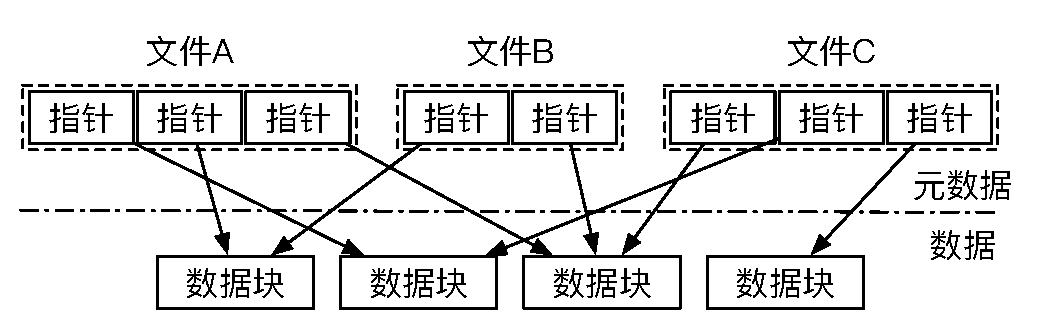
\includegraphics[width=10cm]{DedupSystemStorageMode}
    \caption{数据重删系统的存储模式} 
    \label{fig:数据重删系统的存储模式}
\end{figure}

为了保护数据隐私,加密重复数据删除(encrypted deduplication)增加了一层作用于逻辑数据块的加密操作。如图\ref{fig:加密重复数据删除系统逻辑视图}所示,该加密层基于数据内容来产生加密密钥\citing{bellare2013message}(例如将数据块的哈希值作为密钥\citing{douceur2002reclaiming}),从而将相同的明文数据块加密为相同的密文数据块。系统计算每个密文数据块的哈希值(称为指纹,fingerprint),查询指纹索引(fingerprint index)确定该数据块是否已经存储,最后保存仅具有唯一指纹的密文数据块。需要指出的是,部分加密重复数据删除方案\citing{bellare2013message}采用随机加密算法,但基于明文数据块产生指纹,因此仍然可以通过检查指纹来识别重复数据。

\begin{figure}[!htb]
    \small
    \centering
    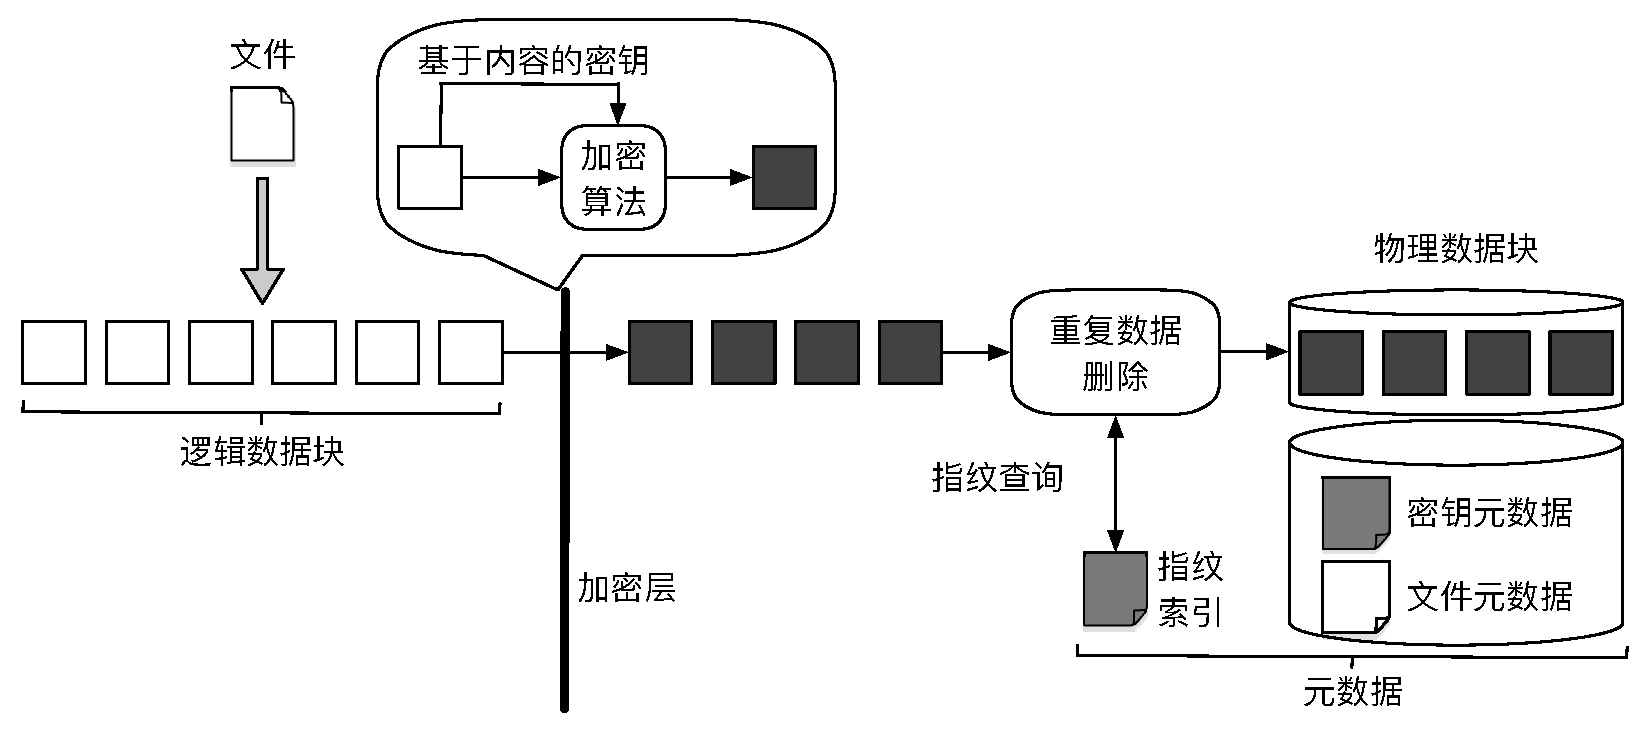
\includegraphics[width=14cm]{EncryptDedupSystemLogic}
    \caption{加密重复数据删除系统逻辑视图}
    \label{fig:加密重复数据删除系统逻辑视图}
\end{figure}

除了指纹索引以外,加密重复数据删除系统须存储额外的元数据(metadata),包括:
\begin{enumerate}
    \item 文件元数据记录了文件内逻辑数据块与相应物理数据块的映射关系,用于重构完整文件。
    \item 密钥元数据记录了文件内逻辑数据块的解密密钥,用于恢复相应的明文内容,由于密钥元数据包含密钥信息,需由文件属主的主密钥(master key)加密后以密文形式存储。
\end{enumerate}

\subsection{问题和动机}

\textbf{密钥生成的安全性和效率平衡问题}

%TODO:数据块信息引用
由于基于数据块内容产生密钥,加密重复数据删除泄漏了数据块的频率信息,即如果一个明文数据块出现了n次,则它对应的密文数据块也将出现n次。另一方面,真实数据集中数据块的出现频率往往呈非均匀分布,调研了FSL和VM备份数据集的数据块频率分布特征,发现三种数据集有超过97\%的数据块的频率低于100次,而至多只有0.04\%的数据块的频率高于10,000次(图\ref{fig:两种真实数据集的数据块频率分布}),这种非均匀的分布特点使攻击者可以利用频率来确定相应数据块。

基于以上原因,认为加密重复数据删除可能受到频率分析\citing{naveed2015inference}的威胁,拟通过本课题,深入研究频率分析攻击对加密重复数据删除安全性的影响,以及提高频率分析攻击效果的方法。

\textbf{重复数据删除中的安全性和效率平衡问题}

从\ S \ ref {sec:introduction}中回想起,现有的加密重复数据删除实现需要昂贵的密码保护。 服务器辅助的MLE必须使用OPRF协议\ cite {naor04}来保护指纹信息免受密钥服务器的侵害,但是OPRF协议涉及昂贵的公钥加密操作(请参见\ S \ ref {subsec:synthetic}中的Exp \#1 )。 同样,当前的PoW实现基于Merkle树协议\ cite {halevi11},该协议对块级PoW执行许多哈希计算。 尽管我们可以通过在每个文件的基础上应用PoW来减轻PoW的计算量(即客户端证明其拥有文件所有权),但是云无法在基于块的重复数据删除下验证块是否属于文件。 现有的提高服务器辅助MLE或PoW性能的解决方案通常会牺牲安全性\ cite {li20b,xu13,pietro12},带宽效率\ cite {harnik10,li15}或存储效率\ cite {zhou15,qin17,li20b}(\ S \ ref {sec:related_work})。


\subsection{研究意义}

本课题研究将填补频率分析攻击研究空白,对理解加密重复数据删除的实际安全性,并降低其在非适合场景下的误用风险具有重要作用。

尽管加密重复数据删除的频率泄漏已是学术界公认的安全问题,但针对性的频率分析攻击研究仍为空白(即利用频率泄漏来获取隐私数据仍是一个开放性问题),致使部分厂商盲目地将加密重复数据删除技术应用于商业产品\citing{MEGA,ElephantDrive}和开源系统\citing{Cryptosphere,Freenet,GNUP2P,Tahoe-LAFS}中。本项目将研究加密重复数据删除技术在频率分析攻击下的实际安全性,以指导其在适合场景下被正确使用。


\section{国内外研究历史与现状}

\subsection{加密重复数据删除}
\label{sec:加密重复数据删除}
在传统对称加密方式下,每个用户具有不同的密钥,不同用户之间的相同明文会被加密为不同密文,难以执行(密文)重复数据删除操作。

消息锁定加密(message-locked encryption,MLE)确立了加密重复数据删除的密码学基础\citing{bellare2013message}:基于数据内容产生密钥(称为 MLE 密钥),从而将相同明文加密为相同密文。最流行的MLE实例是收敛加密(convergent encryption,CE)\citing{douceur2002reclaiming},它使用明文的哈希值作为MLE密钥,并基于密文哈希值计算指纹,以识别重复数据(如图\ref{fig:加密重复数据删除系统逻辑视图})。基于CE的加密重复数据删除方案还包括:

\begin{enumerate}
    \item 哈希收敛加密(hash convergent encryption,HCE)\citing{douceur2002reclaiming}与CE具有相同的MLE密钥产生规则,但基于明文哈希值计算指纹。
    \item 随机收敛加密(random convergent encryption,RCE)\citing{douceur2002reclaiming}使用随机密钥加密以产生非确定的密文,同时也基于明文哈希值来进行重复检查。
    \item 收敛扩散(convergent dispersal,CD)\citing{li2016cdstore}使用明文哈希值作为秘密共享(secret sharing)的输入种子,在兼容重复数据删除的基础上 提高了密文存储的可靠性。
\end{enumerate}

上述MLE实例基于明文产生MLE密钥(CE、HCE和CD)或指纹(HCE和RCE),如果明文是可预测的(即所有可能的明文的数量有限),这些方案易于受到离线暴力破解攻击\citing{bellare2013message,keelveedhi2013dupless}。为了抵御该攻击,DupLESS\citing{keelveedhi2013dupless}基于第三方密钥服务器实现了服务器辅助 MLE(server-aided MLE),确保无法从离线明文派生出相应的MLE密钥。以服务器辅助MLE为基础,现有研究进一步解决了加密重复数据删除的故障容错\citing{li2015cdstore,duan2014distributed}、透明价格模型\citing{armknecht2015transparent}、点对点密钥管理\citing{liu2015secure}、层次密钥管理\citing{zhou2015secdep}等问题。围绕MLE扩展功能的一系列研究包括:兼容加密重复数据删除的数据完整性审计协议\citing{li2016secure};支持动态访问控制的加密重复数据删除系统REED\citing{li2016rekeying,qin2017design}。

无论是MLE还是服务器辅助MLE,均须为相同的明文产生相同的密文(CE、HCE、CD和DupLESS)或指纹(HCE和RCE),泄漏了数据的出现频率。一些理论研究\citing{abadi2013message,stanek2014secure,bellare2015interactive}基于零知识证明、全同态加密、双线性对运算等底层密码技术实现了随机加密,但这些方案存在计算复杂性高、依赖多轮信息交互等问题,难以应用到系统实践中。本文关注可实际应用的加密重复数据删除系统/方案的频率泄漏问题,研究其安全性影响和防御对策。

\subsection{数据所有权证明}
\label{sec:数据所有权证明}

Source-based deduplication is bandwidth-efficient but vulnerable to
side-channel attacks \cite{harnik10} (\S\ref{subsec:encrypted-dedup}). 
Prior studies \cite{harnik10, li15} combine source-based deduplication and
target-based deduplication to defend against side-channel attacks, while
\sysname achieves
significantly more bandwidth savings by purely performing source-based
deduplication (\S\ref{subsec:real-world}) and using PoW to protect against
side-channel attacks.  Also, \sysname is much more efficient than
Merkle-tree-based PoW (\S\ref{subsec:synthetic}).  Some other studies make PoW
efficient by relaxing security (e.g., \cite{pietro12,xu13}), while \sysname
uses client-side SGX to preserve the security of PoW.

\subsection{基于SGX的存储系统}
\label{sec:基于SGX的存储系统}

SGX \cite{sgx} has been widely used for
securing storage systems.  PESOS \cite{krahn18}  enforces the access policies
of object storage with SGX.  OBLIVIATE
\cite{ahmad18} enhances the security of SGX-based file systems against
privileged side-channel attacks. EnclaveDB \cite{priebe18} and ObliDB
\cite{eskandarian19} protect outsourced databases against information leakage
via SGX.  NEXUS \cite{djoko19} enables fine-grained access control with SGX
over untrusted cloud storage.
On the performance side, Harnik {\em et al.} \cite{harnik18} propose
guidelines on mitigating the performance overhead of SGX implementations.
ShieldStore \cite{kim19} implements application-specific
data management to limit the enclave memory usage.  SPEICHER \cite{bailleu19}
is an SGX-based LSM-based key-value store with efficient I/O operations.  

% to address the I/O performance bottleneck
% of enclave.

All the above studies do not consider deduplication. Dang {\em et al.}
\cite{dang17} propose proxy-based protocols for bandwidth-efficient encrypted
deduplication, but the protocols do not address the key generation performance
overhead and have no implementation. SPEED \cite{cui19} leverages deduplication
to make SGX computations efficient, but \sysname improves the performance of
encrypted deduplication with SGX.  SeGShare \cite{fuhry20} maintains a
cloud-side enclave for secure file-based deduplication, while \sysname uses a
client-side enclave to implement an efficient PoW protocol and supports more
fine-grained chunk-based deduplication. 


\section{课题的研究内容、研究目标、以及拟解决的关键问题}
\subsection{研究内容}

% \subsubsection*{加密重复数据删除的频率分析攻击}

% 在传统频率分析模式下,攻击者能够访问明文逻辑数据块集合M和密文逻辑数据块集合$C$($M$和$C$包含重复的明文和密文数据块)。攻击者根据出现频率分别对$M$和$C$中的数据块进行排序,然后将$C$中的密文数据块映射为$M$中与其具有相同排名的明文数据块。但是,传统频率分析在加密重复数据删除中难以形成有效的攻击,主要原因是:$M$和$C$的原始内容可能存在差异(例如$M$和$C$来源于同一个文件系统在不同时间点的备份镜像),将打乱数据块频率排序的对应关系;并且,在频率排序过程中可能存在大量明文和密文数据块具有相同的频率,频率分析难以排序这些数据块来形成正确的对应关系。

% 为了提高传统频率分析的攻击效果,首先研究基于数据特征的新型频率分析攻击技术。然后,分别从抵抗频率排序干扰和降低攻击发生条件两方面改进攻击技术。最后,实现针对真实系统的频率分析攻击原型,并分析该攻击对各类数据安全性的影响。


\subsection{研究目标}

针对以上研究内容,预期实现如下研究目标: 
\begin{enumerate}
    \item 在理论上,设计基于可信计算硬件的密钥生成和数据块所有权证明机制,并在相应安全假设下论证其安全性。
    \item 在技术上,以理论研究为支撑,设计并实现符合安全性假设的低开销的服务器辅助密钥生成和安全且高效的重复数据删除,设并在真实系统中进行理论验证和攻击效果测试。 
\end{enumerate}


\subsection{拟解决的关键问题}

本课题致力于解决传统服务器辅助密钥生成机制和客户端重复数据删除场景下的数据块所有权证明机制的效率问题,难以解决的如下问题:

\begin{enumerate}
    \item How should enclaves be managed?
    \begin{itemize}
        \item Enclave startup incurs high overhead due to remote attestation
        \item Key enclave needs to manage system wide secret information κ
        \item Client machine cannot persistently maintain enclaves
    \end{itemize}
    \item How does key manager prevent online brute force attack?
    \begin{itemize}
        \item Need to enable revocation on clients’ querying key generation oracle
    \end{itemize}
    \item How can key generation performance be further improved?
    \begin{itemize}
        \item Expensive overhead in establishing secure channel (taking ~70\% overallkeygen overhead)
    \end{itemize}
\end{enumerate}


    


    


\section{拟采取的研究方案}
\label{sec:技术路线}



如图\ref{fig:技术路线图}所示,在支撑研究(基于数据块局部性的频率分析攻击方案\citing{li2017information})的基础上,根据相对频率分布特性,设计抗排序干扰的攻击方法;在数据相似性的基础上,设计低依赖条件的攻击方法。最终设计出针对加密重复数据删除方案/系统的新型频率分析攻击方法及对应的原型软件工具。

\begin{figure}[!htb]
    \small
    \centering
    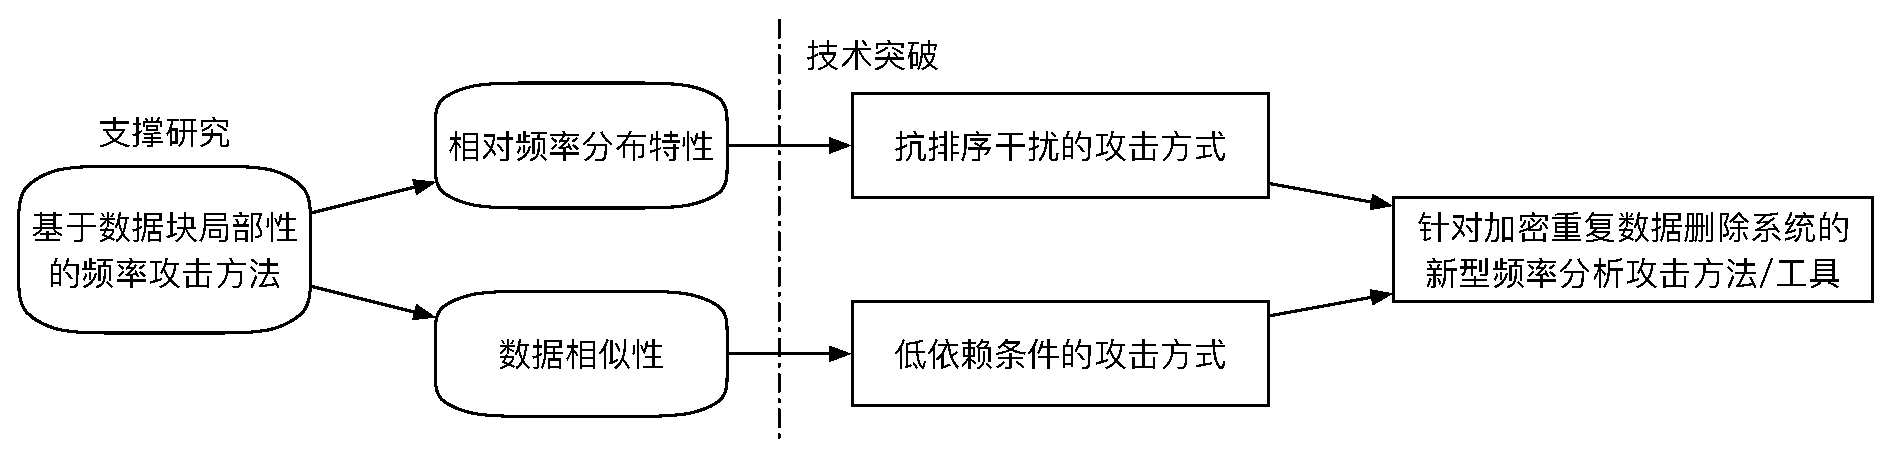
\includegraphics[width=15cm]{TechnicalRoute.eps}
    \caption{技术路线图} 
    \label{fig:技术路线图}
\end{figure}

\subsection{支撑研究}

% 基于数据块局部性的频率分析攻击方案(locality-based attack)\citing{li2017information}作为支撑研究,该方案主要用于破译加密数据备份,即已知的明文数据块集合$M$和目标密文数据块集合$C$源于同一个系统在两个不同时间点的备份镜像。攻击利用了数据块的局部性特征:在不同备份之间,绝大多数数据块保持了相同的局部顺序;例如,每天备份工作项目的进度快照,若一天内的改动较小,则在两次备份之间未被改动的大部分数据块之间的相对顺序保持不变。因此,得出一个关键推论:如果明文数据块M是密文数据块$C$的原始明文,那么M左边和右边相邻的明文数据块有较大可能也是$C$左边和右边相邻密文数据块的原始明文。

% \begin{figure}[!htb]
%     \small
%     \centering
%     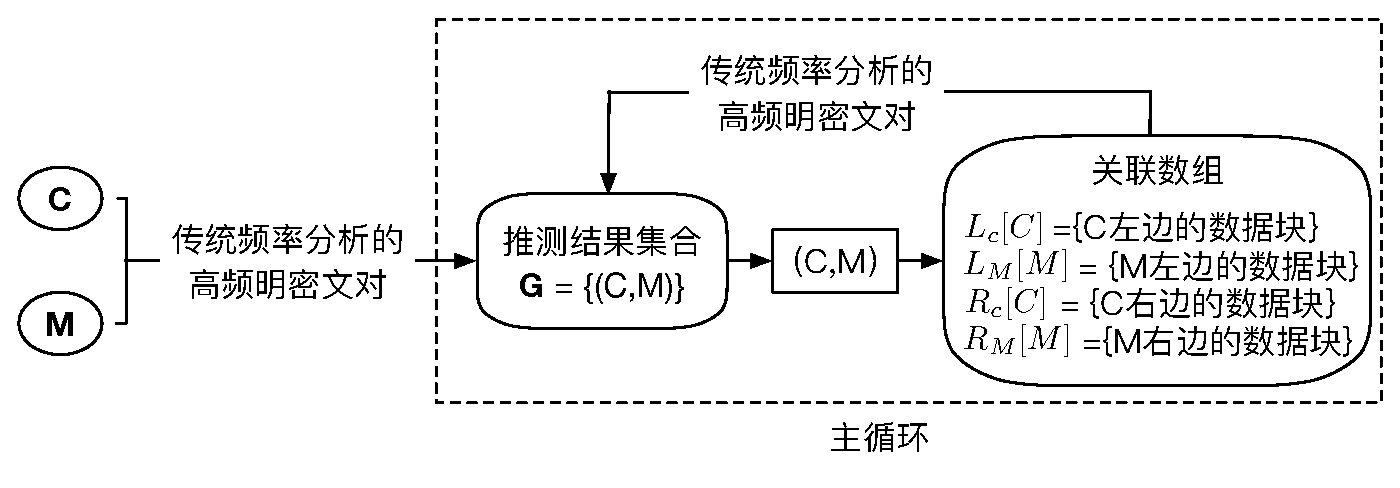
\includegraphics[width=14cm]{BaseFrequencyAttack}
%     \caption{基于数据块局部性的频率分析攻击} 
%     \label{fig:基于数据块局部性的频率分析攻击}
% \end{figure}


% 基于此,攻击流程如图\ref{fig:基于数据块局部性的频率分析攻击}所示:首先,对$C$和$M$应用传统频率分析(\ref{sec:传统频率分析攻击}),将获得的若干组高频明密文对加入推测结果集合 $G$;然后,每次从$G$中选取一组明密文对$(M,C)$,分别对其左右相邻的明文和密文数据块集合$L_M[M]$和$L_C[C]$,以及$R_M[M]$和$R_C[C]$实施频率分析,并将获得的高频明密文对也加入$G$;继续对$G$中的明密文对进行基于相邻数据块的频率分析,直至所有明密文对都被处理。

% 为了验证攻击效果,定义推测率为正确推测出原始明文的(不同)密文数据块个数与$C$中(不同)密文数据块总个数的比率。在基于真实数据集的实验验证中,攻击方案能够达到17.8\%推测率,远远高于传统频率分析方法的0.0001\%推测率。


% \subsection{技术突破}

% \subsubsection{基于分布的频率分析攻击方法}


% \par 基于分布的频率分析攻击利用密文和明文的相对顺序信息来增强频率分析的有效性。该攻击方法建立在数据块局部性\citing{xia2011silo,lillibridge2009sparse,zhu2008avoiding}的基础上。通过以下三个关键特性构造出基于分布的频率分析攻击方法。

% \begin{itemize}
%     \item 数据块局部性指出数据的原始排序可能会在各种备份文件中得以保留,因此可以用于在备份文件中推理出类似的与位置相关的密文-明文对。
%     \item 相邻数据的共现频率的相对频率分布可以通过分析得到。
%     \item 明文及其相应的密文具有相似的相对频率分布的特性。
% \end{itemize}
 
% \subsubsection{基于聚类的频率分析攻击方法}


% 在基于分布的频率分析攻击方法的基础上,通过引入相似性\citing{bhagwat2009extreme}这一属性来消除基于分布的频率分析攻击方法对明文数据的细粒度顺序信息的需求。基于此提出基于聚类的频率分析攻击方法。

\section{可行性分析}

\subsection{研究方法可行}

本课题通过引入加密重复数据删除方案/系统的相关特性来设计新型频率分析攻击方法,针对性提高频率分析攻击方法的有效性。该研究问题具有很高的实际价值且在面向加密重复数据删除的攻击中,已有工作提出了基于数据块局部性(chunk locality)\citing{zhu2008avoiding,lillibridge2009sparse,xia2011silo}的频率分析攻击\citing{li2017information},在此基础上改进攻击方案以提高频率分析攻击实际效果具有明确的可行性。

\subsection{研究条件可行}

前期基于数据块局部性的频率分析攻击方案给出了本课题研究两种新型频率分析攻击方法的基本理论和工具基础。在原有方案上改进即可用于本课题研究。研究者在本科阶段深入钻研了CDStore、REED、SDFS等加密重复数据删除系统,以及前期基于数据块局部性的频率分析攻击方案的理论和工具实现。这些经验可以帮助设计新型频率分析方法以及其在真实系统中的实践。

\section{本研究特色与创新之处}

本研究的特色与创新之处有以下几点:

% \begin{enumerate}
%     \item 研究针对加密重复数据删除提出了两种新型的频率分析攻击方法。除了利用由于加密重复数据删除具有确定性导致的频率泄漏之外,两种攻击都利用重复数据删除工作负载的特性来增加频率分析攻击的有效性。
%     \item 本文研究使用多个真实数据集(包括长期备份\citing{sun2016long,FSL14},Windows文件系统快照\citing{meyer2012study}和VM磁盘映像\citing{li2016cdstore,qin2017design})以及开源重复数据删除系统SDFS\citing{SDFS}、Destor\citing{Destor},评估两种新型频率分析攻击方法和基本频率分析攻击方法的实际效果。通过评估频率攻击方法的攻击结果,进一步分析本频率分析攻击方法对实际加密重复数据删除带来的安全性影响。
%     \item 本研究讨论了减少加密重复数据删除中信息泄漏的可能方案。
% \end{enumerate}

We propose \sysname, a high-performance SGX-based encrypted deduplication
system. \sysname builds on server-aided MLE as in DupLESS \cite{bellare13b},
but executes efficient OPRF-less MLE key generation and PoW inside enclaves.
In particular, it comprises three major building blocks:
%
\begin{itemize}[leftmargin=*] 
\item 
{\em Secure and efficient enclave management}: It protects against the
compromise of the key server and allows a client to quickly bootstrap an
enclave after a restart.
\item 
{\em Renewable blinded key management}: It generates a blinded key for
protecting the communication between the enclave inside the key server and
each of the clients based on key regression \cite{fu06}, such that the blinded
key is renewable for dynamic client authentication. 
\item 
{\em SGX-based speculative encryption}:  It offloads the online
encryption/decryption overhead of an enclave via speculative encryption
\cite{eduardo19}. 
\end{itemize}
\chapter{相关基础研究}
\label{chapter:background}

本章将介绍普通和加密后重复数据删除、可信执行环境(TEE)等本文利用的基础知识,以及加密后重复数据删除系统中存在的性能瓶颈和安全性隐患。

\section{重复数据删除}
\label{sec:background-deduplication}

本文专注于基于数据块的重复数据删除,它以称为数据块的小型数据单元为粒度运行。基于数据块的重复数据删除比基于文件的重复数据删除更精细,因此通常具有更高的存储效率(节省更多的存储空间)。

基于数据块的重复数据删除有以下两种基本的数据块分块方法:

\begin{itemize}[leftmargin=*]
    \item \textbf{固定大小的数据分块(Fixed-size chunking)},通常将文件划分为固定长度的数据块,具有简单快速的特点,但文件中小范围修改(例如:增加1字节内容或删除1字节内容)将从修改位置开始影响后续所有数据块的内容,不利于重复数据删除。
    \item \textbf{可变大小的数据分块(Variable-size chunking)},也称为内容定义的数据块分块(Content-defined chunking)。通常采用内容相关的方式指定数据块的边界(例如,通过Rabin指纹\cite{rabin1981fingerprinting}在特定内容模式出现时进行分块)。因此,在文件发生小范围修改时,产生的大多数数据块仍可保持不变,使得重复数据删除系统存储效率得到保障。
\end{itemize}

在多数备份系统工作负载\cite{zhu2008avoiding,lillibridge2009sparse}下,可变大小的数据分块方案通常可以获得更优的存储效率,但在某些特定工作负载(例如,VM备份数据集\cite{jin2009effectiveness})下,固定大小的数据分块方案却更加有效。本文的工作可兼容固定大小和可变大小的数据分块方法产生的数据块。

\begin{figure}[!htb]
    \small
    \centering
    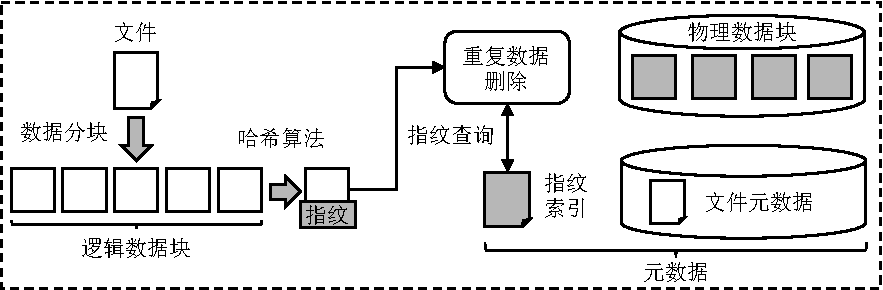
\includegraphics[width=\textwidth]{chunk-based-dedup-arch.pdf}
    \caption{基于数据块的重复数据删除的工作流程概览}
    \label{fig:chunk-based-dedup-flow}
\end{figure}

图\ref{fig:chunk-based-dedup-flow}总结了基于数据块的重复数据删除工作流程。具体地,重复数据删除系统首先通过数据分块过程将客户端的文件(例如,备份文件)分割为逻辑数据块,根据每一个逻辑数据块的内容,使用哈希算法计算得到其对应的唯一标签(又称为指纹)。如果两个数据块具有相同的指纹,则认为两个数据块内容相同(不同逻辑数据块计算得到相同指纹的概率可忽略不计\cite{black2006compare});若两个逻辑数据块指纹不一致,则认为两逻辑数据块不同。重复数据删除系统仅存储相同逻辑数据块的唯一副本(称为物理数据块),并且每个相同的逻辑数据块仅通过一个空间开销较小的索引指向相同的物理数据块。此外,基于数据块的重复数据删除系统记录文件所拥有的所有逻辑数据块的信息作为该文件的元数据,用于文件读取、删除等操作。

重复数据删除技术根据重复数据删除操作发生的位置可分为源端重复数据删除及目标端重复数据删除\cite{IDC2010Data}:

\begin{itemize}[leftmargin=*]
    \item \textbf{源端重复数据删除(Source-based Deduplication)}由客户端计算目标数据块的哈希值,并由服务端检查该哈希值是否存在于索引表中。如果哈希值存在(即服务端已有目标数据块的副本),则通知客户端无需传输目标数据块。
    \item \textbf{目标端重复数据删除(Target-based Deduplication)}强制客户端传输所有密文数据块,并在服务端对所有收到的密文数据块进行重复数据删除。
\end{itemize}

源端重复数据删除技术可有效节省网络流量资源,可显著降低云服务商提供存储服务的成本,但泄露了“其他客户端是否已经存储相应密文数据块”的侧信道信息(参见\S\ref{subsubsec:intro-problem-security});目标端重复数据删除具有更高的隐私保护能力,但产生大量网络资源浪费,并显著增加了服务端计算开销。本文关注网络资源开销较小的源端重复数据删除技术,并通过TEE技术解决其存在的性能和安全性问题。

\section{安全重复数据删除}
\label{sec:background-enc-deduplication}

加密后重复数据删除解决了外包环境(例如,云存储)中的数据块机密性保障问题,同时保持了重复数据删除的有效性。出于安全因素考虑,用户希望将自己的数据加密后再进行外包存储,以确保个人数据隐私性。传统对称加密算法算法为每个客户端或每个逻辑数据块分配独立的加密密钥,使得来自不同(或相同)客户端的相同的逻辑数据块被加密为不同的密文数据块,服务器无法感知这些密文数据块所对应的明文数据块内容是否一致,使得针对外包数据的重复数据删除完全失效。

\begin{figure}[!htb]
    \small
    \centering
    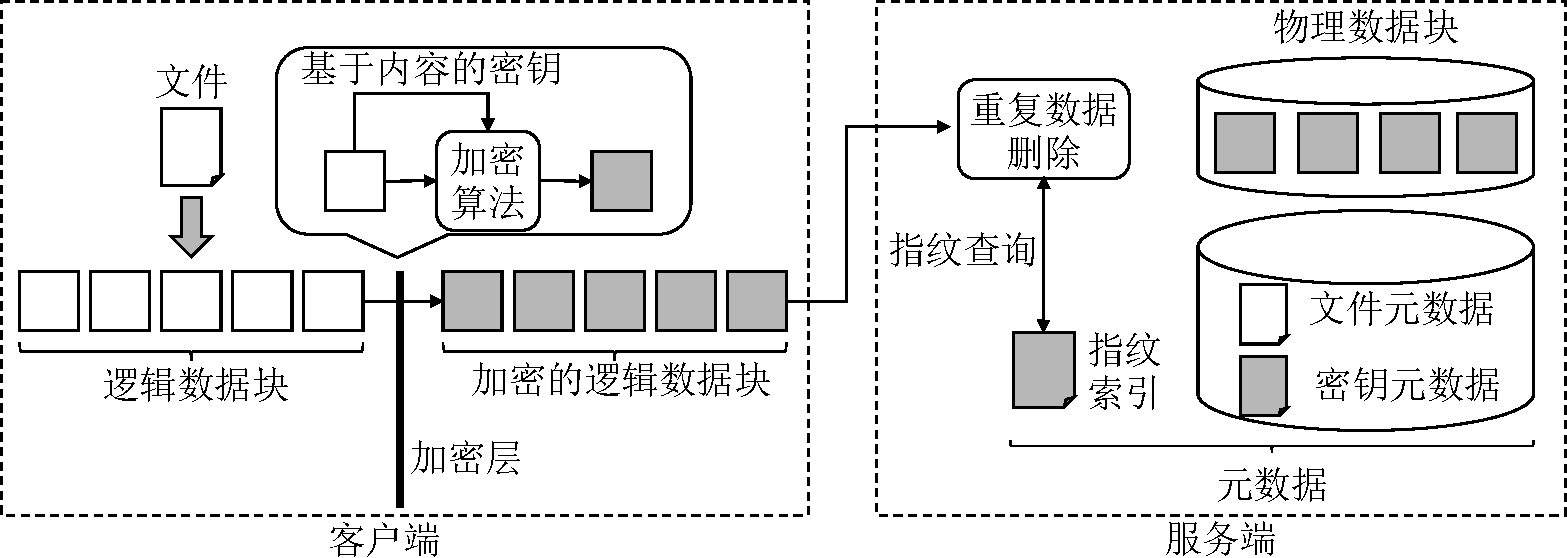
\includegraphics[width=\textwidth]{chunk-based-enc-dedup-arch.pdf}
    \caption{基于数据块的加密后重复数据删除的工作流程概览}
    \label{fig:chunk-based-enc-dedup-flow}
\end{figure}

如图~\ref{fig:chunk-based-enc-dedup-flow}所示,基于内容的密钥生成方法给加密后重复数据删除提供了新的处理思路。最基本的基于内容的密钥生成方法的实例化是基于明文数据的内容(例如,基于重复数据删除中的逻辑数据块)导出其对称加密密钥,并使用该密钥加密明文数据以形成对应的密文数据(例如,加密的逻辑数据块)。因此,使用基于内容的密钥生成方法为任意逻辑数据块产生对称加密密钥可以确保将相同的明文数据块加密为相同的密文数据块。最后,存储系统从每个密文数据块中导出其对应的指纹并执行重复数据删除。相较于普通重复数据删除,加密后重复数据删除需额外保存用户文件所包含数据块的密钥元数据,并由各个客户端进行加密以防止服务端取得相应数据块的明文内容。

\subsection{数据块加密技术}
\label{subsec:background-encrypted-deduplication-key}

\textit{消息锁加密(Message-Locked Encryption, MLE)}\cite{bellare2013MLE}将基于内容的密钥生成方案等加密原语形式化用于加密后重复数据删除。它指出了如何从明文数据块的内容导出相应的对称加密密钥(称为 \textit{消息锁加密密钥(MLE密钥)})。以最广泛使用的消息锁加密技术:收敛加密(Convergent Encryption, CE)\cite{douceur2002reclaiming}为例,CE使用明文数据块的安全哈希作为MLE密钥,使得相同的明文数据块可被加密为相同的密文数据块,从而令重复数据删除技术在密文数据块之上仍然可行。除此之外,基于CE的消息锁加密方案还包括:

\begin{enumerate}[leftmargin=*]
    \item \textbf{哈希收敛加密(Hash Convergent Encryption, HCE)}\cite{douceur2002reclaiming}与CE具有相同的MLE密钥产生规则,但基于明文哈希值计算指纹用于重复数据删除(CE使用密文指纹进行重复数据删除)。
    \item \textbf{随机收敛加密(Random Convergent Encryption, RCE)}\cite{douceur2002reclaiming}使用随机密钥加密明文以产生非确定的密文,但基于明文的哈希值进行重复数据删除检查。
    \item \textbf{收敛扩散(Convergent Dispersa, CD)}\cite{li2016cdstore}使用明文哈希值作为秘密共享(Secret Sharing)的输入种子,并对产生的多个秘密共享分别计算哈希并进行重复数据删除,在兼容重复数据删除的基础上提高了密文存储的可靠性。
\end{enumerate}

然而,CE容易受到\textbf{离线暴力破解攻击}的威胁。这是由于CE的MLE密钥(即明文数据块的哈希)可以自由产生。具体来说,攻击者通过枚举所有可能的明文数据块的MLE密钥来从目标密文数据块(其加密密钥未知)推断输入的明文数据块,以检查是存在某个明文数据块被加密到目标密文数据块。

服务器辅助消息锁加密(Server-aided MLE)\cite{bellare2013DupLESS}是最先进的加密原语,可增强加密后重复数据删除对离线暴力攻击的安全性。它为消息锁加密中的MLE密钥生成步骤部署了一个专用的\textbf{密钥服务器(key server)}。为了加密明文数据块,客户端首先将明文数据块的指纹发送到密钥服务器,密钥服务器通过指纹和密钥服务器维护的\textbf{全局秘密(global secret)}返回MLE密钥。如果全局秘密是安全的,则攻击者无法发起离线暴力攻击;如果全局秘密被泄露,则其安全性会降低到原始消息锁加密的安全性。服务器辅助消息锁加密建立在如下两种安全机制之上:

\begin{itemize}[leftmargin=*]
    \item \textbf{遗忘伪随机函数(oblivious pseudorandom function, OPRF)}\cite{naor2004Number}是一种安全计算协议,协议包含服务端和客户端,服务端持有密钥$k$,客户端持有输入$x$,双方通过交互来联合计算函数$f_k(x)$,最终由客户端得到函数值。OPRF的计算过程以盲化方式进行,即在计算过程中服务端无法获取关于$x$的任何有价值信息,同时客户端无法获取关于$k$的任何有价值信息。
    \item \textbf{速率限制(Rate-limiting)}\cite{bellare2013DupLESS}阻止特定操作频率超出某些限制。在大型系统中,速率限制通常用于保护底层服务和资源。
\end{itemize}

基于遗忘为随机函数,密钥服务器可依据客户端发送明文数据块的“盲化指纹”,进而基于盲指纹和全局秘密产生对应数据块的“盲化密钥”,阻止了密钥服务器了解明文数据块信息;并使得客户端可在不了解密钥服务器所拥有的全局秘密的条件下获得目标明文数据块的MLE密钥。对来自客户端的密钥生成请求进行速率限制,进一步防止恶意客户端向密钥服务器发出海量密钥生成请求以获得目标MLE密钥,限制了攻击者暴力破解攻击的速度。

\subsection{数据所有权证明技术}
\label{subsec:background-encrypted-deduplication-pow}

为了节省宝贵的网络带宽资源,现有加密后重复数据删除系统普遍采用源端重复数据删除,以便在客户端删除重复数据块,而无需上传到服务端(\S\ref{sec:background-deduplication})。但是,源端重复数据删除导致“目标数据块是否已在服务端存储”的侧信道信息,使得某些客户端存在恶意时,源端重复数据删除很容易受到侧信道攻击(\textit{Side-channel Attack})\cite{harnik2010side,halevi11}的影响。

一种典型的侧信道攻击被称为\textbf{伪造所有权攻击}:恶意客户端未授权访问其他客户端存储的数据块\cite{harnik2010side,mulazzani11}。具体来说,由于服务端仅能基于收到的数据块哈希值判断客户端是否拥有对应的数据块,攻击者可使用任意目标密文数据块的指纹来说服服务端其是该目标数据块的所有者,进而获得该数据块的完全访问权限(\S\ref{subsec:intro-background});另一种侧信道攻击被称为\textbf{推测内容攻击}:恶意客户端将目标密文数据块指纹发送到服务端以检查该数据块是否存在(例如,目标密文数据块对应于某个可能的密码\cite{harnik2010side}),以此识别来自其他客户端的敏感信息(\S\ref{subsubsec:intro-problem-security})。

现有防御机制尚无法在执行源端重复数据删除且不大量增加额外网络带宽资源开销的前提是防御推测内容攻击。而为了防止伪造所有权攻击,源端加密后重复数据删除增加了所有权证明(proof-of-ownership, PoW)机制\cite{halevi11},要求客户端额外向服务端提交目标密文数据块的所有权证明(proof),且仅在所有权证明成功的条件下进行重复数据删除。所有权证明机制可使得服务端只针对客户端真实拥有(即具有完整访问权限)的密文数据块执行重复数据删除,避免了攻击者非法访问其他客户端已在云服务端存储的内容。现有基于默克尔树(Merkel Tree)的所有权证明机制(称为POW-MT)\cite{xu2013weak}使用纠删码对数据块进行编码,随后在纠删码编码结果的基础上建立默克尔树用于所有权证明。而另一种基于通用哈希函数(Universal Hash)的所有权证明机制(称为POW-UH)\cite{halevi2011proofs} 相较于基于默克尔树的所有权证明机制拥有更高的效率,但降低了安全性假设。

本文关注网络和服务端计算资源开销较小的源端重复数据删除技术,并通过TEE技术解决其存在的密钥生成和所有权证明效率问题,以及易受到推测内容攻击的安全性问题。

\section{可信执行环境(TEE)}
\label{sec:background-tee}

TEE全名为可信执行环境(Trusted Execution Environment)是计算平台上由软件协同硬件方法构建的一个安全区域,可以确保在安全区域内加载的程序和数据在完整性和机密性方面得到必要保护。其目标是确保目标程序按照预期执行,保证程序初始状态和运行时状态的机密性、完整性。针对TEE的相关概念及规范定义,各个软件、硬件厂商结合自己的基础架构形态产生的具体实现各不相同。虽然在技术实现上存在显著差异,但TEE的技术共同点可总结为如下三点:

\begin{itemize}[leftmargin=*]
    \item \textbf{隔离性}:
          TEE通过隔离的程序执行环境,提供一个可信的执行空间,为其中运行的程序和存储的数据提供了机密性和完整性保护。X86架构的隔离机制从Intel 80286处理器开始,Intel提出了CPU的两种运行模式,并且逐步衍生出后来的不同的特权界别,再后来提出了安全区域范围更小的SGX机制实现可信执行环境(TEE);同样的,ARM架构通过TrustZone技术实现了相关软硬件的隔离性,实现了安全世界(Secure World)与非安全世界(Normal World)的隔离。
    \item \textbf{软硬协同性}:
          虽然标准定义可以通过单独软件方式或单独硬件方式实现TEE,但实际应用场景下,行业内更多选择通过软硬件结合的方式进行TEE的设计。
    \item \textbf{富表达性}:
          与传统安全新芯片或纯软件的密码学营私保护方案相比,TEE支持的上层业务表达性更强,软件开发者仅需要根据业务逻辑划分业务层面的隐私和非隐私区域,而不会对定义隐私区域内的算法逻辑的语言等有可计算性方面的限制(图灵完备的)。同时,由于TEE为程序提供了可信的执行环境,安全区内的数据无需进行密态运算,使得TEE应用可以支持更多的算计及复杂的算法。
\end{itemize}

\subsection{Intel SGX}
\label{subsec:background-tee-sgx}

\begin{figure}[!htb]
    \small
    \centering
    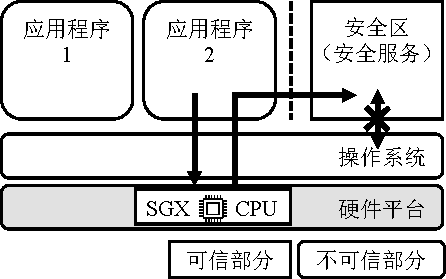
\includegraphics[width=0.6\textwidth]{sgx-example.pdf}
    \caption{Intel SGX框架}
    \label{fig:sgx-arch}
\end{figure}

Intel Software Guard Extensions (Intel SGX)\cite{sgx,sgx2},是一组内置于现代Intel CPU中用于增强应用程序代码和数据安全性的扩展指令。开发者可利用SGX技术将应用程序的安全操作封装在称为“安全区(Enclave)”的硬件保护环境中,保障用户关键代码和数据的机密性和完整性。Intel SGX最关键的优势在于将应用程序以外的软件栈如操作系统(OS)和基本输入输出系统(BIOS)都排除在了可信计算基(Trusted Computing Base, TCB)之外,一旦程序和数据在安全区之中,即便是操作系统和也无法影响安全区内的代码和数据,安全区的安全边界只包含CPU和它本身(如图\ref{fig:sgx-arch}所示)。Intel SGX具有隔离、证明和密封三项主要安全功能。

\textbf{隔离(Isolation)}:安全区代码和数据被放置在被称为\textit{enclave page cache (EPC)}的硬件内存保护区域中,该内存区域使用内存加密引擎(MEE)进行加密,以防止泄露任何内存数据到本安全区之外。EPC以大小为4\,KiB的页面为基本单位管理安全区内存,任意安全区内应用程序最多可占用96\,MiB内存空间\cite{harnik2018SGX}。当安全区内存使用超过上限时,须将未使用的内存页面加密并逐出到未受保护的主存,并在将逐出的页面加载回安全区内存时解密并验证完整性,导致巨大的分页开销\cite{arnautov2016SCONE,dinhngoc2019Everything}。

此外,SGX为安全区和未受保护的内存之间的交互提供了两个接口,应用程序可以通过安全区内部调用(ECalls)进入安全区以执行安全区内部函数,并且在ECall中,程序可通过安全区外部调用(OCalls)暂时退出安全区并调用不受保护的内存中的不受信任的函数。但安全区内部调用和外部调用会产生大量的CPU上下文切换开销\cite{harnik2018SGX},严重影响SGX应用程序性能。

\textbf{认证(Attestation)}:SGX安全区支持本地认证(Local Attestation)和远程认证(Remote Attestation),以确保安全区内运行的程序未被修改。特别的,在远程认证过程(参见\cite{SGX-RA}提供的端到端远程认证示例)中,远程实体(例如,服务端)需要联系Intel运营的证明服务来检查目标安全区提供的安全区相关信息的完整性和正确性。随后,远程实体通过将其收到的安全区信息与目标安全区中预期的可信信息进行比较来验证目标安全区是否未被修改。然而,由于远程认证需要Intel服务器的支持,远程认证过程通常导致较高且不可控的时间开销。

\textbf{密封(Sealing)}: SGX安全区通过密封在安全区内容需要在安全区外持久化存储时进行保护。它使用目标安全区专用的密封密钥(Sealing key)在数据被移出安全区之前进行加密。密封密钥可以从安全区测量哈希(Measurement hash,即安全区内容的SHA-256哈希)或安全区的创建者提供的签名身份派生。基于前者产生的密封密钥仅有目标安全区本身可以导出,而基于后者产生的密封密钥可有同一开发者创建的各个不同的安全区导出。因此,仅有相应的安全区才能获得正确的密封密钥并解密密封数据。

\subsection{ARM TrustZone}
\label{subsec:background-tee-tz}

ARM TrustZone\cite{trustzone}是ARM公司为Cortex-A微架构\cite{cortex-a}设计的一种TEE解决方案,其目的是为其产品构建一个安全框架来抵御各种可能的攻击,它通过对原有硬件架构进行修改,在处理器层次引入了两个不同权限的保护域:安全世界(Secure World)和非安全世界(Normal World),并防止运行于非安全世界的软件直接访问安全世界资源。

如图~\ref{fig:ARM-TZ-base}(a)所示,ARM引入了一种称为监视模式的处理器模式,该模式负责在世界过渡时保留处理器状态,两个世界可以通过称为安全监视器调用(Secure Monitor Call, SMC)的特权指令进入监视模式并实现彼此切换。

\begin{figure}[!htb]
    \small
    \centering
    \begin{tabular}{@{}c@{}c@{}c}
        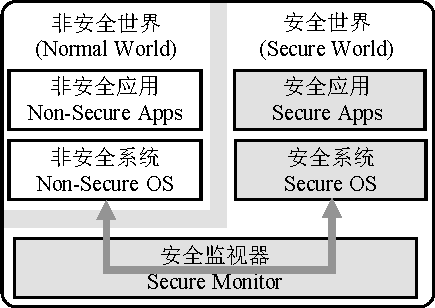
\includegraphics[width=0.49\textwidth]{ARM-TZ-A.pdf} &
        \hspace{5pt}
        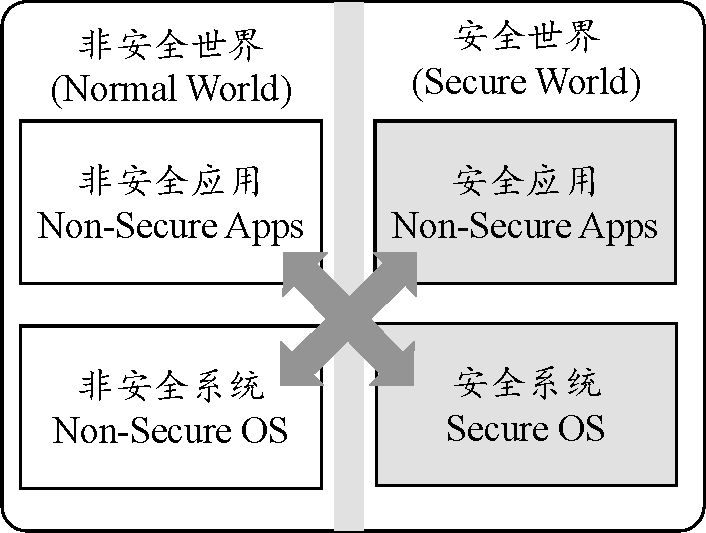
\includegraphics[width=0.49\textwidth]{ARM-TZ-M.pdf}   \\
        \mbox{\small (a) Cortex-A微架构中的TrustZone}        &
        \mbox{\small (b) Cortex-M微架构中的TrustZone}          \\
    \end{tabular}
    \caption{ARM TrustZone技术}
    \label{fig:ARM-TZ-base}
\end{figure}

除了Cortex-A微架构外,ARM发布的新一代Cortex-M微架构\cite{cortex-m}同样为TrustZone提供了硬件支持。与Cortex-A相同的是,Cortex-M依旧将处理器运行状态划分为安全世界和非安全世界,并阻止运行于非安全世界的软件直接访问安全资源。不同的是,Cortex-M针对更快的上下文切换和低功耗应用进行了优化。具体来说,Cortex-M中世界之间的划分是基于内存映射的,并且转换是在异常处理代码中自动发生的(如图~\ref{fig:ARM-TZ-base}(b)所示)。这意味着,当从安全内存运行代码时,处理器处于安全世界,而当从非安全内存运行代码时,处理器处于非安全世界。Cortex-M中的TrustZone技术排除了监视模式,也不需要任何安全的监视软件,这大大减少了安全世界与非安全世界的切换延迟,使得世界之间的转换为更高效。

各芯片产商根据ARM公司对于TrustZone的硬件设计在各自具体的芯片上进行设计和实现,基于TrustZone技术,可以搭建一个可信执行环境(TEE),并在TEE内运行基于TrustZone的操作系统,如高通的QSEE、开源的OP-TEE等。

\section{本章小结}

本章介绍了普通与加密重复数据删除,现有加密重复数据删除中数据块加密技术和数据所有权证明技术导致的性能问题,以及可信执行环境的相关内容。

\chapter{威胁模型}
\label{sec:ThreatModel}
本章为针对加密重复数据删除的频率分析攻击制定了威胁模型。

\section{威胁模型定义}
\label{sec:ThreatModel-Definitions}

本文分别使用$M$和$C$来表示明文数据块(即加密前的逻辑数据块)及其对应的密文数据块(即加密后的逻辑数据块);$|M|$和$|C|$来表示明文数据块(即加密前的逻辑数据块)的大小及其对应的密文数据块(即加密后的逻辑数据块)的大小。

首先将普通文件建模为由$n$个逻辑明文数据块构成的有序列表(即重复数据删除之前的逻辑块),该列表记为$\mathbf{M} = \langle \hat{M}^{(1)}, \hat{M}^{(2)}, \ldots, \hat{M}^{(n)}\rangle$。 每个逻辑明文数据块$\hat{M}^{(i)}$(其中$1\le i\le n$)通过MLE加密得到相应的密文数据块$\hat{C}^{(i)}$。由$\mathbf{M}$的所有加密结果形成由$n$个逻辑密文数据块组成的有序列表记为$\mathbf{C} = \langle \hat{C}^{(1)}, \hat{C}^{(2)}, \ldots, \hat{C}^{(n)} \rangle$。在$\mathbf{C}$中的逻辑密文数据块也会被排序以反映加密重复数据删除存储系统中重复数据删除处理过程的顺序。

相同的逻辑明文和密文可能分别出现在$\mathbf{M}$和$\mathbf{C}$中的不同位置。 本文将一个唯一的明文数据块表示为$M$(通过其指纹的唯一性确定),通过MLE加密得到相应的唯一密文数据块$C$。每个$M$对应于$\hat{M}^{(i)}$的一个或多个相同副本,同理,每个$C$对应于$\hat{C}^{(i)}$的一个或多个相同副本。


\section{对手的目标和相关假设}
\label{sec:ThreatModel-Assumptions}

本文考虑存在一个对手,它准备以以下两个明确的目标为基准推理一组密文数据块-明文数据块对(用\{$(C, M)$\}表示)。


\begin{itemize}
    \item \textbf{推理率高:} 
    
    在所有的正确密文数据块-明文数据块对中,推理出大部分正确的密文数据块-明文数据块对(即统计学上的高召回率或低阴性率)。

    \item \textbf{推理精度高:} 
    
    在所有推理得到的密文数据块-明文数据块对中大部分的密文数据块-明文数据块对的配对是正确的(即统计术语中的高精度或低误报率)。
\end{itemize}
  
  
本文假设该对手是诚实但好奇的,它可以被动地监视密文数据块流$\mathbf{C}$被写入存储系统中的过程,并利用来自$\mathbf{C}$的不同类型的泄漏信息(参见章节:\ref{sec:ThreatModel-Leakage})。鉴于可用的泄漏信息种类,对手仅可通过唯密文攻击的方法推理$\mathbf{C}$中每个密文数据块对应的原始明文数据块。当然,对手也有可能知道有限的密文数据块-明文数据块对的集合来发起已知明文攻击,这种情况进一步加深了攻击的严重性\citing{li2017information}。但在本文中不会考虑前述的已知明文攻击方式。因此,本文将$\mathbf{C}$视为对手所能观察到的的视图,并为该视图的不同属性建模。

本文假设对手无法访问任何包含有关如何操作和存储数据块的信息的元数据(由于不对元数据应用重复数据删除,因此可以通过传统的对称加密来保护这些元数据,这种操作可使得对手无法获知该类型的信息)。此外,本文假设对手没有主动对重复数据删除系统进行攻击的能力,因为这种问题可以通过现有方法予以阻止。例如是恶意客户端可以在客户端重复数据删除中声明对未授权文件拥有所有权\citing{harnik2010side,halevi2011proofs,mulazzani2011dark}; 该问题可以通过所有权证明\citing{halevi2011proofs,xu2013weak,di2012boosting}或服务器端重复数据删除\citing{harnik2010side,li2015cdstore}予以解决。另一个例子是恶意存储系统可以修其改存储的数据;该问题可以通过远程完整性检查来进行检测和解决\citing{juels2007pors,ateniese2007provable}。

\section{三种信息的泄漏}
\label{sec:ThreatModel-Leakage}

本文在加密重复数据删除存储中考虑三种类型的泄漏方式,这些泄漏使得对手能够基于它们推理信息:

\begin{itemize}
    \item \textbf{频率:}  

    由于加密重复数据删除的加密过程的确定性,重复数据删除前$\mathbf{C}$中每个密文数据块的频率(即重复副本数量)可以映射得到$\mathbf{M}$中相应明文数据块的频率。

    \item \textbf{顺序:} 
 
    某些加密重复数据删除存储系统\citing{xia2011silo,lillibridge2009sparse,zhu2008avoiding}为了更高的运行性能,在存储密文数据块是保持了其对应的明文数据块的原始顺序。因此,$\mathbf{C}$中的密文的顺序可以映射到$\mathbf{M}$中的明文的顺序。

    \item \textbf{大小:} 

    可变大小的数据块分块方法(参见章节:\ref{sec:background})产生会产生各种不同大小的明文数据块,如果在对明文数据块进行加密前没有进行数据填充(为了避免增大存储开销\citing{ritzdorf2016information,douceur2002reclaiming,wilcox2008tahoe,keelveedhi2013dupless}),则产生的密文数据块大小与其对应的原始明文数据块大小一致($\mathbf{C}$中的密文大小可以映射到$\mathbf{M}$中相应明文的大小)且密文数据块集合中的密文数据块也具有众多不同的大小。当然,该泄漏可以通过使用块密码算法使得明密文数据块大小不一致来避免。
\end{itemize}

除上述三种泄漏以外,对手还可以获得一些辅助信息,这些信息提供了与$\mathbf{M}$相关的数据特征的基本情况(任何推理攻击都必须提供辅助信息\citing{kumar2007anonymizing,li2017information,grubbs2016breaking,zhang2016all,kellaris2016generic,ritzdorf2016information,naveed2015inference,cash2015leakage,islam2012access})。在这项工作中,将辅助信息视为先前已知的明文数据块(例如,通过旧用户备份或VM磁盘映像得到)构成的有序列表,由$\mathbf{A}$表示。显然,攻击有效性与严重性取决于$\mathbf{A}$(即先前已知的明文数据块)和$\mathbf{M}$(即要推理的明文数据块)之间的相关性。本文的重点不是解决对手如何获取辅助信息的问题。例如,可能是由于粗心的数据发布\citing{careless-release}、被的盗存储设备\citing{stolen-device}和云存储泄漏\citing{cloud-leakage}。相反,根据这些信息,本文研究了可以获得的的辅助信息如何与各种泄漏渠道相结合,给加密重复数据删除带来信息泄漏。

本文将频率分析\citing{al1992origins}作为攻击方法。经典频率分析对$\mathbf{C}$中的唯一密文数据块和$\mathbf{A}$中的唯一明文数据块按频率(即对应于每个唯一密文数据块或唯一明文数据块的相同副本的数量)进行排序。然后,简单的将$\mathbf{C}$中的每个唯一密文数据块与$\mathbf{A}$中具有相同频率等级的唯一明文数据块相关联。基本的频率分析攻击实际效果非常糟糕,在接下来的章节中,本文针对加密重复数据删除设计了较为复杂同时效性极高的频率分析攻击。

\section{本章小结}

本章介绍了针对重复数据删除的威胁模型的定义、本课题研究中将要用到的各种信息来源,以及本文攻击方案的假设的相关说明。






\chapter{基于分布的频率分析攻击方法}
\label{sec:DistributionAttack}

基于分布的攻击利用$\mathbf{C}$和$\mathbf{A}$的数据块的逻辑顺序信息来增强频率分析的有效性。它通过比较$\mathbf{C}$和$\mathbf{A}$的相对频率分布,以减少误报结果。本文还展示了如何利用数据块的大小信息来进一步提高推理精度。

\section{背景知识:基于数据块局部性的频率分析的攻击}

\label{sec:DistributionAttack-prior-attack}

基于分布的频率分析攻击建立在已有的基于数据块局部性的频率分析攻击\citing{li2017information}的基础上,它展示了频率分析如何导致备份工作负载中的信息发生泄漏。基于数据块局部性的频率分析攻击针对每日或每周为主要数据的完整副本(例如,应用程序状态,文件系统快照和VM磁盘映像)创建的完全备份(简称为备份)。它旨在推理不同版本备份间的密文数据块-明文数据块对。它通过假定辅助信息$\mathbf{A}$来自一些较旧的备份,来推理最新备份的明文数据块(即$\mathbf{M}$)。

基于数据块局部性的频率分析攻击利用了数据块局部性这一属性\citing{xia2011silo,zhu2008avoiding,lillibridge2009sparse},这是实际备份工作负载中的常见现象。 具体而言,局部性是指在重复数据删除之前,相邻的数据块在不同版本的备份中往往以相同的逻辑顺序存在。 主要原因是每个备份的更新通常聚集在一些小范围内的数据块中,而剩余的大范围内的数据块在不同版本的备份中保持不变(保持相同的顺序)。

根据局部性原理,基于数据块局部性的频率分析攻击利用逻辑顺序信息来发现密文数据块和明文数据块的邻近信息。具体来说,对于给定的唯一密文数据块$C$,对手首先标识所有相同副本的集合$\{\hat{C}^{(i)}\}$。对于每个$\hat{C}^{(i)}$,它会考虑$\hat{C}^{(i)}$的左右邻居,即$\hat{C}^{(i-1)}$和$\hat{C}^{(i+1)}$。它将左右邻居的集合分别提取到关联数组$\mathbf{L_C}$和$\mathbf{R_C}$中。关联数组分别存储每个唯一密文$C$的映射及其与左右邻居的共现频率。同时,对手还会根据$\mathbf{A}$的逻辑顺序信息构造关联数组$\mathbf{L_A}$和$\mathbf{R_A}$。

然后,基于数据块局部性的频率分析攻击通过每个推理的密文数据块-明文数据块对的邻居进行迭代频率分析。它首先在$\mathbf{C}$(将要进行推测的密文数据块集合)和$\mathbf{A}$(辅助信息-明文数据块的集合)中通过频率分析推理得到出现频率最高的$u$组密文数据块-明文数据块对\{$(C,M)$\}($u$是该攻击开始时用于选取明密文数据块对数量的参数,一般设为5)。因为基于观察得到高频率数据块的频率等级(相对排名)在不同版本的备份中是稳定的,所以推理结果可能是真实的(即,目标密文数据块与推理的明文数据块是正确的唯一映射)。对于每个推理的明密文数据块对$(C,M)$,攻击发现它们的左右邻居$C$和$M$的共现频率最高,由于局部性的原因,$M$的左右邻居可能分别是$C$的相应左右邻居的原始明文数据块。因此,将$C$和$M$的最高频率左(右)邻居添加到推理的密文数据块-明文数据块对的集合中(从存储密文数据块$C$的左右邻居的集合的关联数组$\mathbf{L_C}$和$\mathbf{R_C}$中获得;对于辅助信息:明文数据块$A$,同理,从$\mathbf{L_A}$和$\mathbf{R_A}$中获得)。最后,不断迭代此过程,直到检查完每个推理得到的的密文数据块-明文数据块对的邻居。

因为数据块的顺序由数据块局部性保留,所以它可以使用频率分析来推理在相应的邻居中具有相同的共现频率等级的新的密文数据块-明文数据块对。$M$的左右邻居可能是$C$的相应邻居的原始明文。因此,攻击通过这些新推理的密文数据块-明文数据块对的邻居进一步迭代相同的频率分析,从而增加攻击的严重性。

然而,基于数据块局部性的频率分析攻击存在一个主要问题:它引入了大量误报(即,不正确的密文数据块-明文数据块对)。 由于频率分析的主要思想是将密文映射到具有相同频率等级的明文,因此对频率等级的任何干扰(例如,跨备份的更新)都可能导致推理出不正确的密文数据块-明文数据块对,这又将导致对其邻居的推理发生错误。虽然基于数据块局部性的频率分析攻击被证明可以有效地推理出真正的密文数据块-明文数据块对的很大一部分,但是对手对于判断每个推理的密文数据块-明文数据块对的真实性置信度较低。例如,根据评估显示,攻击可以在某些情况下可以正确地推理出15.2%的密文数据块-明文数据块对,但在其推理结果中大约65.2%的推理结果是错误的。 


基于数据块局部性的频率分析攻击方法对频率排名非常敏感,如果频率排序受到任何干扰都会极大的降低推理精度。而这些推理错误的明密文数据块对将会干扰到对其相邻数据块的推理迭代过程,导致错误更加严重。即使通过下调参数$u$的大小来限制返回数据块的数量,以提高推理的正确率(仅将频率显著高于其他数据块对的数据块对返回),但会导致推利率的严重下滑(推理得到的数据块对总数大幅减少)。

\section{基于分布的频率分析攻击方法定义}
\label{sec:distribution-attack-description}

基于分布的频率分析攻击的攻击扩展了基于数据块局部性的频率分析攻击\citing{li2017information}以显著消除误报。它利用备份工作负载中的数据块局部性性,就像基于数据块局部性的攻击一样。在基于数据块局部性的攻击的基础上,对于$\mathbf{C}$中的每个唯一密文$C$,根据该数据块与其邻居的共现频率来测量其相对频率分布;同时,用同样的方法计算$\mathbf{A}$中每个唯一明文$M$的相对频率分布。根据观察,对于推理正确的密文数据块-明文数据块对$(C,M)$,$C$和$M$应该具有相似的相对频率分布(即,它们与它们各自的邻居的共现频率是相似的)。对于此的理解是,如果$M$是$C$的原始明文,那么$M$和$C$的相对频率分布可能是相似的。 基本原理是$\mathbf{A}$和$\mathbf{C}$从同一个源映射得到,因此具有大量未被修改的数据块,所以相对频率分布得到保留。本文将此观察视为局部性属性的更一般化概念,并根据该条件过滤可能不正确的密文数据块-明文数据块对,以提高推理的准确性。

\begin{figure}[!htb]
    \small
    \centering
    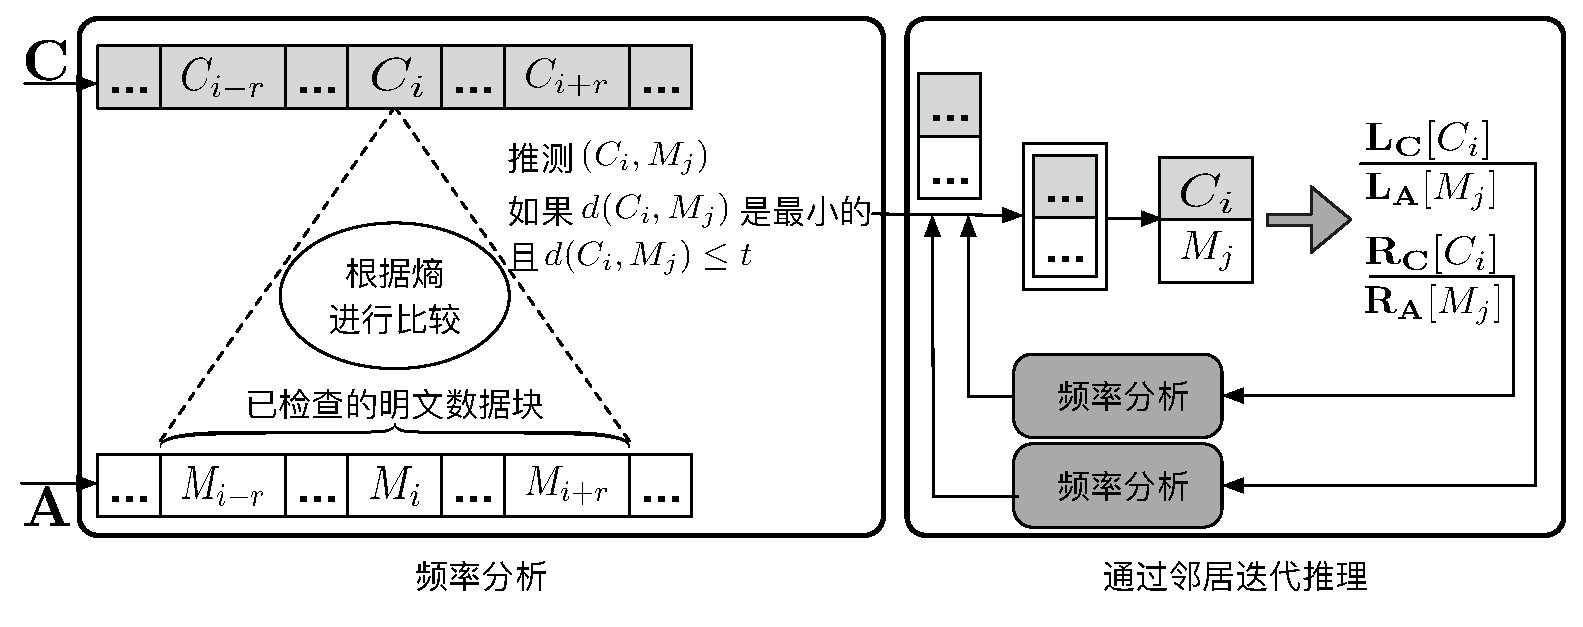
\includegraphics[width=14cm]{DistributionAttack}
    \caption{基于分布的频率分析攻击工作流程} 
    \label{fig:基于分布的频率分析攻击工作流程}
\end{figure}

图\ref{fig:基于分布的频率分析攻击工作流程}展示了基于分布的频率分析攻击方案的工作流程。

首先按$\mathbf{C}$和$\mathbf{A}$中的频率对具有唯一性的密文和明文进行排序。 与基于数据块局部性的频率分析攻击\citing{li2017information}一样,通过参数$u$将基础频率分析配置为最多返回$u$个频率最高的明密文数据块对。

接下来,对于每个具有唯一性的密文数据块$C_i$(其中$i, 1 \leq i \leq u$,代表了该密文数据块的频率排名),检查相近频率排名范围内明文数据块$M_{i-r}, \ldots, M_i, \ldots, M_{i+r}$(从$i-r$到$i+r$),其中$r$是可配置参数(默认为10),表示可以解决的频率排名干扰的最大范围。

对于每个$C_i$(其中$1 \leq i \leq u$)和相应的$M_j$(其中$i-r\le j\le i+r$),我们通过熵来表示它们的相对频率分布,熵是信息理论中的一个关键概念,用于衡量随机来源产生的信息量。在这里,我们采用熵来量化概率分布的随机性\citing{wang08}。 具体来说,我们定义了两个随机变量,分别用$X$和$Y$来描述$C_i$与其左右邻居的共现事件,这样事件“$X = C$” 表示$C$是$C_i$的左邻居,而事件$Y = C$表示$C$是$C_i$的右邻居。 因此,我们基于$\mathbf{L_C}$和$\mathbf{R_C}$来计算两个事件发生的概率:
\begin{equation}
\begin{aligned}
\label{eq:PrXYdis}
    \Pr[X = C] &=& \frac{\mathbf{L_C}[C_i][C]}{\sum_{C' \in \mathbf{L_C}[C_i]} \mathbf{L_C}[C_i][C']},  \\
    \Pr[Y = C] &=& \frac{\mathbf{R_C}[C_i][C]}{\sum_{C' \in \mathbf{R_C}[C_i]} \mathbf{R_C}[C_i][C']}, 
\end{aligned}
\end{equation}

其中$\mathbf{L_C}[C_i]$和$\mathbf{R_C}[C_i]$分别了存储$C_i$的左右邻居,而$\mathbf{L_C}[C_i][C']$和$\mathbf{R_C}[C_i][C']$存储$C_i$与其左右邻居$C'$的共现频率。$X$和$Y$都遵循$C_i$的相对频率分布,本文用$e(\mathbf{L_C}[C_i])$和$e(\mathbf{R_C}[C_i])$表征它们的随机性,分别为:

\begin{equation}
\begin{aligned}
\label{eq:e-dis}
    e(\mathbf{L_C}[C_i]) &=& \sum_{C \in \mathbf{L_C}[C_i]} \log_2\frac{1}{\Pr[X = C]}, \\
    e(\mathbf{R_C}[C_i]) &=& \sum_{C \in \mathbf{R_C}[C_i]} \log_2\frac{1}{\Pr[Y = C]}. 
\end{aligned}
\end{equation}

类似的,本文根据$\mathbf{L_A}$和$\mathbf{R_A}$对每个明文数据块$M_j$(其中$i-r\le j\le i+r$)计算出其对应的熵$e(\mathbf{L_A}[M_j])$和$e(\mathbf{R_A}[M_j])$,然后本文利用欧几里得距离来量化$C_i$和$M_j$的相对频率分布的相似性,记为$d(C_i, M_j)$:

\begin{equation}
    \label{eq:dis-dcm}
    \centering
    d(C_i, M_j) = \sqrt{[e(\mathbf{L_C}[C_i]) - e(\mathbf{L_A}[M_j])]^2 + [e(\mathbf{R_C}[C_i]) - e(\mathbf{R_A}[M_j])]^2}.
\end{equation}

显然,只有当他们的熵的欧几里德距离$d(C_i, M_j)$很小时,$C_i$和$M_j$才有相似的相对频率分布。因此,如果满足以下条件,则可将$(C_i, M_j)$标识为推理成功的密文数据块-明文数据块对:

\begin{itemize}
\item \textbf{R1:} $d(C_i, M_j)$ 在$j \in i-r \leq j \leq i+r$ 中取到最小值。
\item \textbf{R2:} $d(C_i, M_j)$ 不大于预先设定的变量$t$(例如,$t$的默认值为1)。
\end{itemize}

值得注意的是,$C_i$所对应的原始明文数据块可能不在检查的明文数据块$M_{i-r}, \ldots, M_{i+r}$的范围内。在这种情况下,部分$M_j$($i-r \leq j \leq i+r$)可能仍然满足条件R1。这种情况下,本文希望通过R2过滤不正确的密文数据块-明文数据块对。 

然后,继续采用先前基于数据块局部性的频率分析攻击\citing{li2017information}中的迭代方法(参见章节:\ref{sec:DistributionAttack-prior-attack})来扩展推理的密文数据块-明文数据块对的覆盖范围。具体来说,对于每个推理的$(C_i, M_j)$,应用基于分布的频率分析方案(见上文)通过$C_i$和$M_j$的邻居迭代推理出更多的密文数据块-明文数据块对,在没有新的密文数据块-明文数据块对可以被推理时停止迭代,最终完成基于分布的频率分析攻击的全部过程。
 
\subsection{基于分布的频率分析攻击方法总结} 

总而言之,基于分布的频率分析攻击通过在频率分析中考虑相对频率分布来提供更一般化的局部性概念。它通过三个参数进行配置和调整:

\begin{itemize}
    \item $u$:确定通过频率分析返回的密文数据块-明文数据块对的最大数量。
    \item $r$:确定要考虑的扰动范围的最大值。
    \item $t$:确定欧几里德距离的阈值以过滤可能不正确的推理结果。 
\end{itemize}


先前基于数据块局部性的频率分析攻击\citing{li2017information}可以被视为基于分布的频率分析攻击在$r=0$的参数配置下(即没有处理频率排名中的任何干扰)和$t \rightarrow \infty$(即没有过滤任何不正确的推理结果)的特殊情况。

\section{对数据块大小信息泄漏的利用}

本文提出了基于分布的频率分析攻击的高级变体,它使用数据块大小信息来进一步减少误报。具体来说,假设$\mathbf{C}$中每个密文数据块的大小反映了其原始明文数据块的大小。 

本文的想法建立在这样一个基本事实的基础上:如果密文$C$对应于明文$M$,则$C$的大小近似于$M$的大小。 这是因为加密重复数据删除在要加密的内容中保留了块(即,由对称加密操作的基本单元)的数量信息。 本文通过使用这个事实来进一步过滤不正确的密文数据块-明文数据块对$(C,M)$($C$和$M$中的块数不同)。

在本课题中,假设每个块的大小都是16字节(AES加密的典型配置)。对于每个经过基于分布的频率分析攻击方法得到的明文数据块-密文数据块对$(C_i, M_j)$,分别将$C_i$和$M_j$中的块数导出为$b({C_i})$和$b({M_j})$:

\begin{equation}
\begin{aligned}
\label{eq:b-dis}
b({C_i}) = \lceil \frac{{\sf size}(C_i)}{16} \rceil,  \\
b({M_j}) = \lceil \frac{{\sf size}(M_j)}{16} \rceil, 
\end{aligned}
\end{equation}

其中${\sf size}(C_i)$和${\sf size}(M_j)$分别是$C_i$和$M_j$的确切大小, $\lceil x \rceil$ 返回了大于或等于$x$的最小整数。在基于分布的频率分析攻击中提出的过滤条件R1和R2(参见章节:\ref{sec:distribution-attack-description})的基础上,给出以下过基于数据块中块数信息的滤条件:  
 
\begin{itemize}[leftmargin=*]
    \item {\bf R3:} $b({C_i})$ equals $b({M_j})$.
\end{itemize}

对于使用可变大小的数据分块方法的加密重复数据删除中,不同的数据块可能具有不同的大小,因此使用R3可以有效进行过滤。然而,在使用固定大小的数据分块方法的机密重复数据删除中,R3对于任意一组$(C, M)$始终成立。但此时,仍然可以通过应用R1和R2来提高频率分析攻击的精度。
     

\section{本章小结}

本章介绍了本文提出的第一种改进的频率分析方法:基于分布的频率分析攻击方法。给出了该方法的形式定义、方法描述以及对数据块大小信息泄漏的扩展利用方法。                  




\chapter{基于聚类的频率分析攻击方法}
\label{sec:ClusteringAttack}

本章放松了基于分布的频率分析攻击中的攻击者的攻击条件要求,提出了基于聚类的频率分析攻击,它不需要使用明文数据块的细粒度排序信息。相反,它利用相似性这一属性来推理来自相似的数据段(即,由数据块块聚合形成的更大的数据单元)的原始数据块,而不依赖于每个数据段中的数据块的排序。 本章首先介绍相似性的概念,然后展示如何使该属性进行推理攻击。

\section{背景知识}
\label{sec:similarity}

\subsection{min-wise independence条件}

对于min-wise independence置换族\citing{broder2000min}有如下定义:设$S_n$是$n$元集合$[n]$上所有置换组成的n元对称群。称置换族$F \subseteq S_n$满足min-wise independence条件是指:对任意$X=\{x_1,x_2,\cdots,x_m\}\in[n]$和任意$x_i-inX$,从集合$F$中随机、均匀地选取函数$h$,计算$H(X)=\{h(x_1),h(x_2),\cdots,h(x_m),\}$,有下式成立:
\begin{equation}
    \label{eq:min-wise independence}
    Pr(min(H(X)) = h(x_i) ) = \frac{1}{|X|}
\end{equation}

即$X$中的所有元素在$h$的作用下都有相等的概率成为$H(X)$中的最小元。在实际应用中,完全满足min-wise independence条件的哈希函数很难实现,通常使用近似满足min-wise independence条件\citing{broder2000min}的哈希函数即可。

\subsection{Broder定理}
Broder定理\citing{broder1997resemblance}的定义为:两集合$S_1$和$S_2$,$H(S_i)=\{h(x_k)|\forall x_k \in S_i \}$,h是满足min-wise independence条件的哈希函数,$min(S_i)$代表集合$S_i$中的最小元,则

\begin{equation}
    \label{eq:broder}
    \Pr[\min\{{\rm H}(S_1)\} = \min\{{\rm H}(S_2)\} ] = \frac{|S_1 \cap S_2|}{|S_1 \cup S_2|}
\end{equation}

\subsection{相似性}
相似性\citing{bhagwat2009extreme}指出来自同一来源的备份文件可能类似并且共享大部分相同的数据块。 备份文件之间的相似性可以通过Broder定理\citing{broder1997resemblance}来量化。具体来说,如果将每个文件视为一个数据块的集合$S$(即忽略它们的顺序),Broder定理指出如果两组数据块共享相同的最小数据块哈希值的概率很高,则两个集合包含的数据块可能大部分都相同,反之亦然:
 
\begin{equation}
	\Pr[\min\{{\rm H}(S)\} = \min\{{\rm H}(S')\} ] = \frac{|S \cap S'|}{|S \cup S'|}
	\label{eq:similary}
\end{equation}

其中${\rm H}(\cdot)$是一个从min-wise independence置换族中随机统一选择的哈希函数,$\min\{{\rm H}(S)\}$是$S$的最小数据块的哈希。为了便于描述,本文使用MinHash来表示集合中元素的最小哈希值。


针对重复数据删除的各个方面(性能方面\citing{qin2017design,xia2011silo,bhagwat2009extreme},安全方面\citing{li2017information})的已有工作已经利用了相似性这一属性来保持存储效率。具体来说,它们仅针对共享相同最小数据块哈希的文件(即类似的文件)采用MinHash作为一个数据块集合中所有数据块加密使用的密钥进行重复数据删除。根据Broder定理可以推理得到这类文件可能具有大量相同的数据块,因此这种近似精确的重复数据删除只会导致存储效率的轻微降低。与先前的方法不同\citing{qin2017design,xia2011silo,bhagwat2009extreme,li2017information},本文应用相似性来提高频率分析攻击的有效性。
 
\section{基于聚类的频率分析攻击方法定义}
\label{sec:clustering-attack-description}

现在提出基于聚类的频率分析攻击方法(图:\ref{fig:基于聚类的攻击方法的工作流程}),它基于相似性在加密重复数据删除中推理密文数据块的原始明文数据块。

\begin{figure}[!htb]
    \small
    \centering
    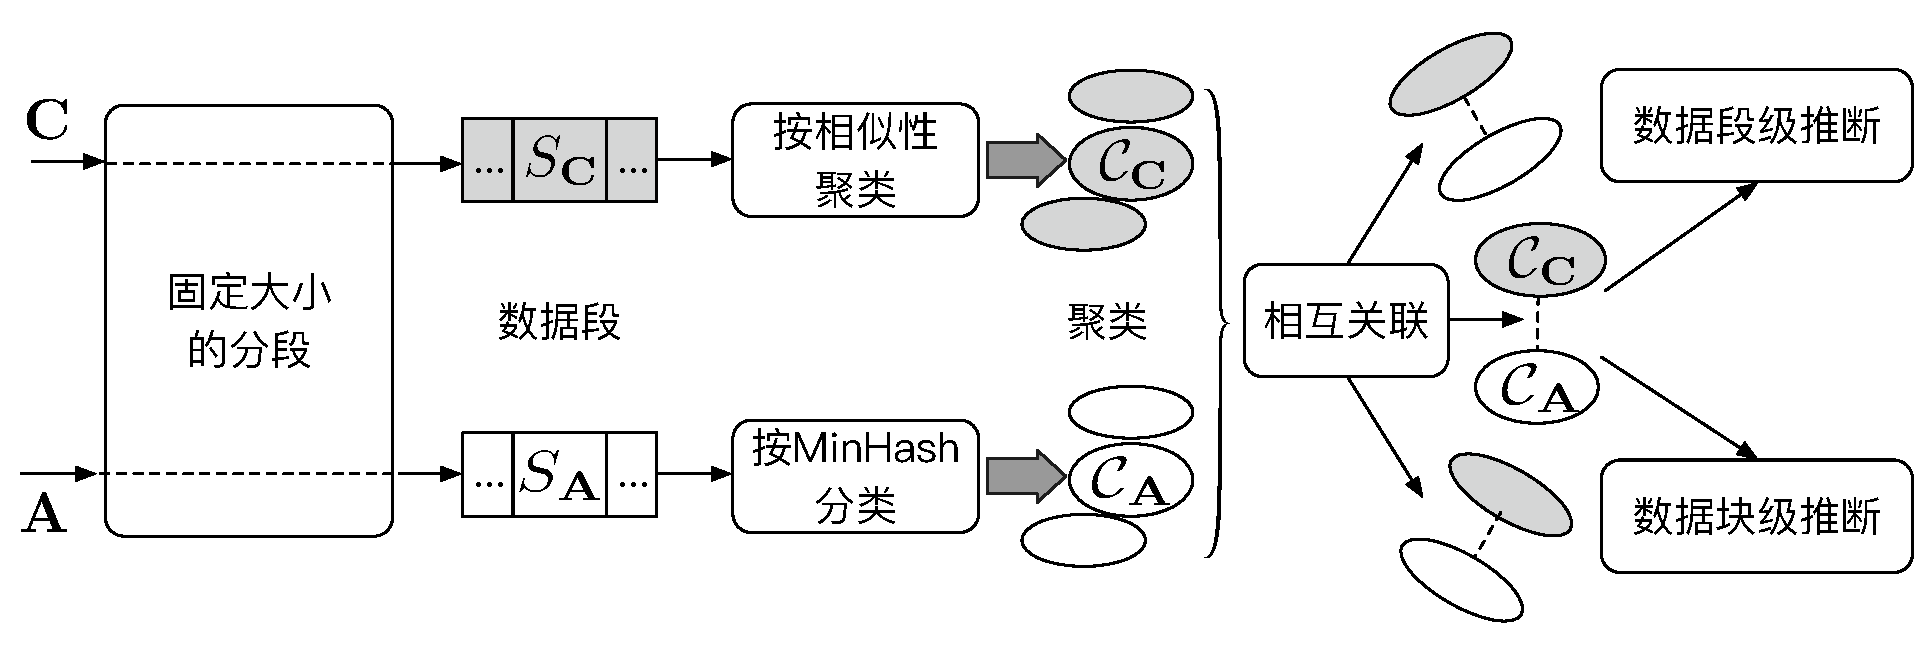
\includegraphics[width=14cm]{ClusteringAttack.eps}
    \caption{基于聚类的攻击方法的工作流程:用MinHash表示明文数据段的最小块散列} 
    \label{fig:基于聚类的攻击方法的工作流程}
\end{figure}

为了利用相似,本文首先在数据块概念的基础上引入数据段的概念。具体来说,将$\mathbf{C}$划分为为一些粗粒度的数据单元,成为密文数据段。密文数据段使用$S_\mathbf{C}$来表示,其中包含有$\mathbf{C}$中的多个相邻的密文数据块。在本课题中,应用了定长分段方法,以确保每个数据段具有相同分的大小(例如,默认大小为4MB)。同样的,对于攻击者所具有的辅助信息$\mathbf{A}$,也同样使用定长分段方法产生多个明文数据段,每个数据段由$S_\mathbf{A}$表示。

注意,一些可变大小的分段方案\citing{lillibridge2009sparse,qin2017design}在其内容与特定模式匹配的数据块之后设置分段边界,从而解决固定大小分段方案所面临的边界移位问题。但是,本文不能在攻击中使用这些可变大小的分段方案\citing{lillibridge2009sparse,qin2017design}。其原因是密文数据段中的数据块的原始内容受到对称加密的保护,攻击者无法确保密文和明文数据段的边界匹配采用的是相同的模式。该问题会导致密文和明文数据段不兼容,从而会降低基于聚类的攻击方法所推理的数据段级的数据量(请参阅本章后半部分)。
 
本方法通过类似的数据段来推理密文-明文对。给出$S_\mathbf{M}$是对应于密文数据段$S_\mathbf{C}$的明文数据段(即$S_\mathbf{M}$中的每个明文数据块对应于$S_\mathbf{C}$中的某些密文数据块,反之亦然)。根据Broder定理,如果一个明文数据段$S_\mathbf{M}$与辅助信息中的明文数据段$S_\mathbf{A}$具有相同的最小数据块哈希(称为$h$),则$S_\mathbf{M}$和$S_\mathbf{A}$可能拥有拥有大量相同的明文数据块。这意味着$S_\mathbf{C}$中的密文数据块很可能是从$S_\mathbf{A}$中的明文数据块映射得到的。换言之,攻击者首先按照最小数据块哈希对$\mathbf{A}$中的所有明文数据段进行分类,以此获得多个明文数据段集合(聚类的不同类别)。将每个明文数据段集合用$\mathcal{C}_\mathbf{A} = \{ S_\mathbf{A} \}$表示,对应于该集合中包含的所有明文数据段共有的唯一最小数据块哈希。同理,攻击者将密文数据段也进行上述分类操作,对于每个分类的集合用$\mathcal{C}_\mathbf{C} = \{ S_\mathbf{C} \}$表示)。然后,攻击者从对应于某一最小数据块哈希$h$的$\mathcal{C}_\mathbf{A}$中推理出$\mathcal{C}_\mathbf{C}$的原始明文数据。  

在本文中,定义任意两个密文数据段$S_\mathbf{C}$和$S_\mathbf{C}'$的聚类距离$d(S_\mathbf{C},S_\mathbf{C}')$为1减去相同密文的分数:

\begin{equation}
\label{eq:distence}
    d(S_\mathbf{C}, S_\mathbf{C}') = 1 - \frac{|S_\mathbf{C} \cap S_\mathbf{C}'|}{|S_\mathbf{C} \cup S_\mathbf{C}'|}.
\end{equation}

在推理过程中,相同的密文可能会在$S_\mathbf{C}$或$S_\mathbf{C}'$中重复出现,而$|S_\mathbf{C} \cap S_\mathbf{C}'|$和$|S_\mathbf{C} \cup S_\mathbf{C}'|$ 会分别返回其交集和并集中具有唯一性的密文数据块的数量。显然,$d(S_\mathbf{C}, S_\mathbf{C}')$越小,则说明$S_\mathbf{C}$和$S_\mathbf{C}'$更可能对应相同的最小数据块哈希。在本章中,采用凝聚法层次聚类(AHC)\citing{johnson1967hierarchical}方法来根据距离信息聚合相似的密文数据段。具体来说,攻击者从其拥有的每个密文数据段开始,将每个密文数据段视为一个单独的聚类类别,然后计算各个聚类之间的距离,将两个距离最近的(最相似的)聚类合并在一起,不断迭代这一过程直到任意两个聚类间的距离均大于给定最大距离参数$k$时停止迭代操作。
 
对于最终得到的每个密文聚类$\mathcal{C}_\mathbf{C}$,攻击者在考虑频率分布的前提下通过频率分析将其与一些明文聚类$\mathcal{C}_\mathbf{A}$相关联。该操作方法基于如下观察:相同的密文数据段(明文数据段)可以在相同或不同的密文数据段(明文数据段)中重复出现,并且相同的密文(明文)数据段也可以在相同的密文(明文)聚类中重复出现。同时,攻击者检查每个聚类中明文数据块或密文数据块的频率分布,并且认为相似的聚类(即,对应于相同的最小数据块哈希)中数据块的频率分布也是相似的。
 
本文按如下的顺序来设计频率分析攻击方案。首先,将所有可用的密文和明文聚类分别按它们包含的逻辑密文数据块和明文数据块的总数进行排序。然后,计算一个关联数组$\mathbf{F}$用于存储相应聚类中每个具有唯一性的密文数据块或明文数据块的频率。基于 $\mathbf{F}$,计算密文数据块$C$存在于密文聚类$\mathcal{C}_\mathbf{C}$中的概率$\Pr[C \in \mathcal{C}_\mathbf{C}]$,并进一步计算$\mathcal{C}_\mathbf{C}$的熵$e(\mathcal{C}_\mathbf{C})$:     

\begin{equation}
\begin{aligned}
\label{eq:Pr&eincluster}
    \Pr[C \in \mathcal{C}_\mathbf{C}] &= \frac{\mathbf{F}[\mathcal{C}_\mathbf{C}][C]}{\sum_{C' \in \mathcal{C}_\mathbf{C}} \mathbf{F}[\mathcal{C}_\mathbf{C}][C']} \\
    e(\mathcal{C}_\mathbf{C}) &= \sum_{C \in \mathcal{C}_\mathbf{C}} \log_2 \frac{1}{\Pr[C \in \mathcal{C}_\mathbf{C}]} 
\end{aligned}
\end{equation}

其中$\mathbf{F}[\mathcal{C}_\mathbf{C}][C]$存储了$\mathcal{C}_\mathbf{C}$中密文数据块$C$的频率。同理,计算出明文聚类$\mathcal{C}_\mathbf{A}$的熵$e(\mathcal{C}_\mathbf{A})$。与基于分布的频率分析攻击(参见\ref{sec:distribution-attack-description})类似,本文使用参数$(u, r, t)$来配置频率分析攻击方案。如果密文聚类$\mathcal{C}_\mathbf{C}$和明文聚类$\mathcal{C}_\mathbf{A}$满足如下三个条件则可说明两个聚类相似:   


\begin{itemize}
    \item  $\mathcal{C}_\mathbf{C}$的排名数值大小不大于$u$。
    \item  $\mathcal{C}_\mathbf{C}$和$\mathcal{C}_\mathbf{A}$的排名数值差距大小不大于$r$。  
    \item  $e(\mathcal{C}_\mathbf{C})$和$e(\mathcal{C}_\mathbf{A})$的差异是最小的,且不超过$t$.
\end{itemize}

然后,对于每个相似的聚类对$(\mathcal{C}_\mathbf{C}, \mathcal{C}_\mathbf{A})$,攻击者在两个级别分别进行明密文对的推理工作。

\begin{itemize}
    \item \textbf{数据段级推理}
    
    \par 如果$\mathcal{C}_\mathbf{C}$和$\mathcal{C}_\mathbf{A}$拥有相同数量的逻辑数据块(即密文数据块或明文数据块)以及相同的熵,则$\mathcal{C}_\mathbf{C}$与$\mathcal{C}_\mathbf{A}$完全映射的概率很高。在这种情况下,攻击者对粗粒度的数据段进行攻击。具体来说,攻击者首先在$\mathcal{C}_\mathbf{C}$中基于其密文的频率分布计算每个密文数据段$S_\mathbf{C}$的熵,并在$\mathcal{C}_\mathbf{A}$中基于其明文的频率分布计算每个明文数据段$S_\mathbf{A}$的熵。
         
         
    \par 如果$S_\mathbf{C}$和$S_\mathbf{A}$中逻辑数据块的总数和熵一致,则攻击者可以推理密文数据段$S_\mathbf{C}$是由命文数据段$S_\mathbf{A}$映射得到的。根据实验表明,基于聚类的频率分析攻击中大部分推理正确的内容来自于数据段级推理。同时,攻击者还可以利用额外的对抗性知识(例如,逻辑块顺序)来进一步恢复这些推理出的数据段中的每个数据块的明文。
         
    \item \textbf{数据块级推理}
    
    
    \par 如果$\mathcal{C}_\mathbf{C}$和$\mathcal{C}_\mathbf{A}$中具有的逻辑块数量或熵不同,攻击者对细粒度的数据块进行攻击。具体来说,攻击者分别对$\mathcal{C}_\mathbf{C}$和$\mathcal{C}_\mathbf{A}$中的具有唯一性的密文数据块和明文数据块按照出现频率进行排序,以此根据频率排名的顺序推理明文数据块-密文数据块对。            
     
    \par 然而,实验发现数据块级推理在本文给出的实验数据集中表现不佳。可能的原因是每个聚类包括大量逻辑数据块,这降低了频率分析的有效性。但即便如此,本文预计数据块级推理可以在实践中正确推理出更多的密文数据块-明文数据块对,当某些聚类中的逻辑数据块数量有限时效果会更佳。
 
\end{itemize}

\subsection{基于聚类的频率分析攻击方法总结}

总而言之,基于聚类的频率分析攻击利用相似性,在类似的聚类类别中使用频率分析攻击以推理密文数据块-明文数据块对。 除$u$,$r$和$t$外,它还由参数$k$配置,该参数指定了配对两个聚类类别的距离上限。

尽管可能受到固定大小数据段的边界偏移问题的影响,但本文认为基于聚类的频率分析攻击对VM磁盘映像的攻击效果是显著的。VM映像文件在创建时被分配了固定的大小,并且在其生存期内无法改变。在开始写入数据前,VM映像中的所有空间均由全零数据进行填充。在将数据存入映像的过程中,通过将需要用到的部分空间进行重写来完成数据存入过程。在章节\ref{sec:experiment-clustering}中,本文研究了针对VM磁盘映像的基于聚类的频率分析攻击的有效性。

\section{本章小结}

本章介绍了本文提出的第二种改进的频率分析方法:基于聚类的频率分析攻击方法。给出了该方法的相关背景知识、形式定义、方法描述以及最佳的适用场景。                  



\chapter{数据集与实际系统调研}
\label{sec:DataSetSystem}
\section{数据集调研}

本文调研与使用以下数据集用于评估提出的两种攻击方法的效果,通过模拟攻击评估重复数据删除中信息泄漏带来的安全隐患(参见\ref{sec:background})。

\subsection{FSL数据集}
\label{sec:fsl}
\begin{table}[!hbt]
    \caption{FSL数据集特征}
\small
\label{tab:FSL-dataset}
\centering
\begin{tabular}{|c|c|c|c|}
\hline
\multirow{2}{*}{\bf 类别} & \multicolumn{3}{c|}{\bf 备份中的特征} \\
\cline{2-4}
    & \#逻辑数据块数(百万) & \#唯一数据块数(百万) & 近似逻辑大小(GB)\\
\hline
User004  & 1.0-1.3 & 0.7-0.9 & 10GB/备份$\times$ 14个\\
\cline{1-4}
User007 &  3.5-5.2 & 2.3-3.6 & 39GB/备份 $\times$ 14个\\
\cline{1-4}
User012 &  25.0-26.4 & 8.9-9.7 & 244GB/备份 $\times$ 14个\\
\cline{1-4}
User013 &  1.8-5.7 & 1.2-4.2 & 22GB/备份 $\times$ 14个\\
\cline{1-4}
User015 &  13.4-20.5 & 9.0-11.0 & 158GB/备份 $\times$ 14个\\
\cline{1-4}
User028 &  6.0-10.3 & 3.5-6.8 & 77GB/备份 $\times$ 14个\\
\hline
\end{tabular}
\end{table}

表\ref{tab:FSL-dataset}总结了FSL实验数据集的相关特征信息,其中\#逻辑数据块数 和 \#唯一数据块数表示每个实验快照中逻辑数据块数量和具有唯一性的数据块数量。

此数据集由Stony Brook大学的文件系统和存储实验室(FSL)收集\citing{sun2016long,FSL14,sun2018cluster}。本文使用fslhomes快照进行实验,每个快照包括48位数据块哈希的有序列表,这些哈希是由平均大小为8KB的可变大小分块生成的,以及相应的元数据信息(例如,数据块大小、文件名、扩展名等)。本文从2013年1月22日到5月21日选择快照,并选择在整个持续时间内具有完整每日快照的六个用户(即User004,User007,User012,User013,User015和User028)用于后续实验分析。本文以周为单位选取备份数据,因此为每个用户选出14个每周完整备份。

\subsection{VM数据集}
\label{sec:vm}
\begin{table}[!hbt]
    \caption{VM数据集特征}
\small
\label{tab:VM-dataset}
\renewcommand{\arraystretch}{1.2}
\vspace{-3pt}
\centering
\begin{tabular}{|c|c|c|c|}
\hline
\multirow{2}{*}{\bf 类别} & \multicolumn{3}{c|}{\bf 备份中的特征} \\
\cline{2-4}
    & \#逻辑数据块数(百万) & \#唯一数据块数(百万) & 近似逻辑大小(GB)\\

\hline
User1  &  \multirow{6}{*}{2.6} & $\sim$0.9 & 25GB/备份 $\times$ 13 个 \\
\cline{1-1}
\cline{3-4}
User2 &  & 1.1-1.3 & 28GB/备份 $\times$ 13 个\\
\cline{1-1}
\cline{3-4}
User3 &  & 0.9-1.1 & 26GB/备份 $\times$ 13 个\\
\cline{1-1}
\cline{3-4}
User4 &  & $\sim$0.9 & 25GB/备份 $\times$ 13 个\\
\cline{1-1}
\cline{3-4}
User5 &  & 0.9-1.0 & 25GB/备份 $\times$ 13 个\\
\cline{1-1}
\cline{3-4}
User6 &  & 0.9-1.1 & 27GB/备份 $\times$ 13 个\\
\hline
\end{tabular} 
\end{table}

表\ref{tab:VM-dataset}总结了VM实验数据集的相关特征信息,其中\#逻辑数据块数 和 \#唯一数据块数表示每个实验快照中逻辑数据块数量和具有唯一性的数据块数量。由于所有的VM映像都具有10GB的固定大小,因此其具有相同数量的逻辑块。。

此数据集是从某大学2014年春季的编程课程中收集的。原始数据集包括为课程中注册的学生提供的大量VM镜像快照,每个快照的大小固定为10GB,每个快照中的数据用固定大小为4KB的数据块通过SHA-1算法计算得到的哈希的列表表示。本文使用6个用户(即User1-User6)的数据,每个用户的数据由13个每周备份组成。

\subsection{MS数据集}
\label{sec:ubc-ms}
\begin{table}[!hbt]
    \caption{MS数据集特征}
\small
\label{tab:MS-dataset}
\renewcommand{\arraystretch}{1.2}
\vspace{-3pt}
\centering
\begin{tabular}{|c|c|c|c|}
\hline
\multirow{2}{*}{\bf 类别} & \multicolumn{3}{c|}{\bf 备份中的特征} \\
\cline{2-4}
    & \#逻辑数据块数(百万) & \#唯一数据块数(百万) & 近似逻辑大小(GB)\\

\hline
Win7  & 61.6-61.8 & 61.1-61.3 & 425GB/备份 $\times$ 4 个\\
\cline{1-4}
Serv-03 & 10.6-10.7 & 8.4-8.5 & 78GB/备份 $\times$ 4 个\\
\cline{1-4}
Serv-08 & $\sim$6.5 & $\sim$3.8 & 48GB/备份 $\times$ 4 个\\
\cline{1-4}
Vista-B &  $\sim$7.6 & $\sim$2.0 & 55GB/备份 $\times$ 4 个\\
\cline{1-4}
Vista-U &  $\sim$21.0 & $\sim$10.4 & 159GB/备份 $\times$ 4 个\\
\hline
\end{tabular}
\end{table}

表\ref{tab:MS-dataset}总结了MS实验数据集的相关特征信息,其中\#逻辑数据块数 和 \#唯一数据块数表示每个实验快照中逻辑数据块数量和具有唯一性的数据块数量。

此数据集由Microsoft\citing{meyer2012study}收集,并在SNIA\citing{ms}上公布。 原始数据集包含2009年9月5日至10月31日的Windows文件系统快照。每个快照由通过Rabin Fingerprinting\citing{rabin1981fingerprinting}获得的不同平均大小的40位数据块哈希表示。 本文使用以下类别的操作系统快照用于试验:Windows 7(Win7),Microsoft Windows Server 2003(Serv-03),Microsoft Windows Server 2008(Serv-08),Microsoft Windows Vista Business Edition( Vista-B)和Microsoft Windows Vista Ultimate Edition(Vista-U)。在每个类别中,选择四个快照(这些快照的平均数据块大小为8KB。 


\section{实际系统调研}
\subsection{SDFS}

SDFS\citing{SDFS}是一种分布式、可扩展的文件系统,旨在为应用程序提供具有较强灵活性的内联重复数据删除。该系统有两种部署方法:

\begin{itemize}
    \item \textbf{单节点配置}:实际运行时将数据存储在本地文件系统中。
    \item \textbf{多节点配置}:实际运行中将数据存储在远端存储服务商/服务器中。
\end{itemize}

\subsubsection{系统的整体结构}

\par SDFS系统的整体结构如下所示:

\begin{figure}[!htb]
    \small
    \centering
    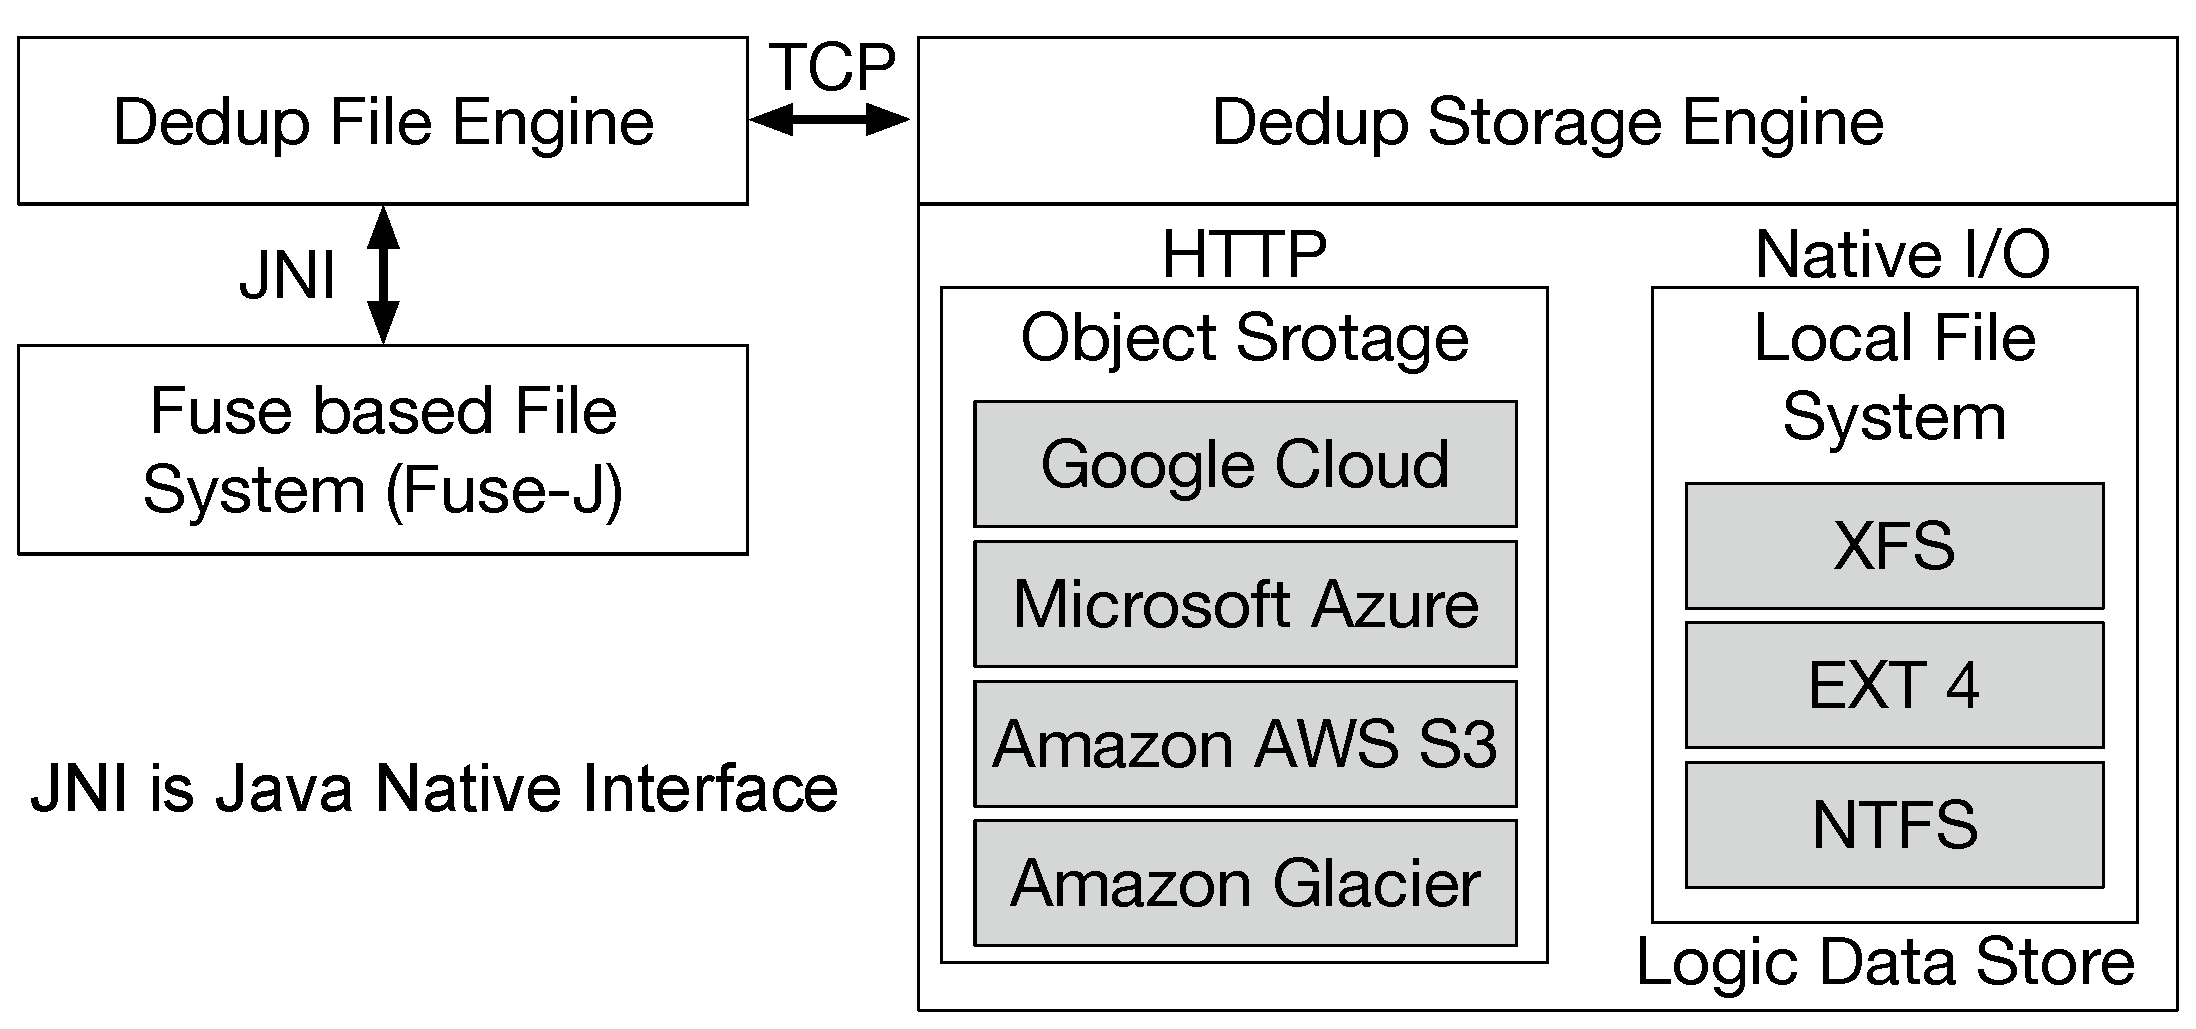
\includegraphics[width=11cm]{SDFS-Workflow}
    \caption{SDFS文件系统的运作流程} 
    \label{fig:SDFS-Workflow}
\end{figure}


该系统主要由以下四部分组成,其中Dedup File Engine和Dedup Storage Engine是SDFS系统的主要组件:

\begin{itemize}
    \item \textbf{Fuse Based File System (Fuse-J)}
    \item \textbf{Dedup File Engine}
    \item \textbf{Dedup Storage Engine}
    \item \textbf{Logic Data Store}
\end{itemize}


\subsubsection{Dedup File Engine}
本节将说明Dedup File Engine的工作原理以及相关的系统实现。Dedup File Engine的工作流程如下所示: 

\begin{figure}[!htb]
    \small
    \centering
    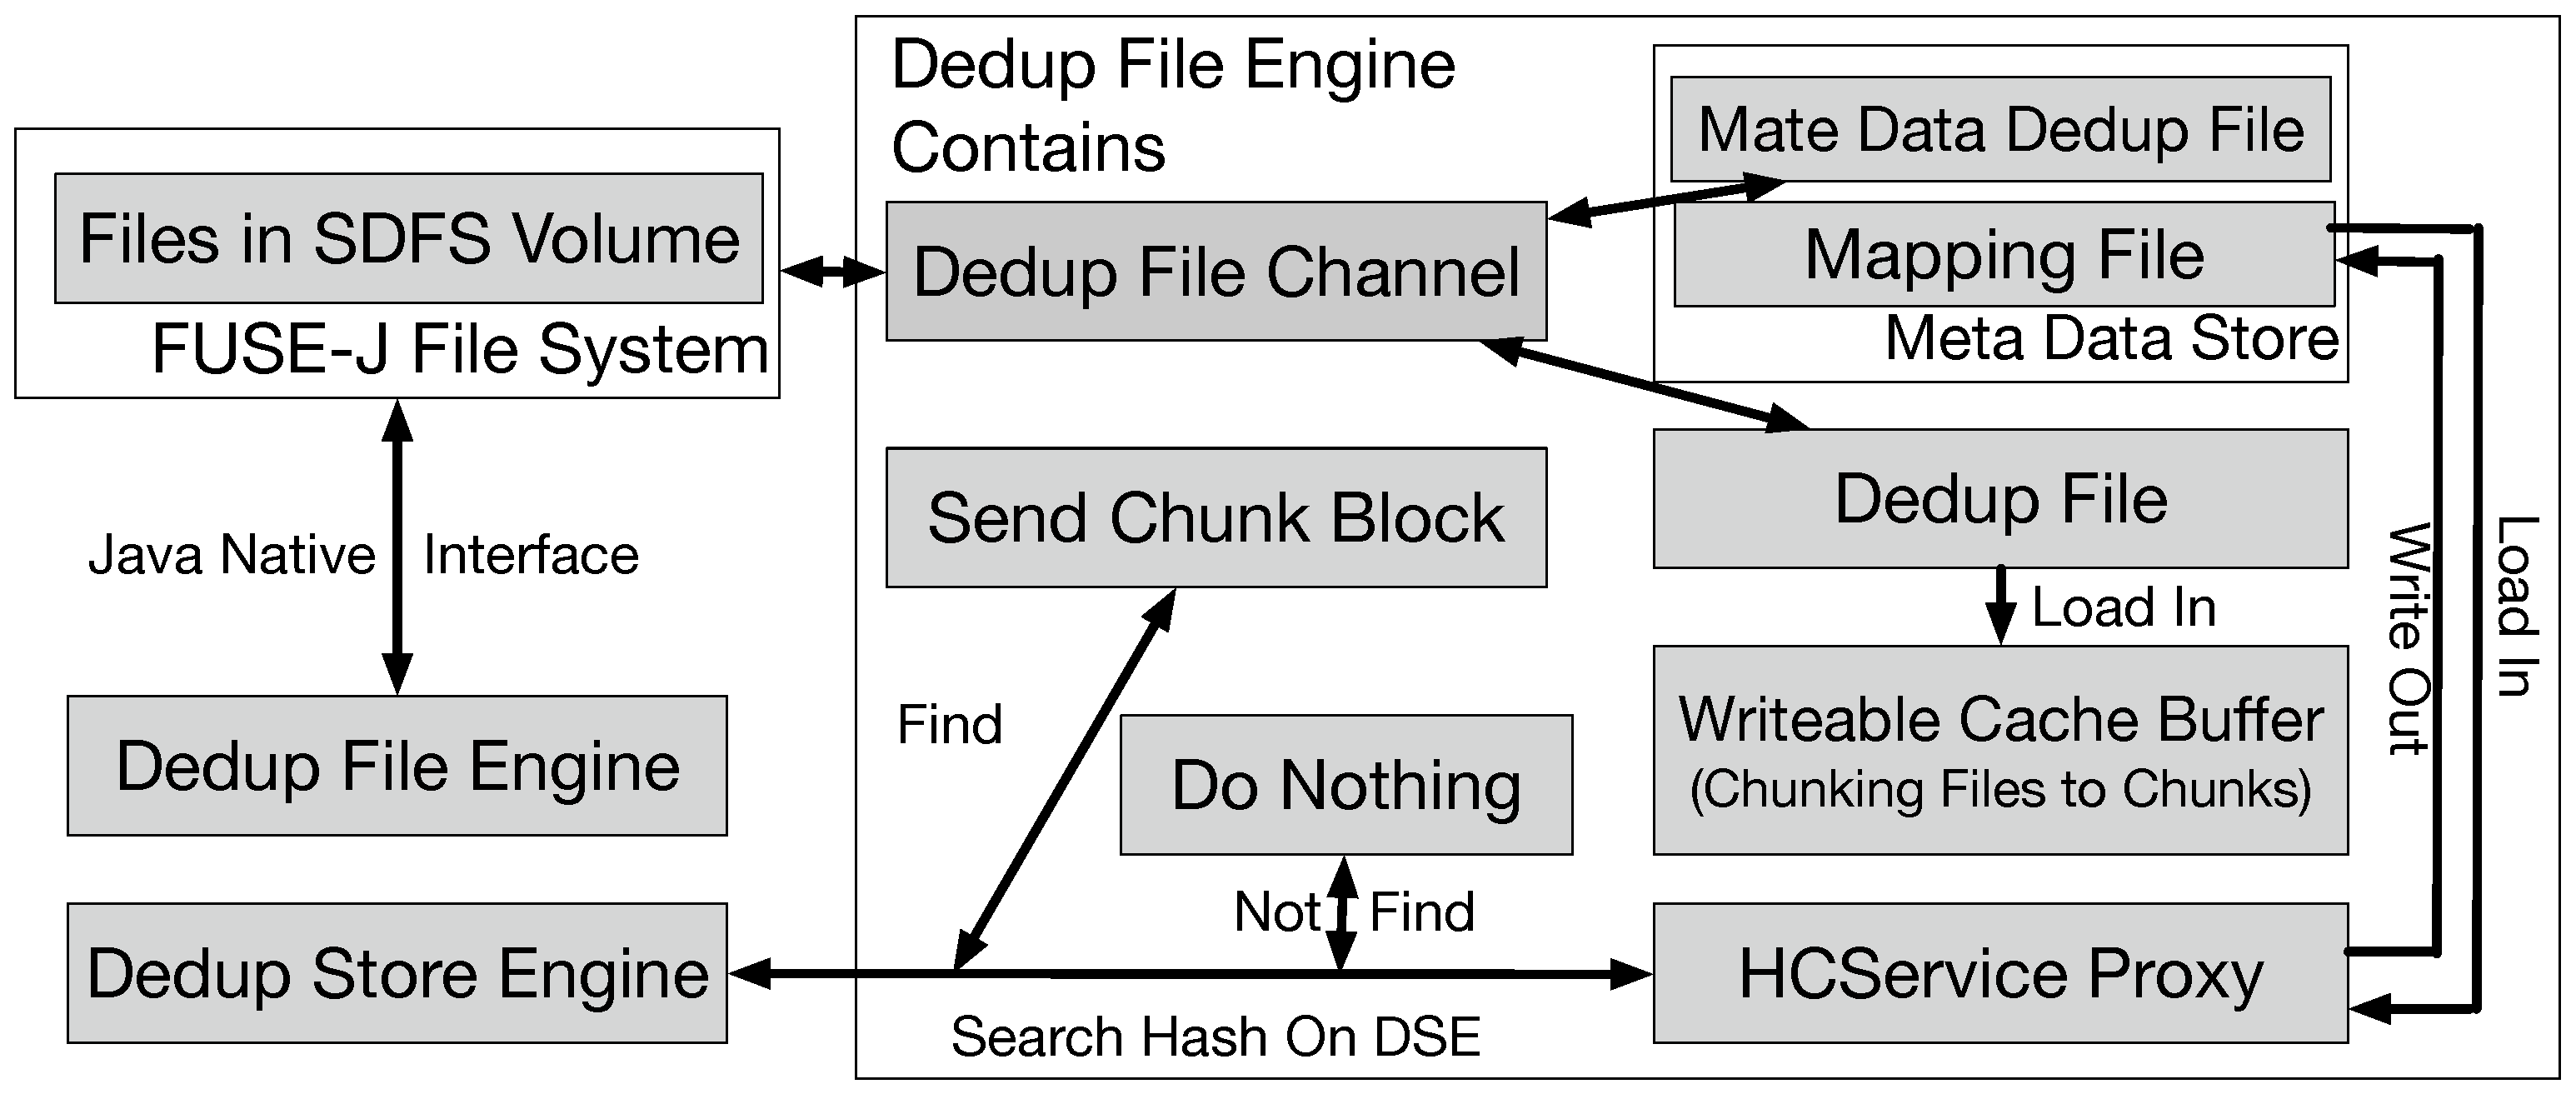
\includegraphics[width=11cm]{SDFS-DedupFileEngine.eps}
    \caption{SDFS文件系统的Dedup File Engine运作流程} 
    \label{fig:SDFS-DedupFileEngine}
\end{figure}

SDFS将Dedup File Engine通过Java Native Interface(JNI)连接到由FUSE-J驱动的实际文件系统的的卷,使得Dedup File Engine可以通过系统文件系统直接进行文件操作。

\textbf{Fuse-J Java Native Interface}

\begin{itemize}
    \item 文件统计和高级文件操作是通过获取和设置扩展文件属性(getfattr setfattr)来完成的。
    \item 每个挂载到SFDS的卷都拥有其独立的的Fuse-J接口和Dedup File Engine实例。
\end{itemize}

\textbf{Dedup File Channel}

本模块Fuse-J和DedupFile之间用于I/O命令的接口。该接口提供了一些方法(例如获取文件元数据/读取或写入文件)用于获取将进行重复数据删除的文件。

\textbf{Meta Data Store}


在SDFS文件系统中,文件通过两个不同的元数据进行表示,并将两种不同的元数据保存在两个不同的文件中。这两个文件分别为:

\begin{itemize}
    \item Meta Data Dedup File
    
    该文件用于存储进行重复数据删除的原始文件的文件属性元数据,包括文件大小、atime、ctime、acls以及指向关联映射文件的链接等。
    
    \item Mapping File

     该文件包含用于重复数据删除的文件的数据块记录列表,其存储了文件中每个数据块在原始文件中的位置、数据块是否具有唯一性、数据块的哈希值以及该数据块是否存储在远程服务器中。
\end{itemize}

\textbf{DedupFile}

该文件用于存储将要进行重复数据删除的文件的记录,其中的内容是挂载到SDFS文件系统的券中各个文件的哈希与完整文件路径与文件名的映射关系表。

\textbf{WritableCacheBuffer}

本数据结构包含一系列正在读取或写入的数据信息。在I/O活动期间,DedupFile会缓存其中的许多内容。在这部分中,SDFS使用SparseDedupFile类来处理writableCacheBuffer中的数据(即进行文件分块以获得获取逻辑数据块)。

SDFS支持两种数据块分块方法:固定大小的分块方法和Rabin可变大小数据块分块方法。

\textbf{HCService Proxy (HC == HashChunk)}

HCServiceProxy根据哈希的第一个字节(如果设置了多个Dedup Storage Engine)为当前数据块查找到适当的重复数据删除存储引擎。HCServiceProxy通过查询相应的Dedup File Engine以确定当前哈希所对应的数据块是否已存入存储系统(是否是重复的数据块),如果该数据块是重复的,则不进行任何操作,如果当前数据块是具有唯一性的,则将其加入存储系统中进行持久化存储。 


\subsubsection{Dedup Storage Engine}

Dedup Storage Engine(DSE)存储、检索和删除所有SDFS分割形成的数据块。重复数据删除存储引擎可以作为SDFS卷(单节点模式)的一部分运行,或在云端单独运行(多节点模式)。Dedup Storage Engine的运作流程如下所示: 

\begin{figure}[!htb]
    \small
    \centering
    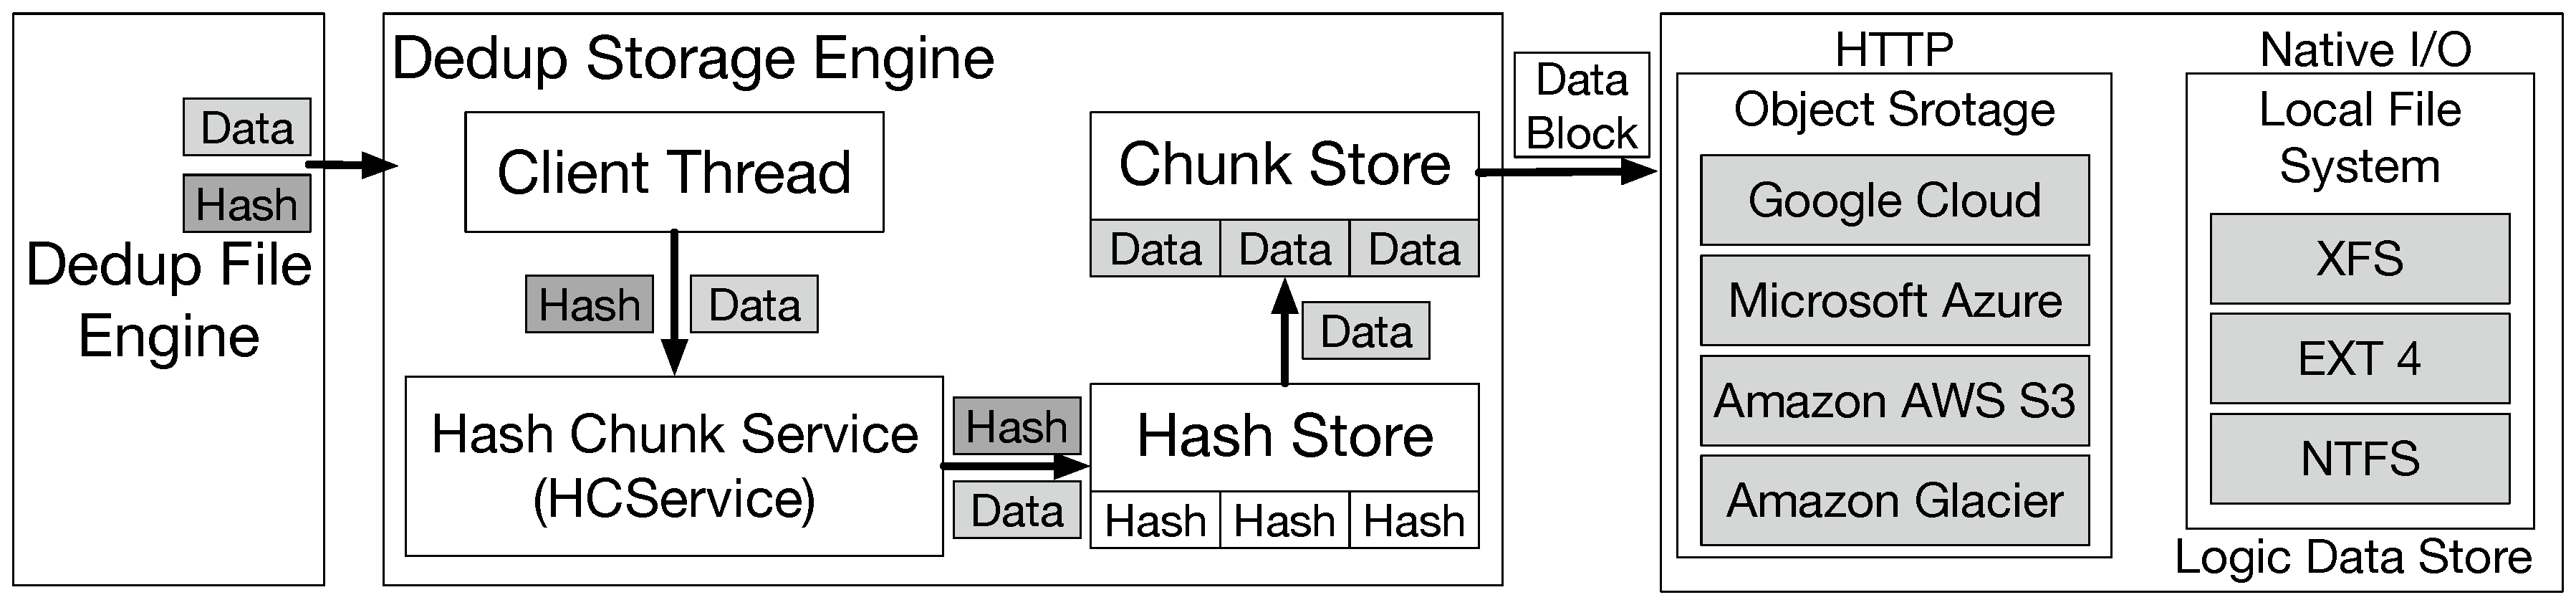
\includegraphics[width=\textwidth]{SDFS-DedupStorageEngine}
    \caption{SDFS文件系统的Dedup Storage Engine运作流程} 
    \label{fig:SDFS-DedupStorageEngine}
\end{figure}

\begin{enumerate}
    \item 客户端线程接收$WRITE\_HASH\_CMD$或$WRITE\_COMPRESSED\_CMD$信号并读取哈希和数据。
    \item 客户端线程将哈希传递给HashChunkService。
    \item HashChunkService将哈希和数据传递给适当的HashStore。
    \item HashStore存储哈希并将数据发送到指定的ChunkStore。
    \item ChunkStore存储数据。
\end{enumerate}

DES由2个基本组件组成:

\textbf{HashStore}

HashStore用于存储所有数据块的哈希与其对应的逻辑数据的存储位置。

\textbf{ChunkStore}

ChunkStore负责存储和检索与特定哈希相匹配的数据块原始逻辑数据。

\begin{itemize}
    \item 本地数据块存储
    \begin{itemize}
        \item 单文件数据块存储:将所有数据块写入一个文件中(文件大小与数据块总量有关)。
        \item 基于文件的数据块存储:将所有数据块依次写入固定大小的文件中。
    \end{itemize}
    \item 远程数据块存储
    \begin{itemize}
        \item Amazon S3
        \item Microsoft Azure
        \item Google Cloud
    \end{itemize}
\end{itemize}

\subsubsection{SDFS文件系统调研总结}

SDFS文件系统提供了商业使用级别的(加密)重复数据删除,但其中重复数据删除工作均先进行文件内的重复数据删除,再进行文件间的重复数据删除。其中的数据块处理顺序随机,不会发生数据块逻辑顺序信息的泄漏,因此可以防范本文提出的第一种攻击方法(基于分布的频率分析攻击方法)。但本文提出的第二种攻击手段在SDFS中仍然可以发挥作用。

\subsection{Destor}

Destor\citing{fu2015design}是重复数据删除的评估平台,其包含了大量重复数据删除中常用的方法,可以用于常用重复数据删除的方法测试与应用效果模拟评估。系统原型中包含的主要特征有:

\begin{itemize}
    \item 基于容器的数据块存储。
    \item 数据块级的管道通信。
    \item 三种重复数据删除方案:
    \begin{itemize}
        \item 基于固定大小的数据块分块的重复数据删除。
        \item 基于内容定义数据块分块方法的重复数据删除。
        \item 近似的文件级重复数据删除。
    \end{itemize}
    \item 多种文件重写算法:CFL、CBR、CAP和HAR等。
    \item 多种文件还原算法:LRU、最优替换算法和前滚组装。
\end{itemize}

\subsubsection{Destor系统原型调研总结}

Destor不同与商业化的SDFS文件系统,该系统原型是重复数据删除领域中著名的重复数据删除工具集合与样例。系统中的数据块处理是按照原有逻辑明文数据块的逻辑顺序进行的,因此会受到本文提出的两种攻击方法的威胁。

\section{本章小结}
本章介绍了本文用于评估攻击效果的三种真实世界数据集的来源和基本信息,以及两种现有重复数据删除系统的相关调研工作。

\chapter{实验测试与分析}
\label{sec:Experiment}

在本章中,将给出基于真实世界数据集的评估结果,以证明本文针对加密重复数据删除提出的频率分析攻击方法的有效性(对加密重复数据删除的威胁的严重性)。

\section{实验方法}
\label{sec:dataset}

本文所使用的真实世界数据集不包数据的实际内容,因此基于数据块哈希模拟攻击者所拥有的的对抗性知识。具体来说,本文将一些快照中的有序的数据块哈希列表作为辅助信息$\mathbf{A}$和原始明文信息$\mathbf{M}$。为了模拟加密过程,在$\mathbf{M}$中的每个原始数据块哈希(表示明文)上应用额外的哈希函数,并将结果截断为当前使用的数据集中约定的哈希值的长度。截断的结果用于模仿$\mathbf{C}$中的密文。对于每个推理的密文数据块-明文数据块对$(C,M)$,本文通过在$M$上应用相同的模拟加密并将结果与​​$C$进行比较来验证其正确性。特别的,基于聚类的频率分析攻击可以在数据段级别进行操作,断出密文数据段-明文数据段对$(S_\mathbf{C},S_\mathbf {A})$。在这种情况下,本文通过检查$S_\mathbf{C}$中的每个密文是否完全映射到$S_\mathbf{A}$中的每个明文来评估$(S_\mathbf {C},S_\mathbf{A})$的正确性。

本文通过推理率和推理精度两个标准来衡量攻击的有效性(参见\ref{sec:ThreatModel})。


\section{基于分布的攻击的实验结果}
\label{sec:experiment-distribution}

\subsection{实验1(参数的影响)}
\label{sec:exp1}

本节将评估参数$(u, r, t)$的变化在基于分布的频率分析攻击中带来的影响。实验使用FSL数据集(参见\ref{sec:fsl})来进行评估。在实验中使用每个用户的第12周备份作为辅助信息来推理该用户相应的第14周备份中的原始明文数据。出于控制变量的需求,实验将在固定另两个参数的前提下对三个参数中的一个的变化进行测试和分析。


\subsubsection{参数$u$的影响}

首先,配置参数$t \rightarrow \infty$和$r = 0$来评估参数$u$变化的影响(在这种情况下,基于分发的攻击将退化到基于数据块局部性的的攻击\citing{li2017information})。

\begin{figure}[!htbp]
    \centering
    \begin{tabular}{p{.48\linewidth}p{.48\linewidth}}
        \multicolumn{2}{c}{
\includegraphics[width=.7\textwidth]{legend-fsl-line.pdf}}  \\
        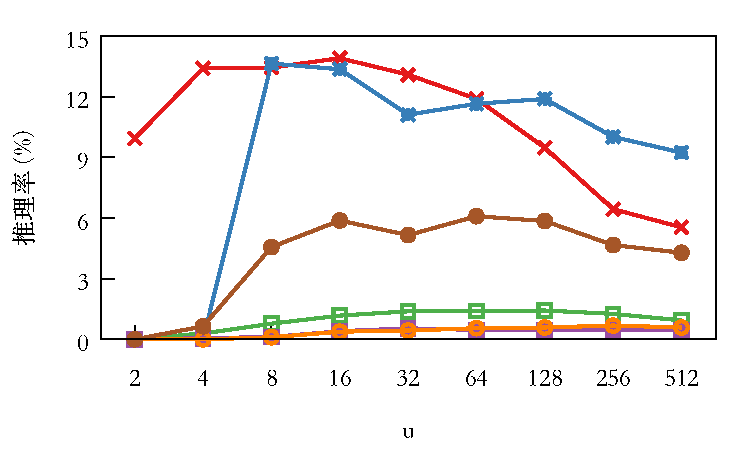
\includegraphics[width=\linewidth]{dis-impact-u-rate.pdf} &
        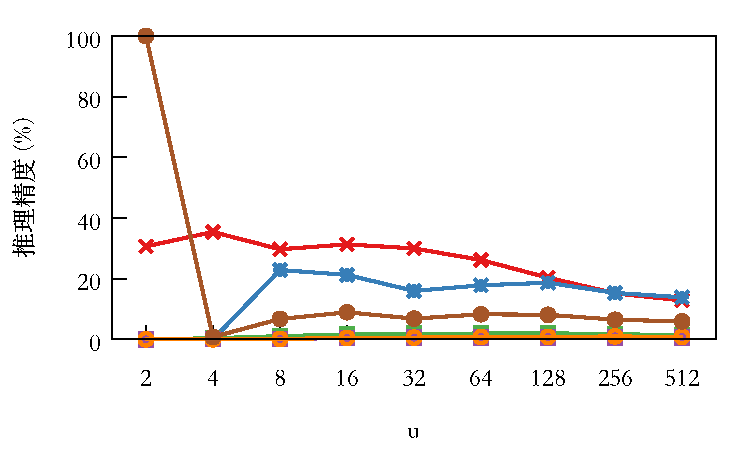
\includegraphics[width=\linewidth]{dis-impact-u-accuracy.pdf}\\
    \end{tabular}
    \caption{基于分布的攻击实验1:参数$u$的变化对推理结果的影响($r = 0$;$t \rightarrow \infty$)}
    \label{fig:distribution-impact-u}
\end{figure}

图\ref{fig:distribution-impact-u}显示了将参数$u$从2变为512时对推理率和推理精度带来的影响。对于推理率的结果,本实验的观察结果与已有的工作\citing{li2017information}相同。推理率首先随着$u$的增大而提高,这是因为频率分析攻击可以推理出更多的密文数据块-明文数据块对。推理率在达到最大值之后(例如,User004为13.9\%,User007为13.6\%,User012为1.4\%,User013为0.5\%,User015为0.7\%,User028为6.1\%)开始下降。其原因在于频率分析引入了大量的误报,这些误报会继续影响基于分布的攻击对每个数据块相邻邻居的推理。同时,部分特殊情况下的推理率约为0.0001\%,这意味着攻击只能推理出几个密文数据块-明文数据块对。

已有的工作\citing{li2017information}不提供基于数据块局部性的攻击的推理精度信息,因此本文提出的两种推理攻击方法的实验的推理精度的部分不与其进行对比。实验中观察到除User028的数据在$u=2$的条件下没有引入任何误报外,针对所有用户备份数据的推理精度都处于相当低的水平(小于40\%)。随着$u$的增大,推理精度会略有下降。例如,当$u$从2增加到512时,User004的推理精度从30.7\%下降到12.8\%。
    
\textbf{结论(1):}相对较大的$u$提高了推理率,但降低了推理精度(即,引入了更多的误报)


\subsubsection{参数$r$的影响}

然后,通过$u$变化的影响分析,本文选择增加推理的密文数据块-明文数据块对的覆盖范围,同时使用$r$和$t$来过滤可能的误报。因此,本文将User004,User013和User015的$u$设置为128,User007,User012和User028的设置分别为256,以评估$r$和$t$变化的影响。 

\begin{figure}[!htbp]
    \centering
    \begin{tabular}{p{.48\linewidth}p{.48\linewidth}}
        \multicolumn{2}{c}{
\includegraphics[width=.7\textwidth]{legend-fsl-line.pdf}}  \\
        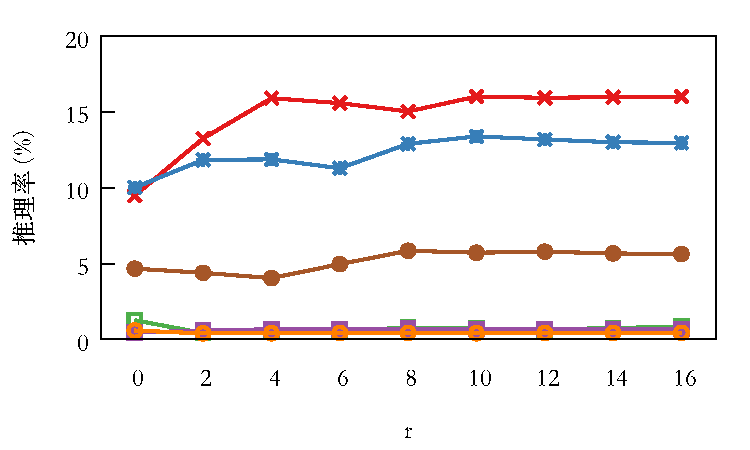
\includegraphics[width=\linewidth]{dis-impact-r-rate.pdf} &
        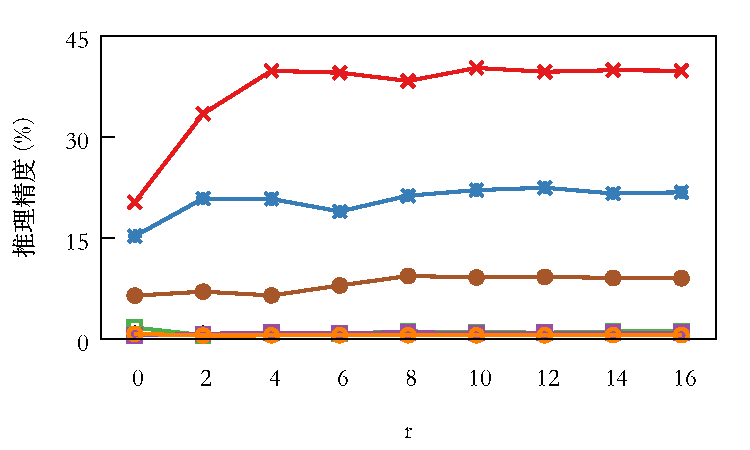
\includegraphics[width=\linewidth]{dis-impact-r-accuracy.pdf}\\
    \end{tabular}
    \caption{基于分布的攻击实验1:参数$r$的变化对推理结果的影响(User004、User013和User015中$u = 128$,User007、User012和User028中$u = 256$;$t \rightarrow \infty$)}
    \label{fig:distribution-impact-r}
\end{figure}

本实验中首先令$t\rightarrow \infty$,然后评估$r$变化带来的影响。图\ref{fig:distribution-impact-r}展示了参数$r$变化的实验结果。 实验观察到大多数用户的推理率随着$r$而增加。例如,当将$r$从0变为16时,User004推理率从9.5\%增加到16.0\%,User007从10.0\%增加到13.0\%,User013从0.5\%增加到0.7\%,User028从4.7\%增加到5.6\%。发生这种现象的原因是基于分布的攻击减少了直接频率排序的干扰,并推理出更多正确的密文数据块-明文数据块对。另一方面,对于User012和User015,推理率分别从1.3\%降至0.8\%,从0.6\%降至0.4\%。原因是随着检查的扩大,可能引入更多的误报。同时,所有用户的推理精度均处于低水平(小于45%),并且具有与其相应的推理率类似的变化趋势。


\textbf{结论(2):}较大的$r$提供了识别正确的密文数据块-明文数据块对的更多机会,但也增加了发生误报的概率。
\subsubsection{参数$t$的影响}

\begin{figure}[!ht]
    \centering
    \begin{tabular}{p{.48\linewidth}p{.48\linewidth}}
        \multicolumn{2}{c}{
\includegraphics[width=.7\textwidth]{legend-fsl-line.pdf}}  \\
        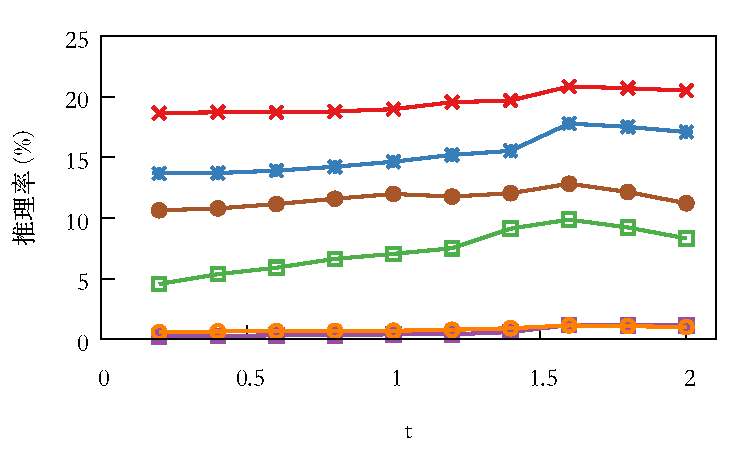
\includegraphics[width=\linewidth]{dis-impact-t-rate.pdf} &
        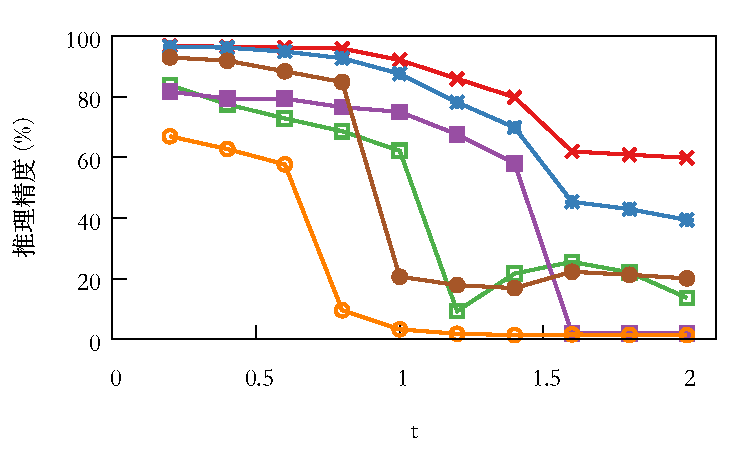
\includegraphics[width=\linewidth]{dis-impact-t-accuracy.pdf}\\
    \end{tabular}
    \caption{基于分布的攻击实验1:参数$t$的变化对推理结果的影响(User004、User013和User015中$u = 128$,User007、User012和User028中$u = 256$;$r = 10$)}
    \label{fig:distribution-impact-t}
\end{figure}

最后,设定$r=10$来评估参数$t$变化的影响。 图\ref{fig:distribution-impact-t}展示了参数$t$变化的实验结果果。当$t$很小(例如,小于0.5)时,实验观察到攻击误判并过滤了大量的密文数据块-明文数据块对,即使它们是正确的(即,引入了降低推理率的假阳性结果)。随着$t$的增加,假阳性的结果数量减少。当$t= 1.5$时,对于User004,User007,User012,User013,User015和User028,推理率分别达到最大值21.2\%,18.2\%,10.4\%,1.2\%,1.2\%和13.5\%。 当$t$进一步增大到2时,相应的推理率分别降至20.5\%,17.1\%,8.3\%,1.2\%,1.0\%和11.2\%。其原因是如果$t$过大,攻击就无法有效地过滤误报。因此,所有用户数据的推理精度都会随着$t$的增大而下降。

\textbf{结论(3):}较小的$t$过滤了大部分频率分析带来的误报,但它引入了更多的假阳性结果,导致了推理率的下降。

\subsection{实验2(与已有工作的对比)}
\label{sec:exp2}
本文将基于分布的攻击的有效性与基于数据块局部性的攻击的有效性进行比较\citing{li2017information}。除了使用实验1(参见\ref{sec:exp1})中采用的FSL数据集之外,本文还加入MS数据集(参见\ref{sec:ubc-ms})用于进行跨数据集的验证与评估。在MS数据集中,对于每个系统类别,一次选择两个快照,使用其中一个来推理另一个,以此评估平均的推理率和推理精度。

本文考虑采用以下攻击实例来进行比较。

\begin{itemize}[leftmargin=*]
\item \textbf{$\tt Baseline$:}

实验根据已有工作\citing{li2017information}中建议的参数配置实现基于数据块局部性的攻击。具体来说,它在频率分析的第一次调用中推理出5个出现频率最高的的密文数据块-明文数据块对(即,初始化一组用于迭代的密文数据块-明文数据块对),并且在每次后续调用中根据已有数据块对的邻居推理30个新的数据块对(即,迭代地推理密文数据块-明文数据块对)。

\item \textbf{$\tt Distribution$和$\tt Distribution^S$:} 

考虑两个基于分布的攻击的攻击实例,分别由$\tt Distribution$和$\tt Distribution^S$表示,它们分别使用和不使用大小信息作为辅助信息(即上标$\tt S$表示攻击实例使用大小信息进行操作)。实验在与${\tt Baseline}$相同参数的条件下配置$\tt Distribution^S$和${\tt Distribution}$。 此外,实验通过以下方式在$\tt Distribution^S$和${\tt Distribution}$中选择参数$r$和$t$的取值:对于FSL数据集,我们为所有用户设定$r = 10$,并分别为User004、User007、User012、User013、User015和User028设置参数$t$ = 1.5、1.2、1、1、0.7和0.9;对于MS数据集,实验继续为所有类别设置参数$r = 10$,为Win7和Serv-08设置参数$t = 2$,为Vista-U、Serv-03和Vista-B设置参数$t = 1.6$。以上数据是通过按照实验1(参见\ref{sec:exp1})的方法对数据集的最佳配置的测试得出的。 
\item \textbf{$\tt Distribution$-$\tt o$和$\tt Distribution^S$-$\tt o$:}

实验考虑另外两个基于分布的攻击的实例,用$\tt Distribution$-$\tt o$和$\tt Distribution^S$-$\tt o$表示,对于$r$和$t$应用与$\tt Distribution$和$\tt Distribution^S$相同的配置,但进一步使用更大的参数$u$增加推理的密文数据块-明文数据块对的覆盖范围。具体来说,实验通过以下方式在$\tt Distribution$-$\tt o$和$\tt Distribution^S$-$\tt o$中配置参数$u$:对于FSL数据集,参数$u$的选择与实验1(参见\ref{sec:exp1})相同;对于MS数据集,实验为Win7数据设置$u = 128$,为Serv-03、Serv-08、Vista-B和Vista-U设置$u  = 30$。 
\end{itemize}

\begin{figure*}[!htbp]
    \centering
    \begin{tabular}{c}
        
\includegraphics[width=.7\textwidth]{pic/legend-fsl-bar.pdf}\\
        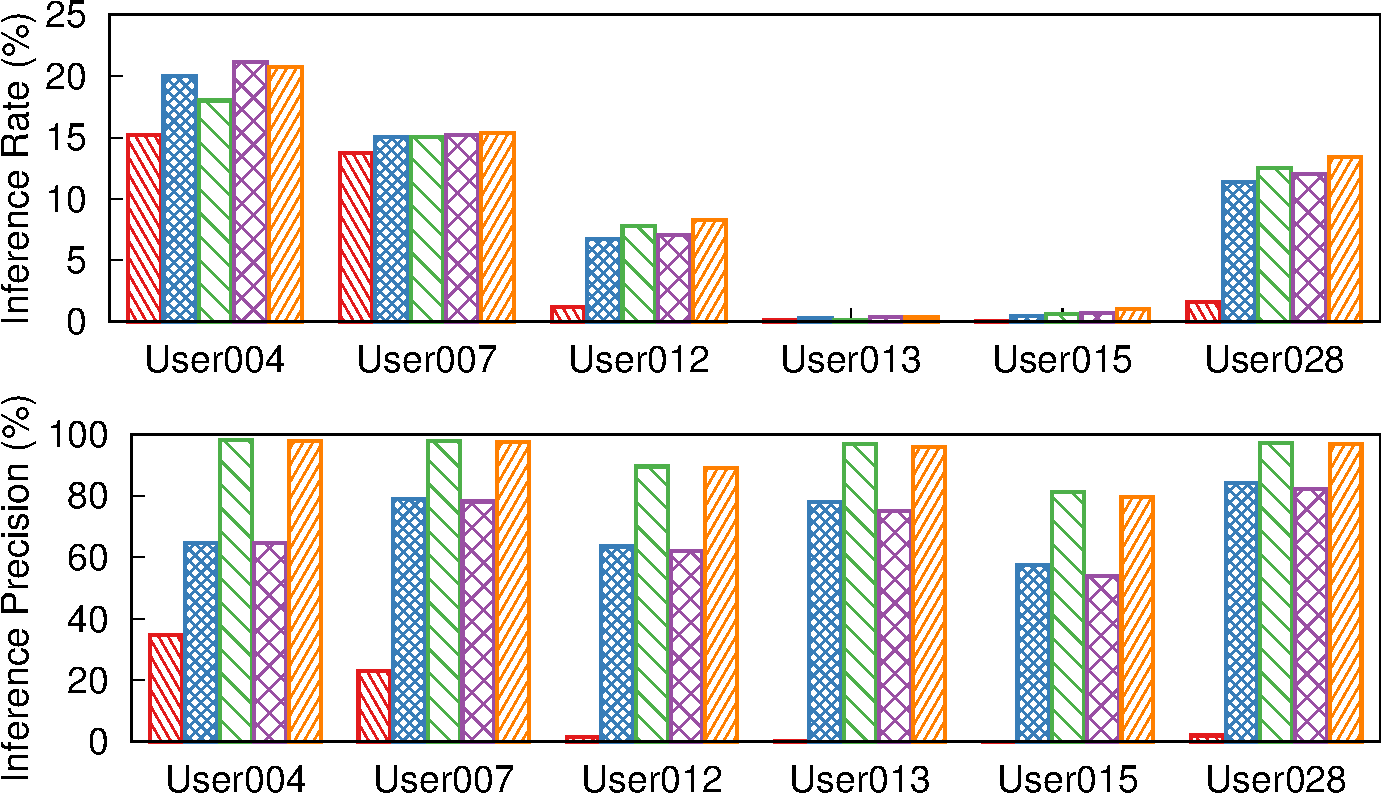
\includegraphics[width=.7\textwidth]{pic/distribution-comparison-fsl.pdf} 
    \end{tabular}
    \caption{基于分布的攻击实验2(与已有工作的对比):比较基于分布的攻击和基于数据块局部性的攻击的有效性(FSL数据集)。}
    \label{fig:distribution-comparison-fsl}
\end{figure*}

图\ref{fig:distribution-comparison-fsl}给出了基于FSL数据集的上述5种实例的比较结果。实验观察到,在几乎所有情况下,基于分布的攻击的不同实例都优于基于数据块局部性的攻击。例如,对于User028,基于分布的攻击的最低推理率是11.4\%,推理精度为84.1\%($\tt Distribution$);此时$\tt Baseline$相应的推理率仅为1.2\%,推理精度仅为1.7\%。这意味着在这种情况下,基于分布的攻击可以将假阳性的数量减少82.4\%。

\textbf{结论(4):}基于分布的攻击显着提高了推理精度,同时实现了比基于数据块局部性的攻击更高的推理率。 

$\tt Distribution^S$和$\tt Distribution^S$-$\tt o$相较于$\tt Distribution$和$\tt Distribution$-$\tt o$拥有更高的推理精度,这因为它们进一步通过数据块大小信息过滤了误报。例如,对于User004,$\tt Distribution^S$和$\tt Distribution^S$-$\tt o$相较于$\tt Distribution$和$\tt Distribution$-$\tt o$将误报分别从35.2\%减少到1.7\%,从35.3\%减少到2.2\%。然而,在同样的情况下,实验观察到$\tt Distribution$ and $\tt Distribution$-$\tt o$的推理率分别为20.0\%和21.2\%,相较于$\tt Distribution^S$和$\tt Distribution^S$-$\tt o$分别高出2.0\%和0.4\%。其原因是$\tt Distribution$和$\tt Distribution$-$\tt o$推理出了来自不正确的密文数据块-明文数据块对的邻居中的少量正确结果。换句话说,虽然$(C, M)$是不正确的密文数据块-明文数据块对,但$C$的邻居可能以很小的概率对应于$M$的邻居。即使在这种情况下,所有基于分布的攻击实例都比基于数据块局部性的攻击实例效果更佳。具体来说,$\tt Baseline$的推理率仅为15.2\%,比基于分布的攻击的最佳情况低6.0\%,最差情况低2.8\%。  

\textbf{结论(5):}过滤不正确的推理结果可以提高推理精度,但会降低推理的密文数据块-明文数据块对的覆盖范围,并可能降低推理率。

我们进一步观察到,虽然$\tt Distribution$-$\tt o$和$\tt Distribution^S$-$\tt o$构建在更大的参数$u$上,但它们的推理率仅略高于$\tt Distribution$和$\tt Distribution^S$(分别高为0.4\%和0.9\%)。 原因是基于分布的攻击仅通过已推理出数据块对的邻居进行迭代推理。参数$u$的进一步增大只会在结果中添加少量新的正确密文数据块-明文数据块对。

\begin{figure*}[t]
    \centering
    \begin{tabular}{c}
        
\includegraphics[width=.7\textwidth]{pic/legend-fsl-bar.pdf}\\
        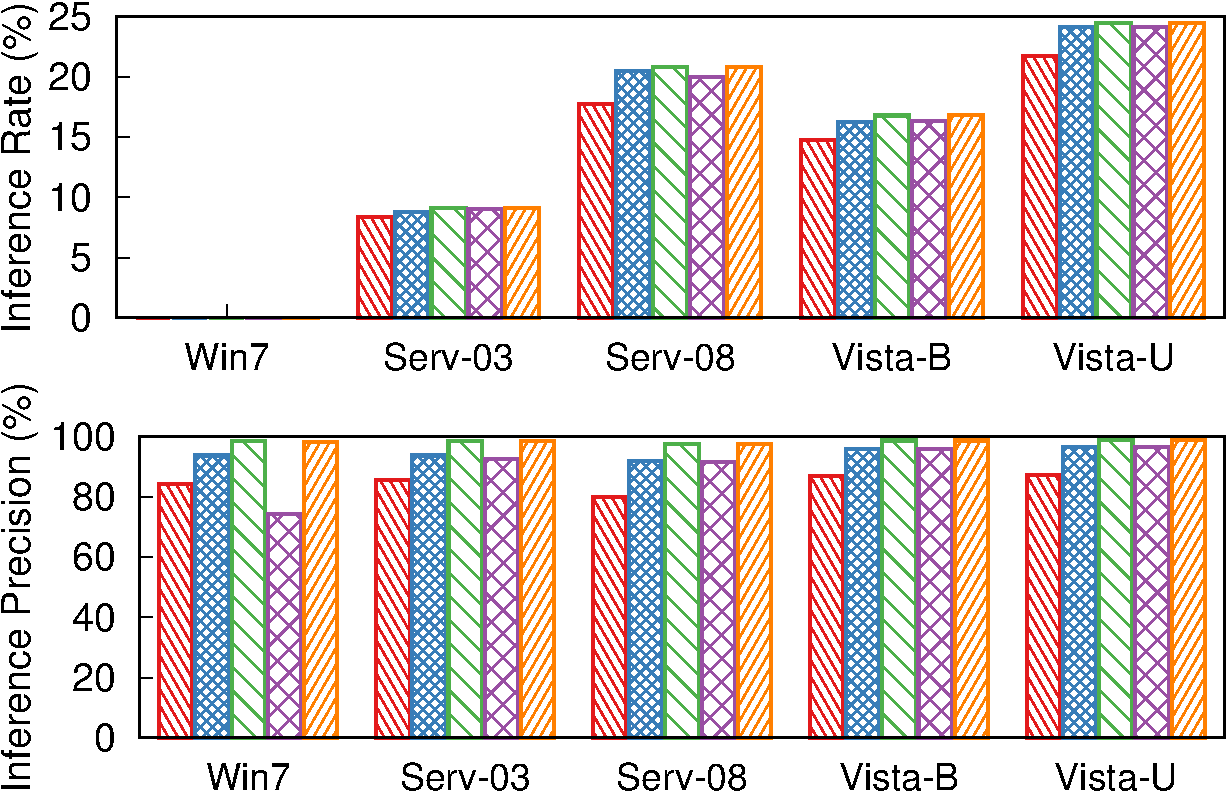
\includegraphics[width=.7\textwidth]{pic/distribution-comparison-ms.pdf}\\
    \end{tabular}
    \caption{基于分布的攻击实验2(与已有工作的对比):比较基于分布的攻击和基于数据块局部性的攻击的有效性(MS数据集)。}
    \label{fig:distribution-comparison-ms}
\end{figure*}


图\ref{fig:distribution-comparison-ms}给出了基于MS数据集的上述5种实例的比较结果。基于数据块局部性的攻击和基于分布的攻击在大多数MS数据集的类别(Win7除外)中具有高推理率和精度。可能的原因是MS数据集中的快照高度相关(例如,数据块总数的方差很小,如表\ref{tab:MS-dataset}所示)。实验观察到基于分布的攻击仍然优于基于数据块局部性的攻击。例如,在Vista-U中,基于分布的攻击的所有推理的推理率和推理精度分别高于24.1\%和96.4\%,而$\tt Baseline$的推理率和分辨率分别为21.7\%和87.1\%。

实验中对于数据集中Win7类别,基于分布的攻击和基于数据块局部性的攻击的推理率都很低(小于0.01%)。其原因是Win7包含大量具有唯一性的数据块(大约超过98.8\%,如表\ref{tab:MS-dataset}所示),导致了攻击效果表现不佳。

\subsection{实验3(攻击效果)} 
\label{sec:exp3}
实验考虑长期备份模式,并使用FSL数据集检查基于分布的攻击的有效性。具体来说,实验选择每个用户的第$i$个FSL每周备份作为辅助信息,以推理相应的第$(i+w)$个FSL每周备份中的原始明文。显然,$w$越小,辅助信息和目标备份之间的相关性就越高。与实验2(参见\ref{sec:exp2})配置两个基于分布的攻击实例$\tt Distribution$-$\tt o$和$\tt Distribution^S$-$\tt o$,并评估它们的推理率和推理精度(针对每个用户的所有可用的$i$)。

\begin{figure*}[!htbp]
    \centering
    \centering
    \begin{tabular}{c}
        
\includegraphics[width=.35\textwidth]{legend-effectiveness.pdf}\\
        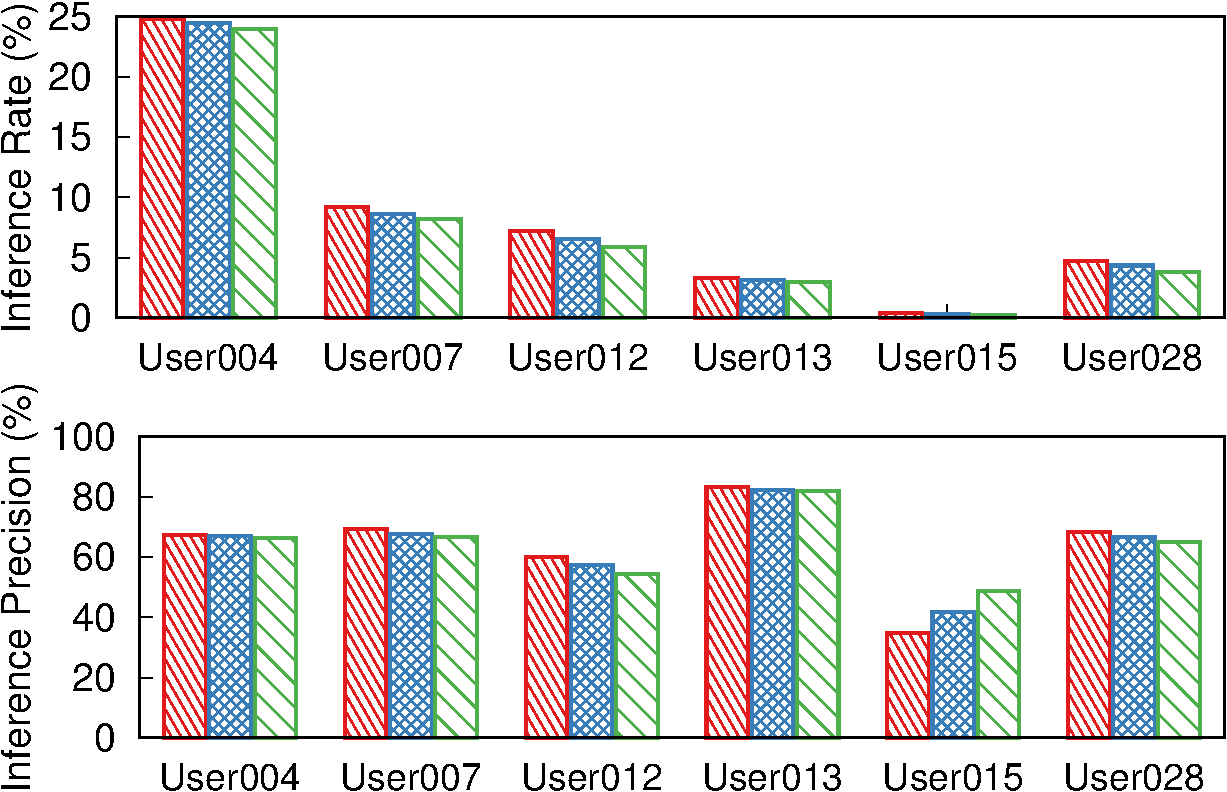
\includegraphics[width=.7\textwidth]{distribution-effectiveness-wo-size.pdf}
    \end{tabular}
	\caption{实验3(攻击效果):没有大小信息辅助的基于分布的攻击在FSL数据集中的有效性。}
	\label{fig:experiment-distribution-effectiveness-wo}
\end{figure*}

图\ref{fig:experiment-distribution-effectiveness-wo}给出了$\tt Distribution$-$\tt o$的实验结果。基于分布的攻击在用户之间具有不同的推理率和推理精度。例如,在类似User004这样的有利情况下,它实现了推理率24.8\%、推理精度67.3\%($w = 1$);推理率24.5\%、推理精度67.0\%($w = 2$);推理率24.0\%、推理精度66.5\%($w = 3$)。在类似User015这样的非有利情况下,基于分布的攻击的推理率仅有0.3\%。可能的原因是User015的备份数据具有较低的数据块局部性。

此外,实验观察到辅助信息的相关性(即$w$)对基于分布的攻击的有效性影响较低。例如,当$w$从1增加到3时,它仅导致推理率(下降小于1.4\%)和精度(下降小于5.6\%)的有限下降。其原因是基于分布的攻击解决了频率排名中的干扰并保留了攻击的有效性。

\textbf{结论(6):}基于分布的攻击可以在存在松散相关的辅助信息的帮助下有效控制攻击有效性的下降程度。

\begin{figure*}[!htbp]
    \centering
    \centering
    \begin{tabular}{c}
        
\includegraphics[width=.35\textwidth]{pic/legend-effectiveness.pdf}\\
        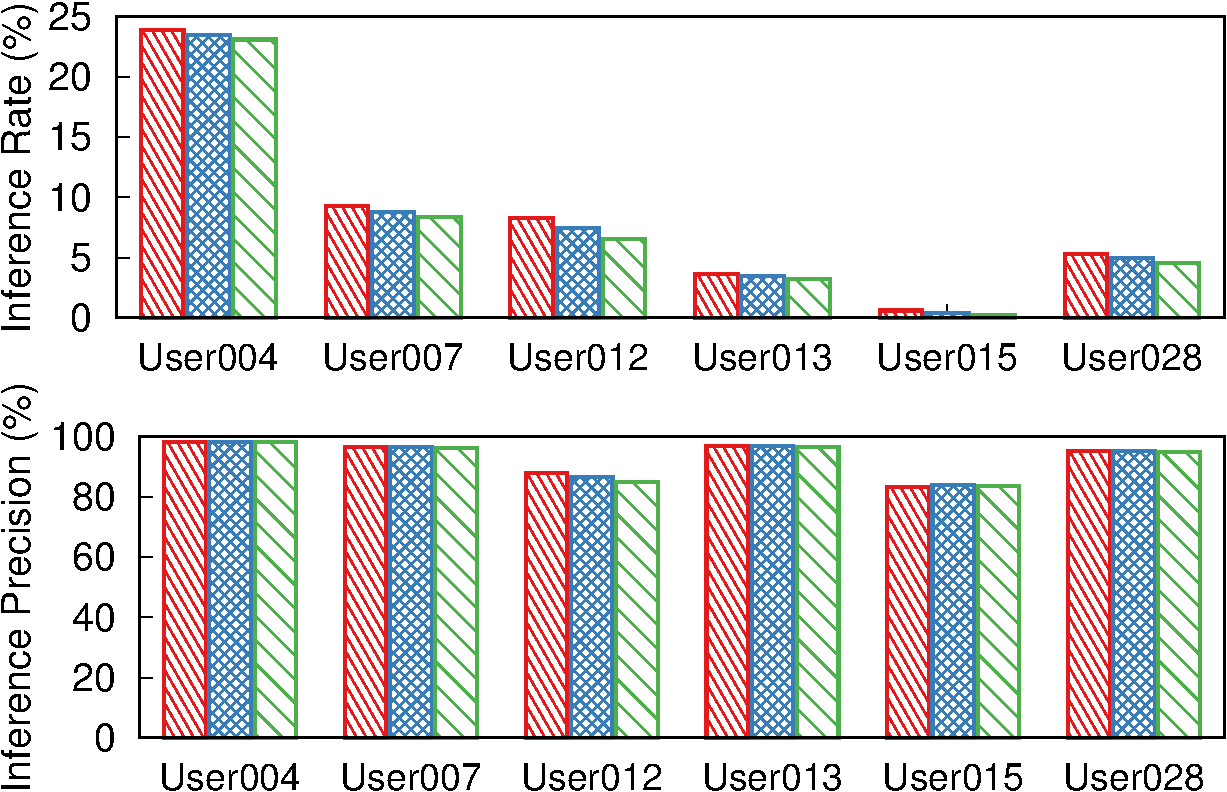
\includegraphics[width=.7\textwidth]{pic/distribution-effectiveness-w-size.pdf}
    \end{tabular}
	\caption{实验3(攻击效果):有大小信息辅助的基于分布的攻击在FSL数据集中的有效性。}
	\label{fig:experiment-distribution-effectiveness-w}
\end{figure*}

图\ref{fig:experiment-distribution-effectiveness-w}给出了$\tt Distribution^S$-$\tt o$的实验结果。实验观察到它具有与$\tt Distribution$-$\tt o$相似的推理率,同时拥有更高的推理精度。例如,对于所有用户的平均推理精度分别为93.1\%($w = 1$)、92.8\%($w = 2$)和92.4\%($w = 3$)。         

\section{基于聚类的攻击的实验结果}
\label{sec:experiment-clustering}

\subsection{实验4(参数的影响)} 
\label{sec:exp4}
实验首先评估参数$k$的影响,该参数定义了凝聚法层次聚类中组合两个最近聚类的距离上限。本实验使用FSL和VM数据集来研究$k$如何影响攻击中的基础聚类方案。具体来说,分别对每个选出的FSL和VM用户数据的最后一次备份应用分段方法,并生成固定大小为4MB的数据段。

聚类方案旨在将类似的密文数据段聚合到同一个聚类中,这一过程不会损害每个密文数据段中的数据块的机密性。本文使用聚类接近度量化其影响,将聚类的结果与实际分类方法的结果进行比较(实际分类方法通过最小数据块哈希直接对分段进行分类)。假设我们分别通过实际分类方法生成$m$个数据段的集合,并且通过聚类方案生成$\widetilde{m}$个数据段的集合。通过$\frac{{\sf abs}(m-\widetilde{m})}{m}$(其中${\sf abs}(m-\widetilde{m})$返回$m-\widetilde{m}$的绝对值)衡量聚类形成的集合与实际分类形成的集合的相似程度。记集合所有数据段都相同(具有相同的最小数据块哈希)的聚类的数量为$\hat{m}$。此外,实验还考虑了聚类正确性,通过$\frac{\hat{m}}{\widetilde{m}}$进行评估,它量化了对相似数据段的聚类方案的精确程度。

\begin{figure}[!htbp]
    \centering
    \begin{tabular}{p{.48\linewidth}p{.48\linewidth}}
        \multicolumn{2}{c}{
\includegraphics[width=.5\textwidth]{clu-fsl-bar.pdf}}  \\
        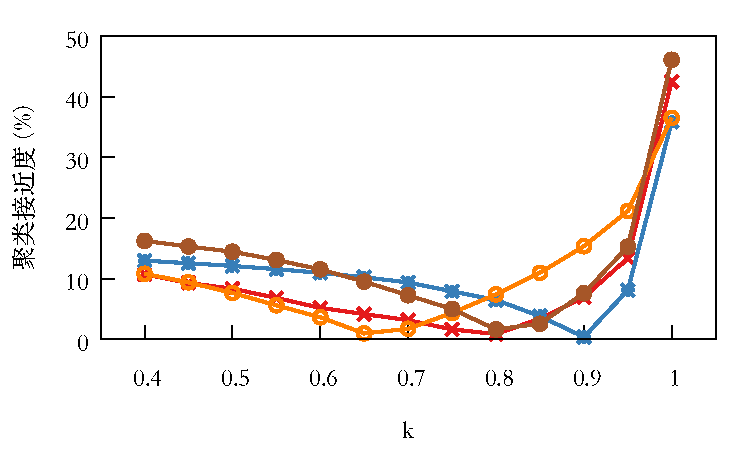
\includegraphics[width=\linewidth]{clu-impact-d-fsl-clo.pdf} &
        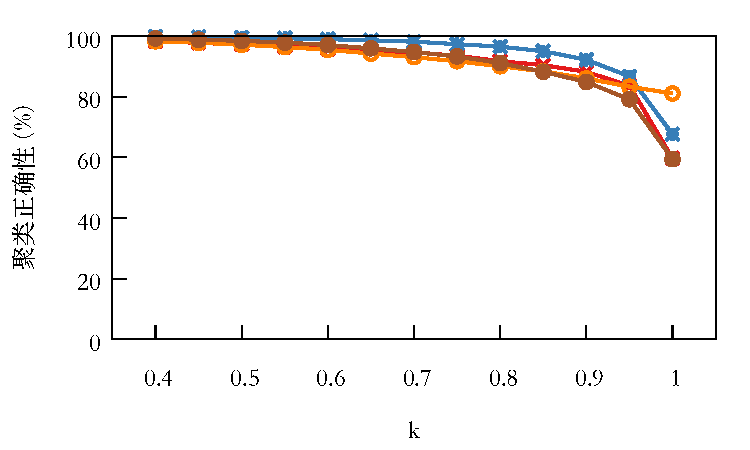
\includegraphics[width=\linewidth]{clu-impact-d-fsl-cro.pdf}\\
    \end{tabular}
    \caption{实验4(参数的影响):FSL数据集中参数$k$对基于聚类的攻击的影响(聚类接近度越小越好;聚类正确性越大越好)。}
    \label{fig:cluster-impact-d-fsl}
\end{figure}

图\ref{fig:cluster-impact-d-fsl}给出了针对FSL数据集的实验结果,其中考虑了四个FSL用户的数据(User004,User007,User015和User028)以节省评估时间。 聚类接近度首先随$k$的增加而增加,这是因为聚类的数量(即$\widetilde{m}$)减少并接近$m$。当$k$进一步增加时,聚类数量会从$m$开始下降,并导致聚类间接近度的增加。此外,实验观察到聚类正确性随$k$的增大逐渐减小,这是因为一些非相似的数据段(即,它们的最小块散列不同)被聚合到同一聚类中。这两个结果都表明攻击者可以通过配置一个合适的$k$来平衡聚类的接近程度和正确性的关系。 例如,当我们为User015设置$k = 0.65$时,相应的聚类接近度和正确性分别为1.0\%和94.2\%。这意味着聚类方案的结果高度接近实际分类的结果。
            
\textbf{结论(7):}通过为聚类方法配置适当的参数$k$,攻击可以在未知数据段的最小数据块哈希的前提下得到近似的分类效果。

\begin{figure}[!htbp]
    \centering
    \begin{tabular}{p{.48\linewidth}p{.48\linewidth}}
        \multicolumn{2}{c}{
\includegraphics[width=.7\textwidth]{clu-vm-bar.pdf}}  \\
        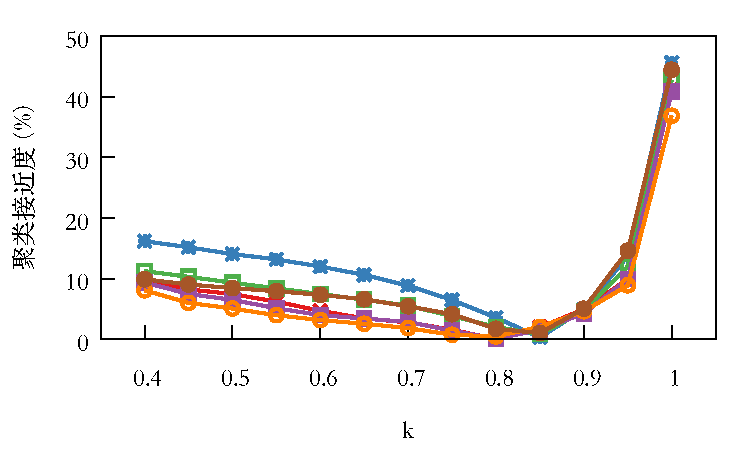
\includegraphics[width=\linewidth]{clu-impact-d-vm-clo.pdf} &
        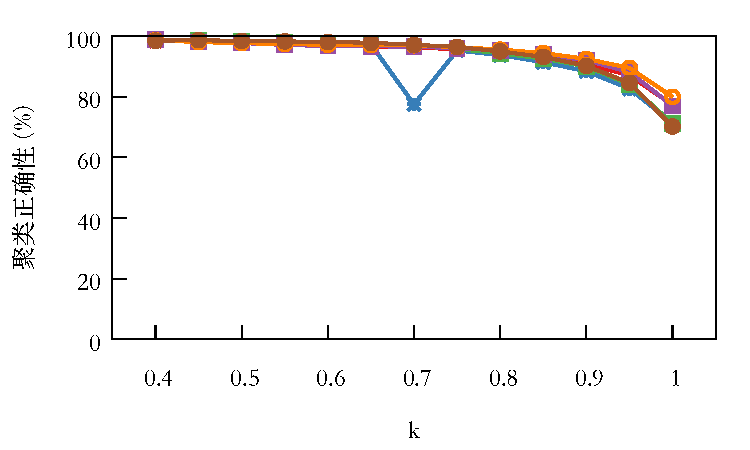
\includegraphics[width=\linewidth]{clu-impact-d-vm-cro.pdf}\\
    \end{tabular}
    \caption{实验4(参数的影响):VM数据集中参数$k$对基于聚类的攻击的影响(聚类接近度越小越好;聚类正确性越大越好)。}
    \label{fig:cluster-impact-d-vm}
\end{figure}

图\ref{fig:cluster-impact-d-vm}给出了针对VM数据集的实验结果。实验观察到所有VM数据集中的用户数据的聚类接近度和正确性与FSL数据集中的用户数据具有相似的趋势。当配置参数$k = 0.8$时,所有VM数据集中的用户数据的平均聚类接近度为3.0\%,相应的聚类正确性高达93.1\%。

\subsection{实验5(攻击效果)} 
\label{sec:exp5}
本实验研究基于聚类的攻击的有效性。由于固定大小的数据段的边界移位问题,它对FSL数据集的有效性很低(在本实验的测试中大约仅有1\%的推理率)。因此,本实验使用VM数据集来评估其有效性。在基于聚类的攻击中,为聚类方法设置参数$ k  = 0.8$,并配置$(u, r, t) = (5000, 100, 0.5)$用于将密文聚类与相应的明文聚类相关联。

在本实验的基准测试中,实验发现基于聚类的攻击中的数据块级推理仅正确地推理出数千个数据块(推理率过低,小于0.01\%)。因此,本文重点研究数据段级的推理,它给出了基于聚类的攻击的有效性的下限。为了与数据块级推理效果的测量保持一致,实验基于每个正确推理的数据段中的唯一性的数据块个数来计算推理率和推理精度。 

\begin{figure}[!htbp]
    \centering
    \begin{tabular}{p{.48\linewidth}p{.48\linewidth}}
        \multicolumn{2}{c}{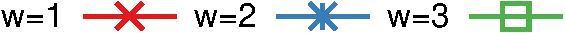
\includegraphics[width=.35\textwidth]{clu-effect-bar.pdf}}  \\
        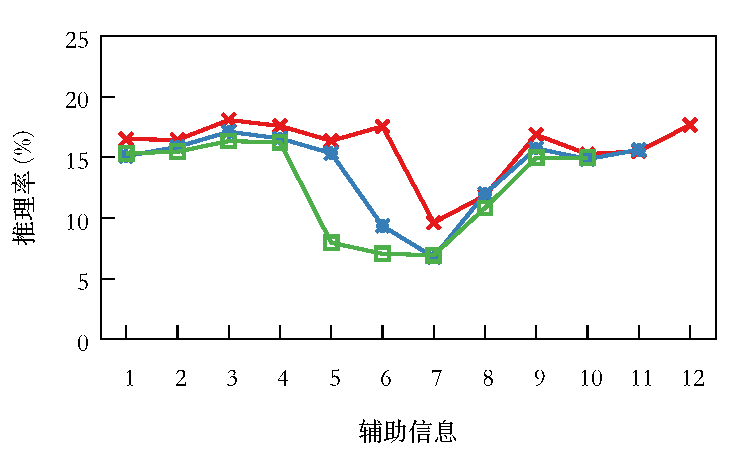
\includegraphics[width=\linewidth]{clu-effect-rate.pdf} &
        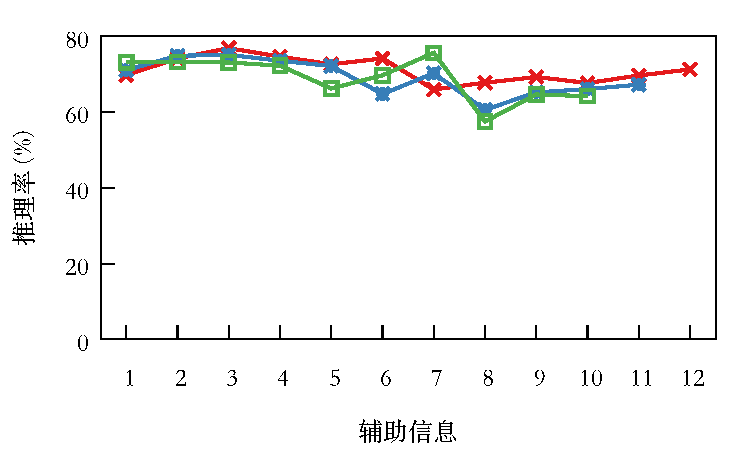
\includegraphics[width=\linewidth]{clu-effect-pre.pdf}\\
    \end{tabular}
    \caption{实验5(攻击有效性):VM数据集中基于聚类的攻击的有效性。}
    \label{fig:cluster-effect}
\end{figure}

本实验采取与实验3(参见\ref{sec:exp3})相同的评估方法,实验结果如图\ref{fig:cluster-effect}所示。具体来说,X轴描述了VM备份数据集中的第$i$(其中1 $ \leq i \leq $ 12)个备份用作攻击的辅助信息,而y轴表示该辅助信息对VM数据集中第$(i + w)$(其中$w = 1,2,3$)个备份的平均推理效果。实验观察到推理率和推理精度都有显著波动。例如,当使用第3个备份作为辅助信息时,攻击的推理率为18.1\%,推理精度为76.8\%($w = 1$);推理率为17.1\%,推理精度为75.0\%($w = 2$);推理率为16.3\%,推理精度为73.0\%($w = 3$)。但当使用第7个备份作为辅助信息时,相应的推理率和推理精度分别下降到9.6\%和65.9\%;6.8\%和71.2\%;以及6.9\%和75.6\%。原因是VM数据集中的备份在第7周之后有大量更新,显著减少了相邻备份间的相关性。平均而言,对于$w = 1,2,3$时,基于聚类的攻击推理出15.8\%,14.0\%和12.6\%密文数据块-明文数据块对,对应的推理精度为71.1\%,69.1\%,和68.9\%。

\section{攻击对安全影响的结果}
\label{sec:case}

到目前为止,本文通过量化正确推理的密文数据块-明文数据块对来检查推理攻击的有效性。然而,这些结果所带来的安全隐患以及频率分析攻击如何带来实际损害仍然是一个悬而未决的问题。在下面的实验中,本文根据原始推理率评估攻击的安全隐患,原始推理率定义为受正确推理的数据块影响的原始数据块的百分比。

\subsection{实验6(安全隐患分析)}
\label{sec:exp6}
实验首先考虑基于分布的攻击,并针对不同类型的文件评估其原始推理率。这一部分使用FSL数据集来进行评估,因为只有FSL数据集包含数据块所属的文件的文件元数据(包含文件的扩展名)。具体来说,本实验关注具有特定扩展名的五种类型的文件(参见表\ref{tab:exp-fsl-file-dis}):office文件,图片文件,程序源代码文件,数据库文件和磁盘映像文件。这些文件占FSL数据集原始内容的60\%以上。

\begin{table}[!htbp]
\small
\caption{实验6(安全隐患分析):基于分布的攻击}
\label{tab:exp-fsl-file-dis}
\centering
\begin{tabular}{|c|c|c|c|c|c|}
\hline

    \multirow{2}{*}{\bf 文件类型} & \multirow{2}{*}{\bf 扩展名} & \multirow{2}{*}{\bf \centering 文件大小范围}  & \multicolumn{2}{c|}{\bf 原始推理率} \\ \cline{4-5} 
    & & &  $\sf Distribution$-$\sf o$ & $\sf Distribution^S$-$\sf o$ \\ \hline
    Office文件 & doc(x), ppt(x), xls(x) & 10KB-1MB   & 4.9\% & 5.3\%\\
\hline
    图片文件 & jpg, png &10-100KB  & 7.7\% & 6.7\% \\
\hline
    程序源代码 & c, h, cpp, java, py & 10-20KB   & 17.1\% & 15.0\%\\
\hline
    数据库文件 & db, po & 20-700KB   & 2.6\% & 2.4\%\\
\hline
    磁盘映像文件 & vmdk, img & 200MB-1GB  & 15.8\% & 16.7\%\\
\hline
\end{tabular}
\end{table}


这一部分应用实验2(参见\ref{sec:exp2})提出的方法的方法,用$\sf Distribution^S$-$\sf o$和$\sf Distribution$-$\sf o$来评估机遇分布的攻击的原始推理率。表\ref{tab:exp-fsl-file-dis}给出了实验结果。两种攻击实例针对磁盘映像文件都具有较高的原始推理率(例如,$\sf Distribution$-$\sf o$为15.8\%,$\sf Distribution^S$-$\sf o$为16.7\%),这因为每个磁盘文件中包含大量很少进行更新的数据块,这些数据块在同一文件中具有很强的数据块局部性。有趣的是,实验观察到程序源代码文件中,尽管每个文件都很小,但基于分布的攻击也具有很高的原始推理率(例如,$\sf Distribution$-$\sf o$为17.1\%,$\sf Distribution^S$-$\sf o$为15.0\%)。其原因是程序源代码文件通常一起存储在文件系统中(例如,属于同一项目的源文件位于相同的目录中)并形成大范围的相关数据块,在文件之间具有很强的数据块局部性。对于小型或分散的文件(例如,Office文件,图片文件和数据库文件),基于分布的攻击的原始推理率相对较低。

\textbf{结论(8):}基于分布的攻击的有效性取决于目标文件的更新频率,文件大小和存储结构。

这一部分使用VM数据集评估基于聚类的攻击带来的安全隐患。具体来说,本实验使用每个VM用户数据的第11个备份来推理该用户相应的第13个中的原始数据内容。由于VM数据集不包含任何元数据,因此本实验根据每个VM快照中的所有数据块计算原始推理率。请注意,本实验在原始推理率的计数中过滤所有全零数据块,因为它们在VM磁盘映像中占有很大比例\citing{jin2009effectiveness},且会对评估的结果产生误导(导致原始推理率结果虚假偏高)。

\begin{table}[!htbp]
\small
    \caption{实验6(安全隐患分析):基于聚类的攻击}
    \centering
    \begin{tabular}{|c|c|c|c|}
    \hline
        {\bf 用户ID} & {\bf 原始推理率} & {\bf 用户ID} & {\bf 原始推理率}\\
    \hline
        1 & 13.2\% & 2 & 22.4\% \\ 
    \hline
        3 & 25.7\% & 4 & 28.4\% \\ 
    \hline
        5 & 18.5\% & 6 & 30.8\% \\ 
    \hline
    \end{tabular}
\label{tab:exp-vm-user-cluster}

\end{table}

这一部分使用与实验5(参见\ref{sec:exp5})相同的配置,并在通过数据段级推理来评估原始推理率。 表\ref{tab:exp-vm-user-cluster}给出了不同用户数据的原始推理率结果。实验观察到基于聚类的攻击对VM数据集实现了很高的安全威胁。例如,它可以推理出User6的VM备份中高达30.8\%的原始内容。所有用户的平均原始推理率高达23.2\%。

\textbf{结论(9):}基于聚类的攻击严重威胁到VM磁盘映像的机密性。
\section{本章小结}
本章通过6个实验对基于分布的攻击和基于聚类的攻击的相关参数的影响、攻击的有效性以及两种攻击手段对真实世界数据集的安全威胁进行了验证与分析,提出了9个根据实验观察得出的结论,证明了两种攻击手段的作用和价值。


\chapter{应对频率分析攻击的对策讨论}
\label{sec:Countermeasure}

在本章中,将讨论应对本文攻击方案使用的三种泄漏的对策及其优缺点。但在三中泄漏中,单纯的防范数据块大小信息泄漏并不足以使本文提出的攻击手段失效(大小信息的利用只是攻击用于进一步提高推理攻击准确性的可选条件)。

\section{防止频率泄漏}

MinHash加密\citing{qin2017design,li2017information}使用从一组相邻数据块上的最小块哈希导出的密钥加密该组内每个明文数据块,因此可能将相同的明文数据块加密映射到不同的密文数据块。防御频率信息泄漏的基本原理是通过MinHash加密改变各个密文数据块的频率,并由此扰乱不同数据块的频率排名。

与此同时,MinHash加密还可以用于防止本文中的频率分析攻击。MinHash加密是非确定性的加密方法,使用该方法会改变数据块的频率分布,因此本文的的攻击目标是确定性加密(例如,MLE\citing{bellare2013message})。但MinHash加密因为打破了明文数据块-密文数据块之间的一一映射关系,所以在加密重复数据删除中导致了存储效率的下降(重复数据删除所能节省的存储空间变小)。此外,因为MinHash加密的随机性主要取决于目标工作负载中的最小块哈希,所以其不是一种扰乱数据块频率的主动对策,在不同的工作负载中能实现的扰乱效果具有较大的差异。         

最近的一项工作\citing{zuo2018mitigating}提出通过有计划的添加冗余(重复)的数据块来防止针对客户端加密重复数据删除的流量分析攻击。该方法\citing{zuo2018mitigating}在运作中会改变数据块的频率,因此可以用于防止频率分析攻击。与MinHash加密相比,该方法\citing{zuo2018mitigating}只是添加了重复的数据块,因此不会降低存储效率。但另一方面,它需要使用在特定的假设之下。首先它要求特定的数据块是重复的,其次它只适用于客户端重复数据删除。因此使用这种方法可能会引入额外的泄漏通道(参见\ref{sec:RelatedWork})。

现有工作提出了几个扩展的MLE实例基于强加密原语构建,以防止加密重复数据删除的频率泄漏,例如支持等式测试的随机加密\citing{abadi2013message},混合加密\citing{stanek2014secure},以及与完全同态加密的交互\citing{bellare2015interactive}。它们都提供了可证明的安全性,但它们如何在实践中实施和部署仍未有进一步的研究。

\section{防止顺序泄漏} 

一个简单的对策是干扰数据块在重复数据删除处理中顺序。例如,加密重复数据删除可以在加密之前对明文数据块流进行额外的顺序扰动添加处理,以隐藏每个明文数据块的真实逻辑顺序。这种方法可以有效的防止基于分布的频率分析攻击(参见\ref{sec:DistributionAttack}),因为攻击者无法正确识别到数据块邻居信息。但它对于基于聚类的频率分析攻击(参见\ref{sec:ClusteringAttack})并不是完全有效的。如果添加扰动仅在很小的范围内进行(例如,每个数据段中的明文数据块的顺序被添加扰动),则基于聚类的频率分析攻击方法仍然有效。

顺序扰乱策略的最大缺陷在于它破坏了数据块的局部性并且在大规模的重复数据删除中会导致性能的严重下降\citing{xia2011silo,zhu2008avoiding,lillibridge2009sparse}。

\section{防止大小泄漏}

正如已有的工作\citing{ritzdorf2016information}所建议的那样,加密重复数据删除可以在每个明文数据块种填充额外的数据来混淆这个明文数据块的实际大小。但是,这种填充方案的实现存在很大的难度,因为它需要在相同的明文数据块中添加相同的冗余数据;否则加密重复数据删除存储系统无法正常检测数据块是否重复。一种可能的解决方案建立在MLE\citing{keelveedhi2013dupless,bellare2013message}的范例之上,考虑将每个明文数据块的加密哈希作为计算种子,并使用它来生成可变大小的伪随机数据用于明文数据块的填充。与MLE一样,这种解决方案的代价是需要使用服务器辅助方法\citing{keelveedhi2013dupless}来抵御暴力攻击(参见\ref{sec:RelatedWork})。   


另一种思路是使用固定大小的数据块分块方法来取代可变大小的数据块分块方法。在这种情况下,由于所有的数据块都具有相同的大小,因此攻击者无法利用大小信息来区分它们。虽然固定大小的分块会受到边界偏移的影响,但它在VM磁盘映像这一特定数据类型中实现了与可变大小数据块分块方案几乎相同的重复数据删除存储空间节省效果\citing{jin2009effectiveness}。 因此,本文建议在某些特定的加密重复数据删除工作负载(例如,VM磁盘映像)中应用固定大小的数据块分块方法,以防止数据块大小信息泄漏。

\section{本章小结}

本章给出了应对三种类型泄漏带来的风险的方案,并比较了现有方案的优缺点。

\chapter{相关工作}
\label{sec:RelatedWork}

\section{MLE的应用}

回顾\ref{sec:background},MLE\citing{bellare2013message}正式确立了加密重复数据删除的加密方案基础。第一个发布的MLE实例是收敛加密(CE)\citing{douceur2002reclaiming},它使用明文的加密哈希及其对应的密文作为MLE密钥和标签。其他CE的变体包括:散列收敛加密(HCE)\citing{bellare2013message},它从明文中导出标记,同时仍然使用明文的哈希作为MLE密钥;随机收敛加密(RCE)\citing{bellare2013message},用新的随机密钥加密明文以形成非确定性密文,通过从明文的哈希中导出的MLE密钥保护随机密钥,并附加来自明文的确定性标签以实现数据块重复性的检查;收敛扩散加密(CD)\citing{li2015cdstore},它通过使用明文的加密哈希作为秘密共享算法的随机种子,将CE扩展到秘密共享。由于所有上述实例仅从明文中获取MLE密钥和(或)标签,如果明文是可预测的(即,所有可能的明文的总数量有限),它们很容易受到离线暴力攻击\citing{keelveedhi2013dupless}的影响,因为攻击者可以从所有可能的明文中穷举地导出MLE密钥和标签,并检查是否存在某种明文被加密到目标密文(在CE,HCE和CD中)或映射到目标标签(在RCE中)。

暴力攻击已经被证明可以用来获取文件信息\citing{wilcox2008drew}。为了防止离线暴力攻击,DupLESS\citing{keelveedhi2013dupless}通过在独立密钥服务器中管理MLE密钥来实现服务器辅助MLE,从而确保无法从离线消息中获得每个MLE密钥。DupLESS采用两种机制来实现强大的MLE密钥管理:
\begin{enumerate}
    \item \textbf{无关密钥生成:}
        
        DupLESS中客户端总是在不向密钥服务器显示消息内容的前提下从密钥服务器获得确定性MLE密钥。
    \item \textbf{密钥生成频率限制:}
        
        DupLESS中的密钥服务器通过限制来自客户端的密钥生成请求频率,防止在线暴力攻击。
\end{enumerate}

其他研究扩展了服务器辅助MLE的各个方面,例如可靠的密钥管理\citing{duan2014distributed},透明定价\citing{armknecht2015transparent},点对点密钥管理\citing{liu2015secure}和密钥转换(所属权变更) \citing{qin2017design}。但是服务器辅助MLE仍然建立在确定性加密的基础之上,现有的MLE实例(基于CE或服务器辅助MLE)都容易受到本文研究的推理攻击方法的攻击。

\section{对(加密)重复数据删除的攻击} 

除了离线暴力攻击之外,之前的研究还考虑了针对重复数据删除存储的各种攻击,此类攻击通常也适用于加密重复数据删除。例如,侧信道攻击\citing{harnik2010side,halevi2011proofs}使攻击者可以利用重复数据删除的运作模式来推理目标用户上传文件的具体内容,或者在客户端重复数据删除中获取未经授权的访问权限;例如,2010年针对“Dropbox”成功发起了侧通道攻击(以及其他相关攻击)\citing{mulazzani2011dark}。重复伪造攻击\citing{bellare2013message}通过利用不一致的标签破坏了消息的完整性。Ritzdorf等人在其工作中利用数据块大小的泄漏来推理文件的存在性\citing{ritzdorf2016information}。基于数据块局部性的攻击\citing{li2017information}利用频率分析来推理密文数据块-明文数据块对。本文的工作在推理攻击的已有工作\citing{ritzdorf2016information,li2017information},通过利用各种类型的泄漏给出了针对加密重复数据删除的推理攻击的更深入研究。
   
\section{防御机制} 

 在\ref{sec:Countermeasure}中讨论了针对加密重复数据删除的频率,顺序和大小泄漏的应对对策。而其他防御机制旨在防范其他类型的攻击。
 
如上所述,服务器辅助的MLE\citing{keelveedhi2013dupless}可以抵御离线暴力攻击。服务器端重复数据删除\citing{li2015cdstore,harnik2010side,armknecht2017side}和所有权证明\citing{xu2013weak,di2012boosting,halevi2011proofs}可以抵御侧信道攻击。服务器端标签生成\citing{douceur2002reclaiming,keelveedhi2013dupless}和受保护的解密\citing{bellare2013message}可以抵御重复检查攻击。


\section{推理攻击}  

已有工作已经提出了几种针对加密数据库\citing{grubbs2017leakage,bindschaedler2018tao,kellaris2016generic,durak2016else,naveed2015inference,lacharite2018improved}和关键字搜索\citing{zhang2016all,grubbs2016breaking,pouliot2016shadow,cash2015leakage,islam2012access}的推理攻击方案。它们都利用确定性加密的性质来识别不同类型的泄漏。本文的研究内容与它们的不同之处在于专门研究了针对加密重复数据删除的频率分析推理攻击。

\section{本章小结}
本章介绍了现有加密重复数据删除中的各种安全机制与攻击手段,并分析了本文的工作与已有工作的不同之处。
\chapter{结束语}
\label{sec:Conclusion}

\section{本文总结}

加密重复数据删除应用确定性加密,并由此泄漏了明文的频率。本文重新审视了频率分析引起的安全漏洞,并证明加密重复数据删除更容易受到推理攻击。本文提出了两种新的频率分析攻击方法,它们在攻击者所具有的条件的不同假设下都能实现高推理率和高推理精度。本文用三个真实世界的数据集来验证评估这两种攻击方法,提出关于其性质的各种新观察,并进一步分析它们如何带来实际性的损害。本文还讨论了加密重复数据删除应对频率分析攻击的可能的对策及其相应的优缺点,以建议从业者安全地实现和部署加密重复数据删除存储系统。
     
\section{下一步学习工作方向}

本文为未来的工作提出三个方向。


首先,本文将完整的旧备份视为辅助信息,如果攻击者仅对旧备份的部分有了解(没有完整的旧备份用作辅助信息),则不研究攻击者如何发起攻击。可能的是,攻击者仍然可以应用频率分析攻击从可用的部分备份中提取特征,并通过比较特征与目标备份中的特征来推理密文数据块-明文数据块对。未来研究的第一个方向是设计更高级的推理攻击方法,并比较在前述的部分知识案例中新方法是否比直接应用本文提出的两种攻击更好。
      
      
\par 其次,本文根据频率分析攻击的有效性调整频率分析攻击的参数,这种调整只有在攻击发生后才能学习。本文没有研究如何预先从辅助信息中推导出最佳参数。未来研究的第二个方向是在预先通过辅助信息推导最佳攻击参数方面尝试作出改进。
 


第三,本文不对实际的加密重复数据删除存储系统实现攻击原型。未来研究的第三个方向是在实际系统中部署本文提出的攻击设计以及报告加密重复数据删除在实践中存在的漏洞。




\thesisacknowledgement

本科阶段四年的求学生涯即将落下帷幕,在老师、同学的支持与帮助下,本科这四年收获颇丰。本研究及论文是在我的导师李经纬的亲切关怀和耐心的指导下完成的。在此,我谨向李经纬老师至以万分诚挚的谢意。

\nocite{*}
\bibliographystyle{thesis-uestc}
\bibliography{reference}

\thesisappendix
\section*{实验6中的部分原始数据}
下表为FSL数据集中User004在基于分布的攻击中按文件类型区分的的实验数据。
\begin{table}[!htbp]
\centering
\caption{基于分布的攻击(安全隐患分析)对FSL数据集User4的实际攻击结果}
\label{tab:exp6-user4}
\begin{tabular}{@{}ccccccc@{}}
\toprule
 文件类型 & 正确块数 & 总块数   & 正确唯一块数 & 总唯一块数 & \tabincell{c}{正确块占比\\超10\%的文件} & 文件总数 \\ \midrule
doc  & 1      & 192     & 1       & 108    & 0               & 24   \\
docx & 0      & 30      & 0       & 22     & 0               & 14   \\
pptx & 355    & 19184   & 330     & 9484   & 0               & 38   \\
jpg  & 7      & 484     & 7       & 434    & 1               & 384  \\
png  & 0      & 1284    & 0       & 722    & 0               & 160  \\
img  & 0      & 4       & 0       & 4      & 0               & 4    \\
amr  & 0      & 10976   & 0       & 5496   & 0               & 16   \\
c    & 1896   & 11290   & 1896    & 9826   & 1579            & 8362 \\
h    & 70     & 816     & 70      & 770    & 69              & 724  \\
py   & 2      & 60      & 2       & 53     & 2               & 46   \\
js   & 0      & 24      & 0       & 17     & 0               & 10   \\
data & 0      & 108     & 0       & 86     & 0               & 64   \\
db   & 33     & 5300    & 27      & 2660   & 9               & 58   \\
json & 0      & 346     & 0       & 194    & 0               & 42   \\
po   & 0      & 2616    & 0       & 1333   & 0               & 50   \\
xml  & 151    & 888     & 151     & 841    & 145             & 794  \\
pb   & 0      & 160     & 0       & 159    & 0               & 158  \\
gz   & 4      & 24474   & 4       & 12274  & 4               & 74   \\
bz2  & 0      & 1028    & 0       & 570    & 0               & 112  \\ 
html & 1      & 112     & 1       & 103    & 1               & 94   \\
log  & 8      & 1486    & 8       & 1206   & 8               & 926  \\
sh   & 453    & 2614    & 453     & 2274   & 381             & 1934 \\
out  & 2122   & 84548   & 860     & 37431  & 49              & 2716 \\
txt  & 226    & 1268    & 226     & 1089   & 181             & 910  \\
vmdk & 307356 & 1657924 & 213180  & 640077 & 22              & 48   \\
\bottomrule
\end{tabular}
\end{table}

%\thesisloadachievement{publications}
\thesistranslationoriginal

翻译的文献内容是2017年ASIA CCS会议上由Armknecht, F., Boyd, C., Davies, G. T., Gjsteen, K., \& Toorani, M.完成的Side Channels in Deduplication: Trade-offs between Leakage and Efficiency的引言部分,该部分的电子版原始内容截图如下

\begin{figure}[!htb]
    \small
    \centering
    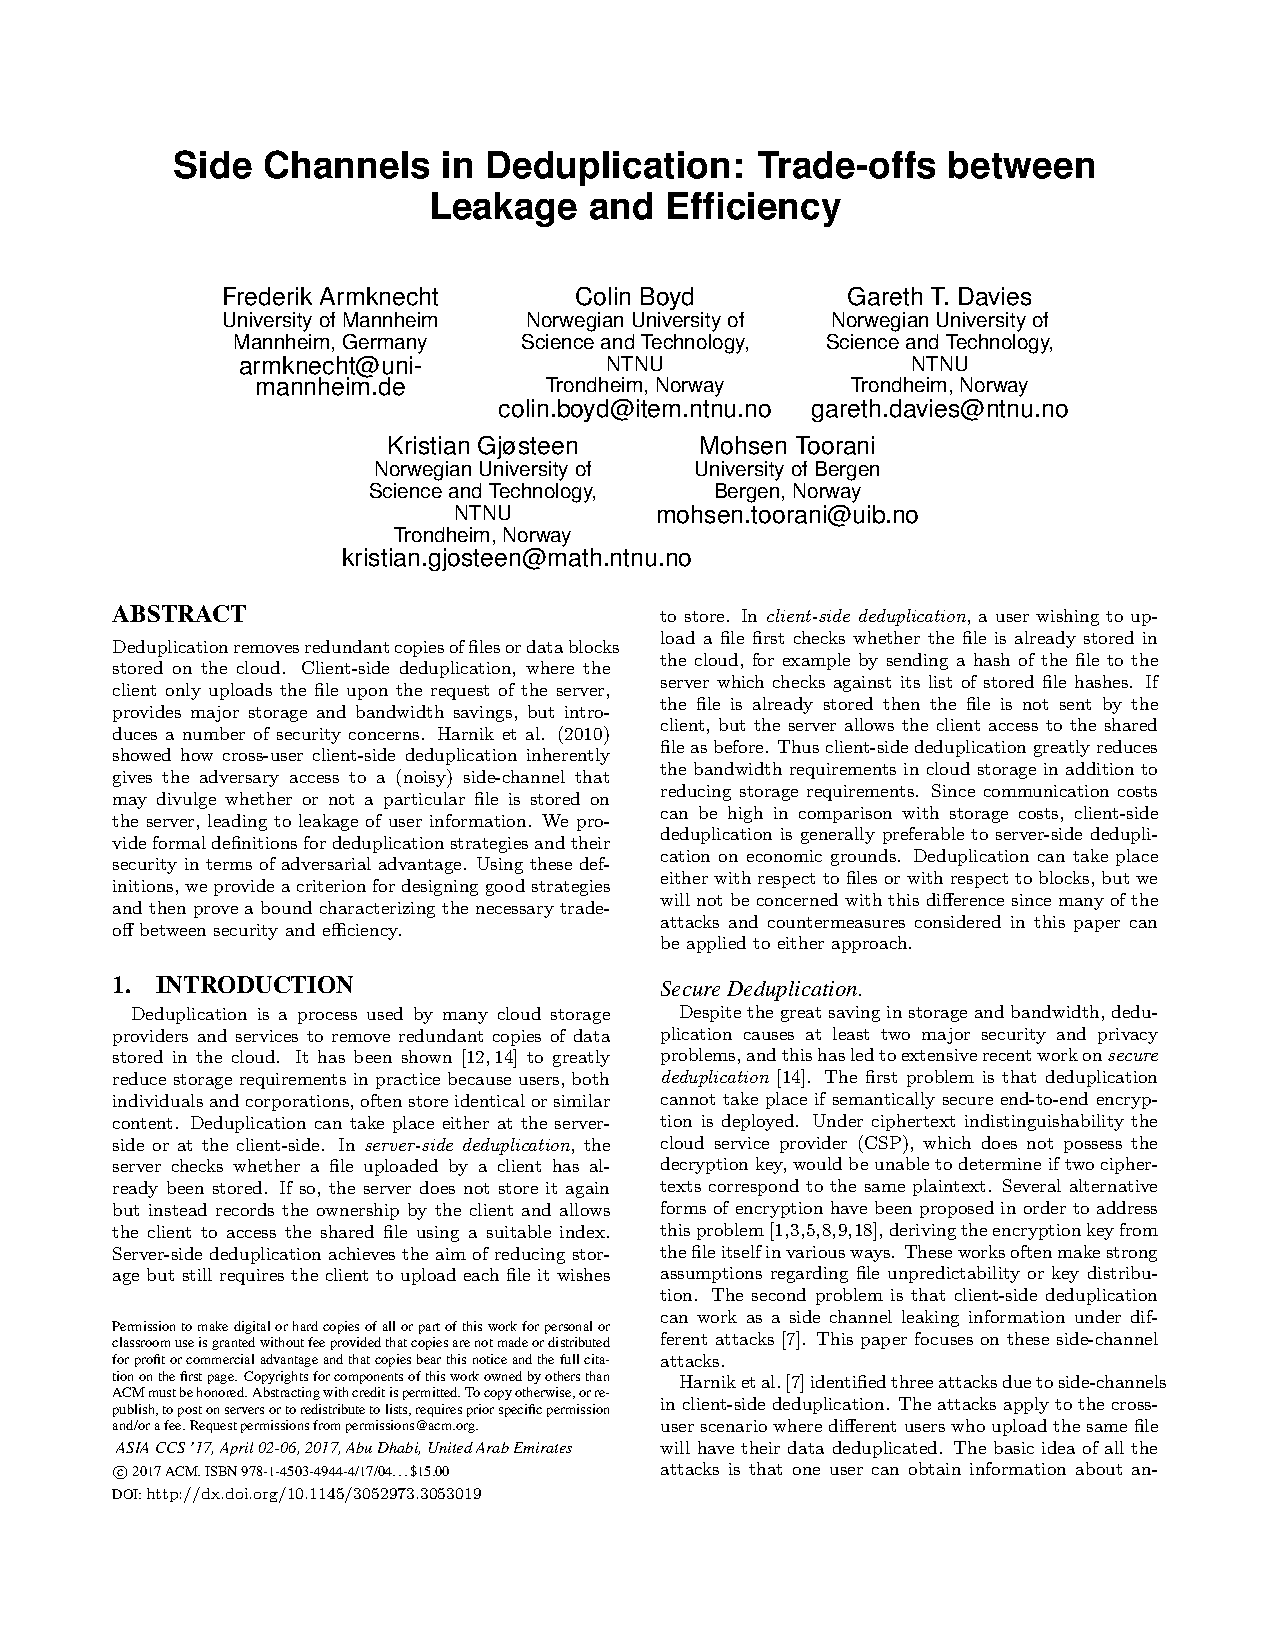
\includegraphics[width=14.5cm]{translate-1.pdf} 
    \label{fig:}
\end{figure}
\begin{figure}[!htb]
    \small
    \centering
    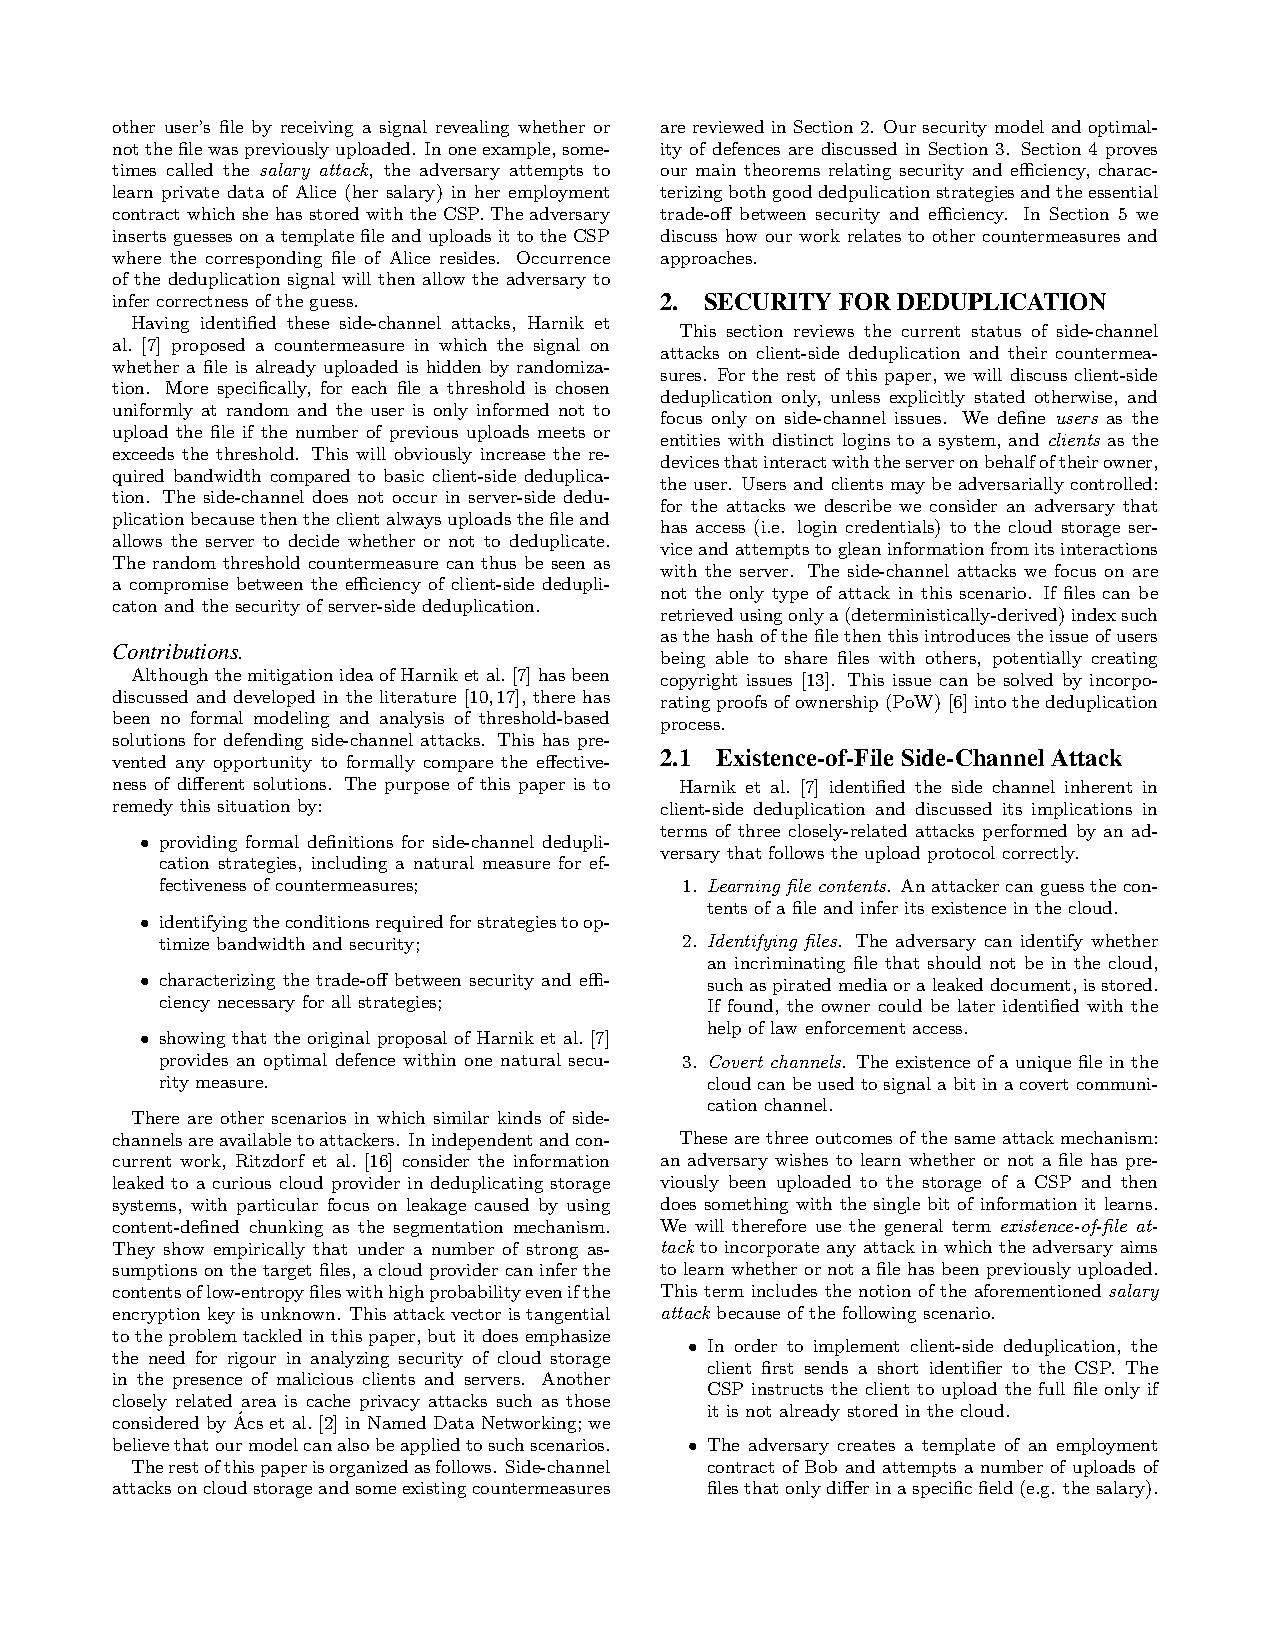
\includegraphics[width=\linewidth]{translate-2.pdf} 
    \label{fig:}
\end{figure}
%
%
\thesistranslationchinese
%
\section{引言}

重复数据删除是许多云存储提供商和服务使用的一个过程,用于删除存储在云中的冗余数据副本。因为个人和公司的用户通常存储相同或相似的内容,其在实践中大大降低了存储要求[12,14]。重复数据删除可以在服务器端或客户端进行。在服务器端重复数据删除中,服务器会检查客户端上载的文件是否已经存储。如果是这样,服务器不会再次存储它,而是由客户端记录文件所有权,并允许客当前户端使用合适的索引访问该共享文件。服务器端重复数据删除实现了减少存储空间占用的目的,但仍然要求客户端上载它希望存储的每个文件。在客户端重复数据删除中,希望首先上载文件的用户检查文件是否已经存储在云中,例如通过将文件的散列发送到服务器,该服务器检查其存储的文件散列列表。如果文件已经存储,则客户端不会发送文件,但服务器允许客户端像以前一样访问共享文件。因此,除了降低存储要求之外,客户端重复数据删除还可以大大降低云存储的带宽需求。由于与存储成本相比,通信成本可能更高。出于经济原因,客户端重复数据删除通常优于服务器端重复数据删除。重复数据删除可以针对文件或针对数据块进行,但我们不会关注这种差异,因为本文中考虑的许多攻击和对策都可以应用于其中任何一种方法。

\subsection{加密重复数据删除}

尽管重复数据删除中存储和带宽节省了很多,但其至少会导致两个主要的安全和隐私问题,这些问题在安全重复数据删除方面的有广泛的工作[14]。第一个问题是,如果部署了端到端加密方法,则无法进行重复数据删除。因为在密文不可区分的情况下,不具有解密密钥的云服务提供商(CSP)将无法确定两个密文是否对应于相同的明文。为了解决这个问题[1,3,5,8,9,18],已经提出了几种替代的加密形式,以各种方式从文件本身导出加密密钥。这些工作通常会对文件的不可预测性或关键分布做出强有力的假设。第二个问题是客户端重复数据删除可以作为在不同攻击下泄露信息的辅助渠道[7]。本文重点介绍这些侧通道攻击。

Harnik等人[7]提出了客户端重复数据删除中由于侧通道引起的三种攻击。这些攻击适用于跨用户的重复数据删除方案(其中上载相同文件的不同用户将对其数据进行重复数据删除)。这些攻击的基本思想是,一个用户可以通过接收显示文件是否已经上载的信号来获取有关另一个用户文件的信息。在一个例子中(有时称为工资攻击),对手试图在Alice与CSP存储的雇佣合同中学习她的私人数据(她的工资)。攻击者在模板文件上插入猜测的数据并将其上传到Alice的相应文件所在的CSP。然后,对手通过重复数据删除信号的出现与否推断出猜测的正确性。

确定了这些侧通道攻击后,Harnik等人[7]提出了一种对策,其中关于文件是否已经上传的信号被随机化隐藏。更具体地,对于每个文件,随机均匀地选择阈值,如果先前上载的次数满足或超过阈值,则通知用户不上载文件。与基本的客户端重复数据删除相比,这显然会增加系统所需的带宽。同时,在服务器端重复数据删除中不会出现侧信道攻击,因为客户端总是上传文件并由服务器决定是否进行重复数据删除。因此,随机阈值对策可视为客户端重复数据删除的效率与服务器端重复数据删除的安全性之间的折衷选择。

\subsection{主要贡献}

虽然Harnik等的基于阈值的解决方案来保护侧通道攻击的对策[7]已经在文献[10,17]中进行了讨论和开发,但没有进行正式的建模和分析。本文正式的比较不同解决方案的有效性:

\begin{itemize}
    \item 为侧信道重复数据删除策略提供正式定义,包括对策的有效性的自然衡量标准。
    \item 确定优化带宽和安全性所需的条件。
    \item 描述所有策略所需的安全性和效率之间如何进行权衡。
    \item 证明Harnik等人的原始提案[7]在一个自然安全措施中可以提供最佳防御效果。
\end{itemize}


在其他情况下,攻击者可以使用类似的侧信道。在独立而同时的工作中,Ritzdorf等人[16]考虑在重复数据删除存储系统中泄漏给好奇的云提供商的信息,并且特别关注使用内容定义的分块作为数据块分块机制引起的泄漏。他们凭经验证明,在对目标文件的许多强假设下,即使加密密钥未知,云提供商也可以高概率地推断出低熵文件的内容。这个攻击向量与本文讨论的问题相关,它强调了在存在恶意客户端和服务器的情况下分析云存储安全性的严格要求。另一个密切相关的领域是缓存隐私攻击,例如Acs等人[2]所考虑的那些在命名数据网络中的攻击。我们相信我们的模型也可以应用于这种情况。

本文的其余部分安排如下。第2节回顾了对云存储的侧通道攻击和一些现有的对策。第3节讨论了我们的安全模型和防御的最优性。第4节证明了我们关于安全性和效率的主要定理,同时描述了良好的策略如何在安全与效率之间做基本权衡。 在第5节中,我们将讨论我们的工作与其他对策和方法的相关性。



\end{document}
